% Analisi dei Requisiti
% da compilare con il comando pdflatex Analisi_dei_requisiti_x.x.x.tex

% Dichiarazioni di ambiente e inclusione di pacchetti
% da usare tramite il comando % Dichiarazioni di ambiente e inclusione di pacchetti
% da usare tramite il comando % Dichiarazioni di ambiente e inclusione di pacchetti
% da usare tramite il comando \input{../../util/hx-ambiente}

\documentclass[a4paper,titlepage]{article}
\usepackage[T1]{fontenc}
\usepackage[utf8]{inputenc}
\usepackage[english,italian]{babel}
\usepackage{microtype}
\usepackage{lmodern}
\usepackage{underscore}
\usepackage{graphicx}
\usepackage{eurosym}
\usepackage{float}
\usepackage{fancyhdr}
\usepackage[table]{xcolor}
\usepackage{longtable}
\usepackage{chngpage}
\usepackage{grffile}
\usepackage[titles]{tocloft}
\usepackage{hyperref}
\hypersetup{hidelinks}

\usepackage{../../util/hx-vers}
\usepackage{../../util/hx-macro}
\usepackage{../../util/hx-front}

% solo se si vuole una nuova pagina ad ogni \section:
\usepackage{titlesec}
\newcommand{\sectionbreak}{\clearpage}

% stile di pagina:
\pagestyle{fancy}

% solo se si vuole eliminare l'indentazione ad ogni paragrafo:
\setlength{\parindent}{0pt}

% intestazione:
\lhead{\Large{\proj}}
\rhead{
\includegraphics[keepaspectratio=true,width=50px]{../../util/hivex_logo2.png}}
\renewcommand{\headrulewidth}{0.4pt}

% pie' di pagina:
\lfoot{\email}
\rfoot{\thepage}
\cfoot{}
\renewcommand{\footrulewidth}{0.4pt}

% spazio verticale tra le celle di una tabella:
\renewcommand{\arraystretch}{1.5}

% profondità di indicizzazione:
\setcounter{tocdepth}{4}
\setcounter{secnumdepth}{4}


\documentclass[a4paper,titlepage]{article}
\usepackage[T1]{fontenc}
\usepackage[utf8]{inputenc}
\usepackage[english,italian]{babel}
\usepackage{microtype}
\usepackage{lmodern}
\usepackage{underscore}
\usepackage{graphicx}
\usepackage{eurosym}
\usepackage{float}
\usepackage{fancyhdr}
\usepackage[table]{xcolor}
\usepackage{longtable}
\usepackage{chngpage}
\usepackage{grffile}
\usepackage[titles]{tocloft}
\usepackage{hyperref}
\hypersetup{hidelinks}

\usepackage{../../util/hx-vers}
\usepackage{../../util/hx-macro}
\usepackage{../../util/hx-front}

% solo se si vuole una nuova pagina ad ogni \section:
\usepackage{titlesec}
\newcommand{\sectionbreak}{\clearpage}

% stile di pagina:
\pagestyle{fancy}

% solo se si vuole eliminare l'indentazione ad ogni paragrafo:
\setlength{\parindent}{0pt}

% intestazione:
\lhead{\Large{\proj}}
\rhead{
\includegraphics[keepaspectratio=true,width=50px]{../../util/hivex_logo2.png}}
\renewcommand{\headrulewidth}{0.4pt}

% pie' di pagina:
\lfoot{\email}
\rfoot{\thepage}
\cfoot{}
\renewcommand{\footrulewidth}{0.4pt}

% spazio verticale tra le celle di una tabella:
\renewcommand{\arraystretch}{1.5}

% profondità di indicizzazione:
\setcounter{tocdepth}{4}
\setcounter{secnumdepth}{4}


\documentclass[a4paper,titlepage]{article}
\usepackage[T1]{fontenc}
\usepackage[utf8]{inputenc}
\usepackage[english,italian]{babel}
\usepackage{microtype}
\usepackage{lmodern}
\usepackage{underscore}
\usepackage{graphicx}
\usepackage{eurosym}
\usepackage{float}
\usepackage{fancyhdr}
\usepackage[table]{xcolor}
\usepackage{longtable}
\usepackage{chngpage}
\usepackage{grffile}
\usepackage[titles]{tocloft}
\usepackage{hyperref}
\hypersetup{hidelinks}

\usepackage{../../util/hx-vers}
\usepackage{../../util/hx-macro}
\usepackage{../../util/hx-front}

% solo se si vuole una nuova pagina ad ogni \section:
\usepackage{titlesec}
\newcommand{\sectionbreak}{\clearpage}

% stile di pagina:
\pagestyle{fancy}

% solo se si vuole eliminare l'indentazione ad ogni paragrafo:
\setlength{\parindent}{0pt}

% intestazione:
\lhead{\Large{\proj}}
\rhead{
\includegraphics[keepaspectratio=true,width=50px]{../../util/hivex_logo2.png}}
\renewcommand{\headrulewidth}{0.4pt}

% pie' di pagina:
\lfoot{\email}
\rfoot{\thepage}
\cfoot{}
\renewcommand{\footrulewidth}{0.4pt}

% spazio verticale tra le celle di una tabella:
\renewcommand{\arraystretch}{1.5}

% profondità di indicizzazione:
\setcounter{tocdepth}{4}
\setcounter{secnumdepth}{4}


\version{2.0.0}
\creaz{19 dicembre 2016}
\author{\AZ}
\supervisor{\GG}
\uso{esterno}
\dest{\TV, \RC, \ZU}
\title{Analisi dei Requisiti}

\begin{document}
\maketitle
% diario delle modifiche per il piano di progetto
% da includere con % diario delle modifiche per il piano di progetto
% da includere con % diario delle modifiche per il piano di progetto
% da includere con \include{diario}

\begin{diario}
	1.0.1 & {\GG} (Responsabile) & 03/02/2017 & Correzione degli errori individuati nelle prime tre sezioni del documento \\ \hline
	1.0.0 & {\PB} (Responsabile) & 09/01/2017 & Approvazione documento \\ \hline
	0.1.0 & {\MM} (Verificatore) & 07/01/2017 & Verifica documento \\ \hline
	0.0.9 & {\PB} (Responsabile) & 05/01/2017 & Stesura Organigramma \\ \hline
	0.0.8 & {\LB} (Responsabile) & 05/01/2017 & Stesura Consuntivo di Periodo \\ \hline
	0.0.7 & {\LB} (Responsabile) & 04/01/2017 & Stesura Preventivo di Periodo \\ \hline
	0.0.6 & {\LB} (Responsabile) & 03/01/2017 & Inserimento Gantt Diagrammi delle Attività \\ \hline
	0.0.5 & {\PB} (Responsabile) & 29/12/2016 & Stesura Pianificazione delle Attività \\ \hline
	0.0.4 & {\PB} (Responsabile) & 28/12/2016 & Stesura Introduzione \\ \hline
	0.0.3 & {\LB} (Responsabile) & 27/12/2016 & Stesura Modello di sviluppo \\ \hline
	0.0.2 & {\PB} (Responsabile) & 27/12/2016 & Stesura Analisi dei Rischi \\ \hline
	0.0.1 & {\LB} (Responsabile) & 26/12/2016 & Stesura scheletro \\ \hline
\end{diario}

\begin{diario}
	1.0.1 & {\GG} (Responsabile) & 03/02/2017 & Correzione degli errori individuati nelle prime tre sezioni del documento \\ \hline
	1.0.0 & {\PB} (Responsabile) & 09/01/2017 & Approvazione documento \\ \hline
	0.1.0 & {\MM} (Verificatore) & 07/01/2017 & Verifica documento \\ \hline
	0.0.9 & {\PB} (Responsabile) & 05/01/2017 & Stesura Organigramma \\ \hline
	0.0.8 & {\LB} (Responsabile) & 05/01/2017 & Stesura Consuntivo di Periodo \\ \hline
	0.0.7 & {\LB} (Responsabile) & 04/01/2017 & Stesura Preventivo di Periodo \\ \hline
	0.0.6 & {\LB} (Responsabile) & 03/01/2017 & Inserimento Gantt Diagrammi delle Attività \\ \hline
	0.0.5 & {\PB} (Responsabile) & 29/12/2016 & Stesura Pianificazione delle Attività \\ \hline
	0.0.4 & {\PB} (Responsabile) & 28/12/2016 & Stesura Introduzione \\ \hline
	0.0.3 & {\LB} (Responsabile) & 27/12/2016 & Stesura Modello di sviluppo \\ \hline
	0.0.2 & {\PB} (Responsabile) & 27/12/2016 & Stesura Analisi dei Rischi \\ \hline
	0.0.1 & {\LB} (Responsabile) & 26/12/2016 & Stesura scheletro \\ \hline
\end{diario}

\begin{diario}
	1.0.1 & {\GG} (Responsabile) & 03/02/2017 & Correzione degli errori individuati nelle prime tre sezioni del documento \\ \hline
	1.0.0 & {\PB} (Responsabile) & 09/01/2017 & Approvazione documento \\ \hline
	0.1.0 & {\MM} (Verificatore) & 07/01/2017 & Verifica documento \\ \hline
	0.0.9 & {\PB} (Responsabile) & 05/01/2017 & Stesura Organigramma \\ \hline
	0.0.8 & {\LB} (Responsabile) & 05/01/2017 & Stesura Consuntivo di Periodo \\ \hline
	0.0.7 & {\LB} (Responsabile) & 04/01/2017 & Stesura Preventivo di Periodo \\ \hline
	0.0.6 & {\LB} (Responsabile) & 03/01/2017 & Inserimento Gantt Diagrammi delle Attività \\ \hline
	0.0.5 & {\PB} (Responsabile) & 29/12/2016 & Stesura Pianificazione delle Attività \\ \hline
	0.0.4 & {\PB} (Responsabile) & 28/12/2016 & Stesura Introduzione \\ \hline
	0.0.3 & {\LB} (Responsabile) & 27/12/2016 & Stesura Modello di sviluppo \\ \hline
	0.0.2 & {\PB} (Responsabile) & 27/12/2016 & Stesura Analisi dei Rischi \\ \hline
	0.0.1 & {\LB} (Responsabile) & 26/12/2016 & Stesura scheletro \\ \hline
\end{diario}
\tableofcontents
\listoffigures



\newcommand{\myimg}[1] {
	\begin{figure}[H]
		\makebox[\textwidth][c] {
			\includegraphics[width=1.1\textwidth]{Diagrammi casi d'uso/#1}
		}
		\caption{#1}
		\label{#1}
	\end{figure}
}

\newcommand{\myimgsmall}[1] {
	\begin{figure}[H]
		\makebox[\textwidth][c] {
			\includegraphics[width=0.9\textwidth]{Diagrammi casi d'uso/#1}
		}
		\caption{#1}
		\label{#1}
	\end{figure}
}

\newcommand{\myimgvsmall}[1] {
	\begin{figure}[H]
		\makebox[\textwidth][c] {
			\includegraphics[width=0.5\textwidth]{Diagrammi casi d'uso/#1}
		}
		\caption{#1}
		\label{#1}
	\end{figure}
}





%%%%%%%%%%%%%%%%
%%  Introduzione
%%%%%%%%%%%%%%%%

\section{Introduzione}

\subsection{Scopo del documento}
Questo documento ha lo scopo di elencare, classificare e tracciare i requisiti del prodotto \proj{} come identificati dal gruppo \hx{}.

L'individuazione di tali requisiti si è svolta dapprima tramite l'analisi del relativo capitolato d'appalto e successivamente attraverso una serie di incontri, sia interni al team che in presenza del committente.

Con il presente documento il gruppo \hx{} si impegna a sviluppare un prodotto che implementi le caratteristiche di seguito elencate.

\subsection{Scopo del prodotto}
\scopo

\subsection{Glossario}
\presgloss

\subsection{Riferimenti}
\subsubsection{Riferimenti normativi}
\begin{itemize}
	\item Norme di Progetto: \NdP;
	\item Capitolato d'appalto C6, \proj: \url{www.math.unipd.it/~tullio/IS-1/2016/Progetto/C6.pdf}, visitato in data 08/02/2017.
\end{itemize}

\subsubsection{Riferimenti informativi}
\begin{itemize}
	\item \textbf{Studio di Fattibilità}: \SdF;
	\item \textbf{Diagrammi dei casi d'uso}: \\
	\url{www.math.unipd.it/~tullio/IS-1/2016/Dispense/E01b.pdf}, visitato in data 08/02/2017;
	\item \textbf{Analisi dei requisiti}: \\
	\url{www.math.unipd.it/~tullio/IS-1/2016/Dispense/L06.pdf}, visitato in data 08/02/2017.
\end{itemize}





%%%%%%%%%%%%%%%%%%%%%%%%
%%  Descrizione generale
%%%%%%%%%%%%%%%%%%%%%%%%

\section{Descrizione generale}

\subsection{Obiettivo del prodotto}
Il prodotto sviluppato ha come scopo primario quello di fornire un editor in grado di supportare e guidare l'utente nella progettazione e nella codifica dell'applicativo desiderato e generare codice eseguibile, sulla base delle informazioni contenute nei diagrammi realizzati.

In particolare, il software risulterà orientato alla realizzazione di programmi appartenenti ad uno specifico dominio applicativo: quello dei giochi da tavolo.

\subsection{Funzioni del prodotto}
In dettaglio, all'interno di \proj{} sarà possibile:
\begin{itemize}
	\item definire un \gloss{diagramma delle classi};
	\item definire i diagrammi delle attività (con alcune modifiche rispetto al diagramma standard) dei metodi descritti nel diagramma delle classi;
	\item generare in modo automatico del codice che potrà, qualora l'utente abbia correttamente progettato la sua applicazione, essere compilato ed eseguito senza bisogno di apportare alcuna modifica a mano.
	\item salvare e caricare successivamente il proprio progetto sviluppato con \proj.
\end{itemize}

\subsection{Caratteristiche degli utenti}
Il prodotto \proj{} si rivolge principalmente ad una categoria di utenti ben specifica: quella dei programmatori o, in generale, dei lavoratori impiegati nell'ambito informatico con una buona conoscenza della programmazione.

In particolare, è richiesto che l'utente dell'editor abbia un certo grado di familiarità con i seguenti concetti:
\begin{itemize}
	\item Le principali convenzioni della modellazione UML e, nello specifico, i diagrammi delle classi e i diagrammi delle attività.
	\item Le astrazioni e i paradigmi della programmazione orientata agli oggetti; infatti il linguaggio target generato, i diagrammi e le funzionalità offerte suggeriscono che l'architettura dell'applicativo da realizzarsi sia ben strutturata in moduli funzionali specifici e distinti.
\end{itemize}
Per garantire inoltre una comprensione accurata e completa dell'insieme di funzionalità implementate, il prodotto sarà corredato di un manuale utente completo delle indicazioni necessarie per poterne fruire in modo efficace.

\subsection{Piattaforma di esecuzione}
Il prodotto sviluppato risulterà fruibile da qualsiasi piattaforma desktop con operante un browser web compatibile con le tecnologie HTML5, CSS3 e JavaScript. In particolare, l'elenco dei browser il cui supporto è garantito è contenuto nella sezione \ref{sec:reqvincolo} relativa ai requisiti di vincolo.

\subsection{Vincoli generali}
Si tiene conto dei seguenti vincoli:
\begin{itemize}
	\item I file prodotti dal programma sono modificabili esclusivamente dal programma stesso. Eventuali modifiche di esso sono possibili ma non garantiscono la compatibilità con l'applicativo, che potrà rifiutare il progetto modificato.
	\item La correttezza di eventuali spezzoni di codice inseriti a mano dall'utente nel linguaggio target sono completa responsabilità di quest'ultimo.
\end{itemize}





%%%%%%%%%%%%%%
%%  Casi d'uso
%%%%%%%%%%%%%%

\section{Casi d'uso}
All'interno di questa sezione vengono elencati i casi d'uso rilevanti per il prodotto \proj{} individuati e definiti attraverso l'analisi del capitolato d'appalto, gli incontri con il proponente e le riunioni interne al team \hx{}.

La struttura e le convenzioni usate in ogni \gloss{caso d'uso} sono specificate all'interno del documento \NdP.

Si noti che, per esigenze tipografiche, è possibile che certe figure siano state posizionate immediatamente dopo l'intera esposizione del caso d'uso. Esse sono comunque rintracciabili tramite il loro identificatore univoco.

\subsection{UC1: Pagina Iniziale}
\label{UC1}
\myimg{UC1 - Pagina Iniziale}
\begin{itemize}
	\item \textbf{Attori}: Utente;
	\item \textbf{Descrizione}: nella pagina iniziale l'attore crea un nuovo progetto oppure ne apre uno già esistente; successivamente l'attore può:
	\begin{itemize}
		\item realizzare e gestire un diagramma delle classi;
		\item realizzare e gestire un \gloss{diagramma delle attività} per ogni metodo presente nel diagramma delle classi;
		\item salvare le modifiche apportate al progetto (se questo è stato caricato);
		\item generare l'applicativo realizzato.
	\end{itemize}
	\item \textbf{Precondizione}: il sistema risulta avviato e mostra la pagina iniziale dell'applicazione;
	\item \textbf{Postcondizione}: il sistema ha ricevuto tutti gli input dall'attore sulle operazioni che vuole effettuare;
	\item \textbf{\gloss{Scenario} principale}:
	\begin{enumerate}
		\item l'attore può aprire un progetto esistente (UC2);
		\item l'attore può creare un nuovo progetto (UC3);
		\item l'attore può realizzare e gestire un diagramma delle classi (UC4);
		\item l'attore può realizzare e gestire un diagramma delle attività per ogni metodo presente nel diagramma delle classi (UC5);
		\item l'attore può salvare il progetto (UC6);
		\item l'attore può generare l'applicativo realizzato (UC7).
	\end{enumerate}
\end{itemize}

\subsection{UC2: Apertura Progetto}
\label{UC2}
\begin{itemize}
	\item \textbf{Attori}: Utente;
	\item \textbf{Descrizione}: l'attore può caricare un progetto precedentemente realizzato con il programma ora in uso allo scopo di apportarvi ulteriori modifiche e/o ampliamenti;
	\item \textbf{Precondizione}: il sistema avviato mostra la pagina iniziale dell'applicazione;
	\item \textbf{Postcondizione}: il sistema ha caricato il progetto selezionato, mostrandone il contenuto (come salvato dopo l'ultimo utilizzo);
	\item \textbf{Scenario principale}: l'attore carica il progetto selezionato;
	\item \textbf{Estensioni}: l'attore visualizza un messaggio d'errore riguardo al file inserito (UC2.1).
\end{itemize}

\subsubsection{UC2.1: Messaggio d'errore caricamento file}
\label{UC2.1}
\begin{itemize}
	\item \textbf{Attori}: Utente;
	\item \textbf{Descrizione}: l'attore visualizza un opportuno messaggio d'errore nel caso in cui tenti di inserire un file incompatibile rispetto all'editor in uso;
	\item \textbf{Precondizione}: l'attore ha selezionato per il caricamento un file con estensione incompatibile;
	\item \textbf{Postcondizione}: il sistema visualizza un messaggio d'errore per informare l'utente;
	\item \textbf{Scenario principale}: l'attore visualizza un messaggio d'errore che indica l'incompatibilità del file richiesto per il caricamento.
\end{itemize}

\subsection{UC3: Nuovo Progetto}
\label{UC3}
\begin{itemize}
	\item \textbf{Attori}: Utente;
	\item \textbf{Descrizione}: l'attore può creare un nuovo progetto;
	\item \textbf{Precondizione}: il sistema avviato mostra la pagina iniziale dell'applicazione;
	\item \textbf{Postcondizione}: il sistema crea un progetto vuoto e presenta all'attore un diagramma delle classi vuoto con un menù;
	\item \textbf{Scenario principale}:
	\begin{itemize} % >>> disegno con Astah? UC3.1 <<<
		\item l'attore deve inserire il nome del progetto.
	\end{itemize}
\end{itemize}

\subsubsection{UC3.1: Inserimento Nome Progetto}
\label{UC3.1}
\begin{itemize}
	\item \textbf{Attori}: Utente;
	\item \textbf{Descrizione}: l'attore deve inserire un nome da assegnare al nuovo progetto da creare;
	\item \textbf{Precondizione}: il sistema avviato mostra il form per l'inserimento dei dati;
	\item \textbf{Postcondizione}: il sistema crea un progetto vuoto;
	\item \textbf{Scenario principale}: l'attore inserisce il nome del nuovo progetto.
\end{itemize}

\subsection{UC4: Realizzazione Diagramma delle Classi}
\label{UC4}
\myimgsmall{UC4 - Realizzazione Diagramma delle Classi}
\begin{itemize}
	\item \textbf{Attori}: Utente;
	\item \textbf{Descrizione}: l'attore realizza e gestisce un diagramma delle classi con la possibilità di aggiungere nuovi elementi e rimuovere elementi precedentemente inseriti che non corrispondono più alle sue intenzioni di progettazione;
	\item \textbf{Precondizione}: il sistema è avviato e mostra il contenuto di un progetto;
	\item \textbf{Postcondizione}: il sistema visualizza il diagramma delle classi risultante dalla gestione operata dall'utente;
	\item \textbf{Scenario principale}:
	\begin{enumerate}
		\item l'attore può inserire un BloccoClasse (UC4.1);
		\item l'attore può inserire una classe (UC4.2);
		\item l'attore può inserire un'interfaccia (UC4.3);
		\item l'attore può inserire un BloccoRelazione (UC4.4);
		\item l'attore può inserire un'associazione (UC4.5);
		\item l'attore può inserire una generalizzazione (UC4.6);
		\item l'attore può inserire un'implementazione (UC4.7);
		\item l'attore può inserire un commento (UC4.8);
		\item l'attore può rimuovere un BloccoClasse (UC4.9);
		\item l'attore può rimuovere un BloccoRelazione (UC4.10);
		\item l'attore può rimuovere un commento (UC4.11);
		\item l'attore può modificare un BloccoClasse (UC4.12);
		\item l'attore può modificare una classe (UC4.13);
		\item l'attore può modificare un BloccoRelazione (UC4.14);
		\item l'attore può modificare un'associazione (UC4.15);
		\item l'attore può modificare un commento (UC4.16).
	\end{enumerate}
\end{itemize}

\subsubsection{UC4.1: Inserimento BloccoClasse}
\label{UC4.1}
\begin{itemize}
	\item \textbf{Attori}: Utente;
	\item \textbf{Descrizione}: l'attore inserisce i dati di una classe;
	\item \textbf{Precondizione}: il sistema è avviato, mostra il contenuto di un particolare progetto ed è nell'area per la realizzazione e gestione del diagramma delle classi. Viene visualizzata la classe;
	\item \textbf{Postcondizione}: il sistema ha ricevuto tutti i dati dall'attore sulla classe e mostra il diagramma delle classi;
	\item \textbf{Scenario principale}:
	\begin{enumerate}
		\item l'attore deve inserire il nome della classe/interfaccia (univoco) (UC4.1.1);
		%%\item l'attore visualizza un messaggio d'errore per l'inserimento del nome della classe/interfaccia (UC4.1.2);
		\item l'attore può aggiungere un metodo (UC4.1.2);
		\item l'attore può rimuovere un metodo (UC4.1.3);
		\item l'attore può espandere la lista dei metodi (UC4.1.4);
		\item l'attore può ridurre la lista deii metodi (UC4.1.5).
	\end{enumerate}
\end{itemize}

\paragraph{UC4.1.1: Inserimento Nome Classe/Interfaccia}
\label{UC4.1.1}
\begin{itemize}
	\item \textbf{Attori}: Utente;
	\item \textbf{Descrizione}: l'attore inserisce il nome (univoco) per la classe/interfaccia corrente;
	\item \textbf{Precondizione}: il sistema è avviato, mostra il contenuto di un particolare progetto ed è nell'area per la realizzazione e gestione del diagramma delle classi. Viene visualizzata la classe selezionata;
	\item \textbf{Postcondizione}: il sistema ha ricevuto il dato richiesto e lo visualizza nel diagramma delle classi;
	\item \textbf{Scenario principale}: l'attore inserisce il nome della classe/interfaccia;
	%%\item \textbf{Estensioni}: l'attore visualizza un messaggio d'errore riguardo al dato inserito (UC4.1.2).
\end{itemize}

%\subparagraph{UC4.1.2: Visualizzazione Errore Inserimento Nome Classe/Interfaccia}
%\label{UC4.1.2}
%\begin{itemize}
%	\item \textbf{Attori}: Utente;
%	\item \textbf{Descrizione}: l'attore può visualizzare un messaggio d'errore nel caso si fossero verificati uno o più scenari alternativi %durante la fase di inserimento del nome;
%	\item \textbf{Precondizione}: il sistema ha ricevuto informazion errate o insufficienti per l'inserimento del nome;
%	\item \textbf{Postcondizione}: il sistema avvisa l'attore dell'errore verificatosi, tramite un opportuno messaggio;
%	\item \textbf{Scenario principale}: l'attore visualizza un messaggio d'errore.
%\end{itemize}


%%%%%%%%%%%%%%%%%%%%%%%%%%%%%%%%
\paragraph{UC4.1.2: Inserimento Metodo BloccoClasse}
\label{UC4.1.2}
%%\myimg{UC4.1.2 - Inserimento Metodo}
\begin{itemize}
	\item \textbf{Attori}: Utente;
	\item \textbf{Descrizione}: l'attore inserisce un metodo per la classe;
	\item \textbf{Precondizione}:  il sistema è avviato, mostra il contenuto di un particolare progetto ed è nell'area per la realizzazione e gestione del diagramma delle classi. Viene visualizzata la classe;
	\item \textbf{Postcondizione}: il sistema visualizza il metodo fornito dall'attore nella classe correntemente gestita dallo stesso;
	\item \textbf{Scenario principale}:
	\begin{enumerate}
		\item l'attore può scegliere la visibilità del metodo (UC4.1.2.1);
		\item l'attore deve inserire il nome del metodo (UC4.1.2.2);
		%\item l'attore visualizza un messaggio d'errore per l'inserimento del nome del metodo (UC4.1.3.3);
		\item l'attore può inserire un parametro del metodo (UC4.1.2.3);
		\item l'attore deve inserire il tipo di ritorno del metodo (UC4.1.2.4);
		\item l'attore può rimuovere un parametro del metodo (UC4.1.2.5).
	\end{enumerate}
	\item \textbf{Generalizzazioni}: Inserimento Metodo Classe (UC4.2.5).%%%%%%%%%%%%
\end{itemize}

\subparagraph{UC4.1.2.1: Inserimento Visibilità Metodo}
\label{UC4.1.2.1}
\begin{itemize}
	\item \textbf{Attori}: Utente;
	\item \textbf{Descrizione}: l'attore può scegliere la visibilità per il metodo;
	\item \textbf{Precondizione}:  il sistema è avviato, mostra il contenuto di un particolare progetto ed è nell'area per la realizzazione e gestione del diagramma delle classi. Viene visualizzata la classe;
	\item \textbf{Postcondizione}: il sistema ha ricevuto il dato richiesto e lo visualizza nel diagrama delle classi;
	\item \textbf{Scenario principale}: l'attore sceglie la visibilità del metodo altrimenti viene applicato il valore di default.
\end{itemize}

\subparagraph{UC4.1.2.2: Inserimento Nome Metodo}
\label{UC4.1.2.2}
\begin{itemize}
	\item \textbf{Attori}: Utente;
	\item \textbf{Descrizione}: l'attore deve inserire il nome del metodo, che deve essere univoco nella classe correntemente gestita rispetto ad altri metodi già inseriti con la stessa segnatura;
	\item \textbf{Precondizione}: il sistema è avviato, mostra il contenuto di un particolare progetto ed è nell'area per la realizzazione e gestione del diagramma delle classi. Viene visualizzata la classe;
	\item \textbf{Postcondizione}: il sistema ha ricevuto il dato richiesto e lo visualizza nel diagrama delle classi;
	\item \textbf{Scenario principale}: l'attore inserisce il nome del metodo;
	%\item \textbf{Estensioni}: l'attore visualizza un messaggio d'errore riguardo al dato inserito (UC4.1.3.3).
\end{itemize}

%\subparagraph{UC4.1.3.3: Visualizzazione Errore Inserimento Nome Metodo}
%\label{UC4.1.3.3}
%\begin{itemize}
%	\item \textbf{Attori}: Utente;
%	\item \textbf{Descrizione}: l'attore può visualizzare un messaggio d'errore nel caso si fossero verificati uno o più scenari alternativi durante la fase di inserimento del nome;
%	\item \textbf{Precondizione}: il sistema ha ricevuto informazion errate o insufficienti per l'inserimento del nome;
%	\item \textbf{Postcondizione}: il sistema avvisa l'attore dell'errore verificatosi, tramite un opportuno messaggio;
%	\item \textbf{Scenario principale}: l'attore visualizza un messaggio d'errore.
%\end{itemize}

\subparagraph{UC4.1.2.3: Inserimento Parametro Metodo}
\label{UC4.1.2.3}
%\myimg{UC4.1.2.3 - Inserimento Parametro Metodo}
\begin{itemize}
	\item \textbf{Attori}: Utente;
	\item \textbf{Descrizione}: l'attore inserisce un parametro per il metodo corrente;
	\item \textbf{Precondizione}:  il sistema è avviato, mostra il contenuto di un particolare progetto ed è nell'area per la realizzazione e gestione del diagramma delle classi. Viene visualizzata la classe;
	\item \textbf{Postcondizione}: il sistema visualizza il parametro fornito dall'attore nella classe correntemente gestita dallo stesso;
	\item \textbf{Scenario principale}:
	\begin{enumerate}
		\item l'attore deve inserire il nome del parametro (UC4.1.2.3.1);
		\item l'attore deve inserire il tipo del parametro (UC4.1.2.3.2);
		\item l'attore può inserire il valore di default del parametro (UC4.1.2.3.3).
	\end{enumerate}
\end{itemize}

\subsubparagraph{UC4.1.2.3.1: Inserimento Nome Parametro}
\label{UC4.1.2.3.1}
\begin{itemize}
	\item \textbf{Attori}: Utente;
	\item \textbf{Descrizione}: l'attore deve inserire il nome del parametro del metodo, che deve essere univoco nel metodo correntemente gestito rispetto ad altri parametri già inseriti con lo stesso nome;
	\item \textbf{Precondizione}: il sistema è avviato, mostra il contenuto di un particolare progetto ed è nell'area per la realizzazione e gestione del diagramma delle classi. Viene visualizzata la classe;
	\item \textbf{Postcondizione}: il sistema ha ricevuto il dato richiesto e lo visualizza nel diagrama delle classi;
	\item \textbf{Scenario principale}: l'attore inserisce il nome del parametro.
\end{itemize}

\subsubparagraph{UC4.1.2.3.2: Inserimento Tipo Parametro}
\label{UC4.1.2.3.2}
\begin{itemize}
	\item \textbf{Attori}: Utente;
	\item \textbf{Descrizione}: l'attore deve inserire il tipo del parametro;
	\item \textbf{Precondizione}: il sistema è avviato, mostra il contenuto di un particolare progetto ed è nell'area per la realizzazione e gestione del diagramma delle classi. Viene visualizzata la classe;
	\item \textbf{Postcondizione}: il sistema ha ricevuto il dato richiesto e lo visualizza nel diagrama delle classi;
	\item \textbf{Scenario principale}: l'attore inserisce il tipo del parametro.
\end{itemize}

\subparagraph{UC4.1.2.3.3: Inserimento Valore Default Parametro}
\label{UC4.1.2.3.3}
\begin{itemize}
	\item \textbf{Attori}: Utente;
	\item \textbf{Descrizione}: l'attore può inserire il valore di default del parametro;
	\item \textbf{Precondizione}: il sistema è avviato, mostra il contenuto di un particolare progetto ed è nell'area per la realizzazione e gestione del diagramma delle classi. Viene visualizzata la classe;
	\item \textbf{Postcondizione}: il sistema ha ricevuto il dato richiesto e lo visualizza nel diagrama delle classi;
	\item \textbf{Scenario principale}: l'attore inserisce  il valore di default del parametro.
\end{itemize}

\subparagraph{UC4.1.2.4: Inserimento Tipo Ritorno Metodo}
\label{UC4.1.2.4}
\begin{itemize}
	\item \textbf{Attori}: Utente;
	\item \textbf{Descrizione}: l'attore deve inserire il tipo di ritorno del metodo;
	\item \textbf{Precondizione}: il sistema è avviato, mostra il contenuto di un particolare progetto ed è nell'area per la realizzazione e gestione del diagramma delle classi. Viene visualizzata la classe;
	\item \textbf{Postcondizione}: il sistema ha ricevuto il dato richiesto e lo visualizza nel diagrama delle classi;
	\item \textbf{Scenario principale}: l'attore inserisce il tipo di ritorno del metodo.
\end{itemize}

\subparagraph{UC4.1.2.5: Rimozione Parametro Metodo}
\label{UC4.1.2.5}
\begin{itemize}
	\item \textbf{Attori}: Utente;
	\item \textbf{Descrizione}: l'attore rimuove un parametro del metodo;
	\item \textbf{Precondizione}: il sistema è avviato, mostra il contenuto di un particolare progetto ed è nell'area per la realizzazione e gestione del diagramma delle classi. Viene visualizzata la classe;
	\item \textbf{Postcondizione}: il sistema rimuove il parametro selezionato per la rimozione;
	\item \textbf{Scenario principale}: l'attore rimuove il parametro selezionato.
\end{itemize}

\paragraph{UC4.1.3: Rimozione Metodo BloccoClasse}
\label{UC4.1.3}
\begin{itemize}
	\item \textbf{Attori}: Utente;
	\item \textbf{Descrizione}: l'attore può rimuovere un metodo precedentemente inserito;
	\item \textbf{Precondizione}: il sistema è avviato, mostra il contenuto di un particolare progetto ed è nell'area per la realizzazione e gestione del diagramma delle classi. Viene visualizzata la classe;
	\item \textbf{Postcondizione}: il sistema rimuove il metodo selezionato;
	\item \textbf{Scenario principale}: l'attore rimuove il metodo selezionato.
\end{itemize}

\paragraph{UC4.1.4: Riduzione Lista Metodi BloccoClasse}
\label{UC4.1.4}
\begin{itemize}
	\item \textbf{Attori}: Utente;
	\item \textbf{Descrizione}: l'attore può ridurre la lista dei metodi;
	\item \textbf{Precondizione}: il sistema è avviato, mostra il contenuto di un particolare progetto ed è nell'area per la realizzazione e gestione del diagramma delle classi. Viene visualizzata la classe;
	\item \textbf{Postcondizione}: il sistema visualizza la lista dei metodi della classe selezionata dall'utente in formato ridotto;
	\item \textbf{Scenario principale}: l'attore riduce la lista dei metodi della classe.
\end{itemize}

\paragraph{UC4.1.5: Espansione Lista Metodi BloccoClasse}
\label{UC4.1.5}
\begin{itemize}
	\item \textbf{Attori}: Utente;
	\item \textbf{Descrizione}: l'attore può espandere la lista dei metodi;
	\item \textbf{Precondizione}: il sistema è avviato, mostra il contenuto di un particolare progetto ed è nell'area per la realizzazione e gestione del diagramma delle classi. Viene visualizzata la classe;
	\item \textbf{Postcondizione}: il sistema visualizza la lista dei metodi della classe selezionata dall'utente in formato esteso;
	\item \textbf{Scenario principale}: l'attore estende la lista dei metodi della classe.
\end{itemize}

\subsubsection{UC4.2: Inserimento Classe}
\label{UC4.2}
\begin{itemize}
	\item \textbf{Attori}: Utente;
	\item \textbf{Descrizione}: l'attore inserisce i dati di una classe;
	\item \textbf{Precondizione}: il sistema è avviato, mostra il contenuto di un particolare progetto ed è nell'area per la realizzazione e gestione del diagramma delle classi. Viene visualizzata la classe;
	\item \textbf{Postcondizione}: il sistema ha ricevuto tutti i dati dall'attore sulla classe e mostra il diagramma delle classi;
	\item \textbf{Scenario principale}:
	\begin{enumerate}
		\item l'attore può aggiungere un attributo (UC4.2.1);
		\item l'attore può rimuovere un attributo (UC4.2.2);
		\item l'attore può espandere la lista degli attributi (UC4.2.3);
		\item l'attore può ridurre la lista degli attributi (UC4.2.4);
		\item l'attore può inserire dati aggiuntivi ad un metodo (UC4.2.5);
		\item l'attore può scegliere uno stereotipo tra quelli proposti (UC4.2.6);%%switch al diagramma delle attività: come lo inserisco????
		\item l'attore può specificare se la classe è astratta (UC4.2.7);
		\item l'attore può specificare se la classe è statica (UC4.2.8).
	\end{enumerate}
\end{itemize}

\paragraph{UC4.2.1: Inserimento Attributo Classe}
\label{UC4.2.1}
\begin{itemize}
	\item \textbf{Attori}: Utente;
	\item \textbf{Descrizione}: l'attore inserisce un attributo per la classe corrente;
	\item \textbf{Precondizione}:  il sistema è avviato, mostra il contenuto di un particolare progetto ed è nell'area per la realizzazione e gestione del diagramma delle classi. Viene visualizzata la classe;
	\item \textbf{Postcondizione}: il sistema visualizza l'attributo fornito dall'attore nella classe correntemente gestita dallo stesso;
	\item \textbf{Scenario principale}:
	\begin{enumerate}
		\item l'attore deve inserire il nome dell'attributo (UC4.2.1.1);
		\item l'attore deve inserire il tipo dell'attributo (UC4.2.1.2);
		\item l'attore può inserire la visibilità dell'attributo (UC4.2.1.3);
		\item l'attore può inserire il valore di default del parametro (UC4.2.1.4).
	\end{enumerate}
\end{itemize}

\subparagraph{UC4.2.1.1: Inserimento Nome Attributo}
\label{UC4.2.1.1}
\begin{itemize}
	\item \textbf{Attori}: Utente;
	\item \textbf{Descrizione}: l'attore deve inserire il nome dell'attributo del metodo;
	\item \textbf{Precondizione}: il sistema è avviato, mostra il contenuto di un particolare progetto ed è nell'area per la realizzazione e gestione del diagramma delle classi. Viene visualizzata la classe;
	\item \textbf{Postcondizione}: il sistema ha ricevuto il dato richiesto e lo visualizza nel diagrama delle classi;
	\item \textbf{Scenario principale}: l'attore inserisce il nome dell'attributo.
\end{itemize}

\subparagraph{UC4.2.1.2: Inserimento Tipo Attributo}
\label{UC4.2.1.2}
\begin{itemize}
	\item \textbf{Attori}: Utente;
	\item \textbf{Descrizione}: l'attore deve inserire il tipo dell'attributo;
	\item \textbf{Precondizione}: il sistema è avviato, mostra il contenuto di un particolare progetto ed è nell'area per la realizzazione e gestione del diagramma delle classi. Viene visualizzata la classe;
	\item \textbf{Postcondizione}: il sistema ha ricevuto il dato richiesto e lo visualizza nel diagrama delle classi;
	\item \textbf{Scenario principale}: l'attore inserisce il tipo dell'attributo.
\end{itemize}

\subparagraph{UC4.2.1.3: Inserimento Visibilità Attributo}
\label{UC4.2.1.3}
\begin{itemize}
	\item \textbf{Attori}: Utente;
	\item \textbf{Descrizione}: l'attore può inserire la visibilità dell'attributo;
	\item \textbf{Precondizione}: il sistema è avviato, mostra il contenuto di un particolare progetto ed è nell'area per la realizzazione e gestione del diagramma delle classi. Viene visualizzata la classe;
	\item \textbf{Postcondizione}: il sistema ha ricevuto il dato richiesto e lo visualizza nel diagrama delle classi;
	\item \textbf{Scenario principale}: l'attore inserisce la visibilità dell'attributo.
\end{itemize}

\subparagraph{UC4.2.1.4: Inserimento Valore Default Attributo}
\label{UC4.2.1.4}
\begin{itemize}
	\item \textbf{Attori}: Utente;
	\item \textbf{Descrizione}: l'attore può inserire il valore di default dell'attributo;
	\item \textbf{Precondizione}: il sistema è avviato, mostra il contenuto di un particolare progetto ed è nell'area per la realizzazione e gestione del diagramma delle classi. Viene visualizzata la classe;
	\item \textbf{Postcondizione}: il sistema ha ricevuto il dato richiesto e lo visualizza nel diagrama delle classi;
	\item \textbf{Scenario principale}: l'attore inserisce  il valore di default dell'attributo.
\end{itemize}

\paragraph{UC4.2.2: Rimozione Attributo Classe}
\label{UC4.2.2}
\begin{itemize}
	\item \textbf{Attori}: Utente;
	\item \textbf{Descrizione}: l'attore rimuove un attributo della classe;
	\item \textbf{Precondizione}: il sistema è avviato, mostra il contenuto di un particolare progetto ed è nell'area per la realizzazione e gestione del diagramma delle classi. Viene visualizzata la classe;
	\item \textbf{Postcondizione}: il sistema rimuove l'attributo selezionato per la rimozione;
	\item \textbf{Scenario principale}: l'attore rimuove l'attributo selezionato.
\end{itemize}

\paragraph{UC4.2.3: Riduzione Lista Attributi Classe}
\label{UC4.2.3}
\begin{itemize}
	\item \textbf{Attori}: Utente;
	\item \textbf{Descrizione}: l'attore può ridurre la lista degli attributi;
	\item \textbf{Precondizione}: il sistema è avviato, mostra il contenuto di un particolare progetto ed è nell'area per la realizzazione e gestione del diagramma delle classi. Viene visualizzata la classe;
	\item \textbf{Postcondizione}: il sistema visualizza la lista degli attributi della classe selezionata dall'utente in formato ridotto;
	\item \textbf{Scenario principale}: l'attore riduce la lista degli attributi della classe.
\end{itemize}

\paragraph{UC4.2.4: Espansione Lista Attributi Classe}
\label{UC4.2.4}
\begin{itemize}
	\item \textbf{Attori}: Utente;
	\item \textbf{Descrizione}: l'attore può espandere la lista degli attributi;
	\item \textbf{Precondizione}: il sistema è avviato, mostra il contenuto di un particolare progetto ed è nell'area per la realizzazione e gestione del diagramma delle classi. Viene visualizzata la classe;
	\item \textbf{Postcondizione}: il sistema visualizza la lista degli attrubuti della classe selezionata dall'utente in formato esteso;
	\item \textbf{Scenario principale}: l'attore estende la lista degli attributi della classe.
\end{itemize}

\paragraph{UC4.2.5: Inserimento Dati Aggiuntivi Metodo}
\label{UC4.2.5}
\begin{itemize}
	\item \textbf{Attori}: Utente;
	\item \textbf{Descrizione}: l'attore inserisce dei dati aggiuntivi ad un metodo per la classe corrente;
	\item \textbf{Precondizione}:  il sistema è avviato, mostra il contenuto di un particolare progetto ed è nell'area per la realizzazione e gestione del diagramma delle classi. Viene visualizzata la classe;
	\item \textbf{Postcondizione}: il sistema visualizza i dati forniti dall'attore nella classe correntemente gestita dallo stesso;
	\item \textbf{Scenario principale}:
	\begin{enumerate}
		\item l'attore può specificare se il metodo è astratto (UC4.2.5.1);
		\item l'attore può specificare se il metodo è statico (UC4.2.5.2).
	\end{enumerate}
\end{itemize}

\subparagraph{UC4.2.5.1: Specifica Metodo Astratto}
\label{UC4.2.5.1}
\begin{itemize}
	\item \textbf{Attori}: Utente;
	\item \textbf{Descrizione}: l'attore specificare se il metodo è astratto;
	\item \textbf{Precondizione}: il sistema è avviato, mostra il contenuto di un particolare progetto ed è nell'area per la realizzazione e gestione del diagramma delle classi. Viene visualizzata la classe;
	\item \textbf{Postcondizione}: il sistema ha ricevuto il dato richiesto e lo visualizza nel diagrama delle classi;
	\item \textbf{Scenario principale}: l'attore specifica che il metodo è astratto.
\end{itemize}

\subparagraph{UC4.2.5.2: Specifica Metodo Statico}
\label{UC4.2.5.2}
\begin{itemize}
	\item \textbf{Attori}: Utente;
	\item \textbf{Descrizione}: l'attore specificare se il metodo è statico;
	\item \textbf{Precondizione}: il sistema è avviato, mostra il contenuto di un particolare progetto ed è nell'area per la realizzazione e gestione del diagramma delle classi. Viene visualizzata la classe;
	\item \textbf{Postcondizione}: il sistema ha ricevuto il dato richiesto e lo visualizza nel diagrama delle classi;
	\item \textbf{Scenario principale}: l'attore specifica che il metodo è statico.
\end{itemize}

\paragraph{UC4.2.6: Inserimento Stereotipo Classe}
\label{UC4.2.6}
\begin{itemize}
	\item \textbf{Attori}: Utente;
	\item \textbf{Descrizione}: l'attore sceglie uno stereotipo per la classe corrente fra quelli previsti dall'editor;
	\item \textbf{Precondizione}: il sistema è avviato, mostra il contenuto di un particolare progetto ed è nell'area per la realizzazione e gestione del diagramma delle classi. Viene visualizzata la classe;
	\item \textbf{Postcondizione}: il sistema ha ricevuto il dato richiesto e lo visualizza nel diagrama delle classi;
	\item \textbf{Scenario principale}: l'attore sceglie uno stereotipo per la classe corrente fra quelli prestabiliti.
\end{itemize}

\subparagraph{UC4.2.7: Specifica Classe Astratta}
\label{UC4.2.7}
\begin{itemize}
	\item \textbf{Attori}: Utente;
	\item \textbf{Descrizione}: l'attore specificare se la classe è astratta;
	\item \textbf{Precondizione}: il sistema è avviato, mostra il contenuto di un particolare progetto ed è nell'area per la realizzazione e gestione del diagramma delle classi. Viene visualizzata la classe;
	\item \textbf{Postcondizione}: il sistema ha ricevuto il dato richiesto e lo visualizza nel diagrama delle classi;
	\item \textbf{Scenario principale}: l'attore specifica che la classe è astratta.
\end{itemize}

\subparagraph{UC4.2.8: Specifica Classe Statica}
\label{UC4.2.8}
\begin{itemize}
	\item \textbf{Attori}: Utente;
	\item \textbf{Descrizione}: l'attore specificare se  la classe è statica;
	\item \textbf{Precondizione}: il sistema è avviato, mostra il contenuto di un particolare progetto ed è nell'area per la realizzazione e gestione del diagramma delle classi. Viene visualizzata la classe;
	\item \textbf{Postcondizione}: il sistema ha ricevuto il dato richiesto e lo visualizza nel diagrama delle classi;
	\item \textbf{Scenario principale}: l'attore specifica che la classe è statica.
\end{itemize}

\subsubsection{UC4.3: Inserimento Interfaccia}
\label{UC4.3}
\begin{itemize}
	\item \textbf{Attori}: Utente;
	\item \textbf{Descrizione}: l'attore può inserire un'interfaccia all'interno del diagramma delle classi;
	\item \textbf{Precondizione}: il sistema è avviato, mostra il contenuto di un particolare progetto ed è nell'area per la realizzazione e gestione del diagramma delle classi. Viene visualizzata l'interfaccia;
	\item \textbf{Postcondizione}: il sistema ha ricevuto tutti i dati dall'attore sulla classe e mostra il diagramma delle classi;
	\item \textbf{Scenario principale}: l'attore inserisce un'interfaccia all'interno del diagramma delle classi.
\end{itemize}

\subsubsection{UC4.4: Inserimento BloccoRelazione}
\label{UC4.4}
\begin{itemize}
	\item \textbf{Attori}: Utente;
	\item \textbf{Descrizione}: l'attore inserisce una relazione all'interno del diagramma delle classi;
	\item \textbf{Precondizione}: il sistema è avviato, mostra il contenuto di un particolare progetto ed è nell'area per la realizzazione e gestione del diagramma delle classi. Viene visualizzata la relazione;
	\item \textbf{Postcondizione}: il sistema ha ricevuto tutti i dati dall'attore sulla relazione e mostra il diagramma delle classi;
	\item \textbf{Scenario principale}:
	\begin{enumerate}
		\item l'attore imposta la classe1 della relazione --- ovvero la classe di partenza della relazione (UC4.4.1);
		\item l'attore imposta la classe2 della relazione --- ovvero la classe di destinazione della relazione (UC4.4.2).
	\end{enumerate}
\end{itemize}

\paragraph{UC4.4.1: Inserimento Classe1 Relazione}
\label{UC4.4.2}
\begin{itemize}
	\item \textbf{Attori}: Utente;
	\item \textbf{Descrizione}: l'attore deve scegliere la classe1 della relazione scelta come classe di partenza della relazione stessa;
	\item \textbf{Precondizione}: il sistema è avviato, mostra il contenuto di un particolare progetto ed è nell'area per la realizzazione e gestione del diagramma delle classi. Viene visualizzata la relazione;
	\item \textbf{Postcondizione}: il sistema ha ricevuto il dato richiesto e lo visualizza nel diagrama delle classi;
	\item \textbf{Scenario principale}: l'attore sceglie la classe di partenza della relazione.
\end{itemize}

\paragraph{UC4.4.2: Inserimento Classe2 Relazione}
\label{UC4.4.2}
\begin{itemize}
	\item \textbf{Attori}: Utente;
	\item \textbf{Descrizione}: l'attore deve scegliere la classe2 della relazione scelta come classe di destinazione della relazione stessa;
	\item \textbf{Precondizione}: il sistema è avviato, mostra il contenuto di un particolare progetto ed è nell'area per la realizzazione e gestione del diagramma delle classi. Viene visualizzata la relazione;
	\item \textbf{Postcondizione}: il sistema ha ricevuto il dato richiesto e lo visualizza nel diagrama delle classi;
	\item \textbf{Scenario principale}: l'attore sceglie la classe di destinazione della relazione.
\end{itemize}

\subsubsection{UC4.5: Inserimento Associazione}
\label{UC4.5}
\begin{itemize}
	\item \textbf{Attori}: Utente;
	\item \textbf{Descrizione}: l'attore inserisce un'associazione all'interno del diagramma delle classi;
	\item \textbf{Precondizione}: il sistema è avviato, mostra il contenuto di un particolare progetto ed è nell'area per la realizzazione e gestione del diagramma delle classi. Viene visualizzata la relazione;
	\item \textbf{Postcondizione}: il sistema ha ricevuto tutti i dati dall'attore sulla classe e mostra il diagramma delle classi;
	\item \textbf{Scenario principale}:
	\begin{enumerate}
		\item l'attore deve inserire il nome dell'attributo della relazione (UC4.5.1);
		\item l'attore deve inserire la cardinalità dell'attributo della relazione (UC4.5.2).
	\end{enumerate}
\end{itemize}

\paragraph{UC4.5.1: Inserimento Attributo Relazione}
\label{UC4.5.1}
\begin{itemize}
	\item \textbf{Attori}: Utente;
	\item \textbf{Descrizione}: l'attore deve scegliere l'attributo di una relazione;
	\item \textbf{Precondizione}: il sistema è avviato, mostra il contenuto di un particolare progetto ed è nell'area per la realizzazione e gestione del diagramma delle classi. Viene visualizzata la relazione;
	\item \textbf{Postcondizione}: il sistema ha ricevuto tutti i dati dall'attore sulla classe e mostra il diagramma delle classi;
	\item \textbf{Scenario principale}: l'attore sceglie l'attributo della relazione.
\end{itemize}

\paragraph{UC4.5.2: Inserimento Cardinalità Relazione}
\label{UC4.5.2}
\begin{itemize}
	\item \textbf{Attori}: Utente;
	\item \textbf{Descrizione}: l'attore deve scegliere la cardinalità delll'attributo di una relazione;
	\item \textbf{Precondizione}: il sistema è avviato, mostra il contenuto di un particolare progetto ed è nell'area per la realizzazione e gestione del diagramma delle classi. Viene visualizzata la relazione;
	\item \textbf{Postcondizione}: il sistema ha ricevuto tutti i dati dall'attore sulla classe e mostra il diagramma delle classi;
	\item \textbf{Scenario principale}: l'attore sceglie la cardinalità dell'attributo della relazione.
\end{itemize}

\subsubsection{UC4.6: Inserimento Generalizzazione}
\label{UC4.6}
\begin{itemize}
	\item \textbf{Attori}: Utente;
	\item \textbf{Descrizione}: l'attore può inserire una generalizzazione all'interno del diagramma delle classi;
	\item \textbf{Precondizione}: il sistema è avviato, mostra il contenuto di un particolare progetto ed è nell'area per la realizzazione e gestione del diagramma delle classi. Viene visualizzata la relazione;
	\item \textbf{Postcondizione}: il sistema ha ricevuto tutti i dati dall'attore sulla classe e mostra il diagramma delle classi;
	\item \textbf{Scenario principale}: l'attore inserisce una generalizzazione all'interno del diagramma delle classi
\end{itemize}

\subsubsection{UC4.7: Inserimento Implementazione}
\label{UC4.7}
\begin{itemize}
	\item \textbf{Attori}: Utente;
	\item \textbf{Descrizione}: l'attore può inserire un'implementazione all'interno del diagramma delle classi;
	\item \textbf{Precondizione}: il sistema è avviato, mostra il contenuto di un particolare progetto ed è nell'area per la realizzazione e gestione del diagramma delle classi. Viene visualizzata la relazione;
	\item \textbf{Postcondizione}: il sistema ha ricevuto tutti i dati dall'attore sulla classe e mostra il diagramma delle classi;
	\item \textbf{Scenario principale}: l'attore inserisce un'implementazione all'interno del diagramma delle classi
\end{itemize}

\subsubsection{UC4.8: Inserimento Commento}
\label{UC4.8}
\begin{itemize}
	\item \textbf{Attori}: Utente;
	\item \textbf{Descrizione}: l'attore può inserire un commento;
	\item \textbf{Precondizione}: il sistema è avviato, mostra il contenuto di un particolare progetto ed è nell'area per la realizzazione e gestione del diagramma delle classi;
	\item \textbf{Postcondizione}: il sistema ha ricevuto tutti i dati dall'attore sulla classe e mostra il diagramma delle classi;
	\item \textbf{Scenario principale}:
	\begin{enumerate}
		\item l'attore può inserire il testo del commento (UC4.8.1);
		\item l'attore deve scegliere il "parent" del commento (UC4.8.2).
	\end{enumerate}
\end{itemize}

\paragraph{UC4.8.1: Inserimento Testo Commento}
\label{UC4.8.1}
\begin{itemize}
	\item \textbf{Attori}: Utente;
	\item \textbf{Descrizione}: l'attore può inserire il testo di un commento;
	\item \textbf{Precondizione}: il sistema è avviato, mostra il contenuto di un particolare progetto ed è nell'area per la realizzazione e gestione del diagramma delle classi. Viene visualizzata il commento;
	\item \textbf{Postcondizione}: il sistema ha ricevuto tutti i dati dall'attore sulla classe e mostra il diagramma delle classi;
	\item \textbf{Scenario principale}: l'attore inserisce il testo del commento.
\end{itemize}

\paragraph{UC4.8.2: Inserimento Parent Commento}
\label{UC4.8.2}
\begin{itemize}
	\item \textbf{Attori}: Utente;
	\item \textbf{Descrizione}: l'attore deve scegliere il "parent" di un commento, ovvero l'elemento del diagramma delle classi da lui realizzato, sia esso una classe o una relazione, a cui il commento si riferisce;
	\item \textbf{Precondizione}: il sistema è avviato, mostra il contenuto di un particolare progetto ed è nell'area per la realizzazione e gestione del diagramma delle classi. Viene visualizzata il commento;
	\item \textbf{Postcondizione}: il sistema ha ricevuto tutti i dati dall'attore sulla classe e mostra il diagramma delle classi;
	\item \textbf{Scenario principale}: l'attore sceglie il parent del commento tra quelli possibili.
\end{itemize}

\subsubsection{UC4.9: Rimozione BloccoClasse}
\label{UC4.9}
\begin{itemize}
	\item \textbf{Attori}: Utente;
	\item \textbf{Descrizione}: l'attore può rimuovere un BloccoClasse;
	\item \textbf{Precondizione}: il sistema visualizza il diagramma delle classi realizzato dall'utente, ed in particolare il BloccoClasse che sarà selezionato per la cancellazione;
	\item \textbf{Postcondizione}: il sistema rimuove la Il BloccoClasse indicato dall'utente cancellandolo dal diagramma;
	\item \textbf{Scenario principale}: l'attore elimina il BloccoClasse;
\end{itemize}

\subsubsection{UC4.10: Rimozione BloccoRelazione}
\label{UC4.10}
\begin{itemize}
	\item \textbf{Attori}: Utente;
	\item \textbf{Descrizione}: l'attore può rimuovere un BloccoRelazione;
	\item \textbf{Precondizione}: il sistema visualizza il diagramma delle classi realizzato dall'utente, ed in particolare il BloccoRelazione che sarà selezionato per la cancellazione;
	\item \textbf{Postcondizione}: il sistema rimuove la Il BloccoRelazione indicato dall'utente cancellandolo dal diagramma;
	\item \textbf{Scenario principale}: l'attore elimina il BloccoRelazione;
\end{itemize}

\subsubsection{UC4.11: Rimozione Commento}
\label{UC4.11}
\begin{itemize}
	\item \textbf{Attori}: Utente;
	\item \textbf{Descrizione}: l'attore può rimuovere un commento;
	\item \textbf{Precondizione}: il sistema visualizza il diagramma delle classi realizzato dall'utente, ed in particolare il commento che sarà selezionato per la cancellazione;
	\item \textbf{Postcondizione}: il sistema rimuove il commento indicato dall'utente cancellandolo dal diagramma;
	\item \textbf{Scenario principale}: l'attore elimina il commento;
\end{itemize}

\subsubsection{UC4.12: Modifica BloccoClasse}
\label{UC4.12}
\begin{itemize}
	\item \textbf{Attori}: Utente;
	\item \textbf{Descrizione}: l'attore modifica i dati di una classe;
	\item \textbf{Precondizione}: il sistema è avviato, mostra il contenuto di un particolare progetto ed è nell'area per la realizzazione e gestione del diagramma delle classi. Viene visualizzata la classe;
	\item \textbf{Postcondizione}: il sistema ha ricevuto tutti i dati dall'attore sulla classe e mostra il diagramma delle classi;
	\item \textbf{Scenario principale}:
	\begin{enumerate}
		\item l'attore può modificare il nome della classe/interfaccia (univoco) (UC4.12.1);
		\item l'attore può modificare un metodo (UC4.12.2).
	\end{enumerate}
\end{itemize}

\paragraph{UC4.12.1: Modifica Nome Classe/Interfaccia}
\label{UC4.12.1}
\begin{itemize}
	\item \textbf{Attori}: Utente;
	\item \textbf{Descrizione}: l'attore può modificare il nome (univoco) per la classe/interfaccia corrente;
	\item \textbf{Precondizione}: il sistema è avviato, mostra il contenuto di un particolare progetto ed è nell'area per la realizzazione e gestione del diagramma delle classi. Viene visualizzata la classe selezionata;
	\item \textbf{Postcondizione}: il sistema ha ricevuto il dato richiesto e lo visualizza nel diagramma delle classi;
	\item \textbf{Scenario principale}: l'attore modifica il nome della classe/interfaccia;
\end{itemize}

\paragraph{UC4.12.2: Modifica Metodo BloccoClasse}
\label{UC4.12.2}
\begin{itemize}
	\item \textbf{Attori}: Utente;
	\item \textbf{Descrizione}: l'attore può modificare un metodo per la classe;
	\item \textbf{Precondizione}:  il sistema è avviato, mostra il contenuto di un particolare progetto ed è nell'area per la realizzazione e gestione del diagramma delle classi. Viene visualizzata la classe;
	\item \textbf{Postcondizione}: il sistema visualizza il metodo fornito dall'attore nella classe correntemente gestita dallo stesso;
	\item \textbf{Scenario principale}:
	\begin{enumerate}
		\item l'attore può modificare la visibilità del metodo (UC4.12.2.1);
		\item l'attore può modificare il nome del metodo (UC4.12.2.2);
		\item l'attore può modificare un parametro del metodo (UC4.12.2.3);
		\item l'attore può modificare il tipo di ritorno del metodo (UC4.12.2.4).
	\end{enumerate}
	%%\item \textbf{Generalizzazioni}: Inserimento Metodo Classe (UC4.2.5).%%%%%%%%%%%%
\end{itemize}

\subparagraph{UC4.12.2.1: Modifica Visibilità Metodo}
\label{UC4.12.2.1}
\begin{itemize}
	\item \textbf{Attori}: Utente;
	\item \textbf{Descrizione}: l'attore può modificare la visibilità per il metodo;
	\item \textbf{Precondizione}:  il sistema è avviato, mostra il contenuto di un particolare progetto ed è nell'area per la realizzazione e gestione del diagramma delle classi. Viene visualizzata la classe;
	\item \textbf{Postcondizione}: il sistema ha ricevuto il dato richiesto e lo visualizza nel diagrama delle classi;
	\item \textbf{Scenario principale}: l'attore modifica la visibilità del metodo.
\end{itemize}

\subparagraph{UC4.12.2.2: Modifica Nome Metodo}
\label{UC4.12.2.2}
\begin{itemize}
	\item \textbf{Attori}: Utente;
	\item \textbf{Descrizione}: l'attore può modificare il nome del metodo, che deve essere univoco nella classe correntemente gestita rispetto ad altri metodi già inseriti con la stessa segnatura;
	\item \textbf{Precondizione}: il sistema è avviato, mostra il contenuto di un particolare progetto ed è nell'area per la realizzazione e gestione del diagramma delle classi. Viene visualizzata la classe;
	\item \textbf{Postcondizione}: il sistema ha ricevuto il dato richiesto e lo visualizza nel diagrama delle classi;
	\item \textbf{Scenario principale}: l'attore modifica il nome del metodo;

\end{itemize}

\subparagraph{UC4.12.2.3: Modifica Parametro Metodo}
\label{UC4.12.2.3}
\begin{itemize}
	\item \textbf{Attori}: Utente;
	\item \textbf{Descrizione}: l'attore può modificare un parametro per il metodo corrente;
	\item \textbf{Precondizione}:  il sistema è avviato, mostra il contenuto di un particolare progetto ed è nell'area per la realizzazione e gestione del diagramma delle classi. Viene visualizzata la classe;
	\item \textbf{Postcondizione}: il sistema visualizza il parametro fornito dall'attore nella classe correntemente gestita dallo stesso;
	\item \textbf{Scenario principale}:
	\begin{enumerate}
		\item l'attore può modificare il nome del parametro (UC4.12.2.3.1);
		\item l'attore può modificare il tipo del parametro (UC4.12.2.3.2);
		\item l'attore può modificare il valore di default del parametro (UC4.12.2.3.3).
	\end{enumerate}
\end{itemize}

\subsubparagraph{UC4.12.2.3.1: Modifica Nome Parametro}
\label{UC4.12.2.3.1}
\begin{itemize}
	\item \textbf{Attori}: Utente;
	\item \textbf{Descrizione}: l'attore può modificare il nome del parametro del metodo, che deve essere univoco nel metodo correntemente gestito rispetto ad altri parametri già inseriti con lo stesso nome;
	\item \textbf{Precondizione}: il sistema è avviato, mostra il contenuto di un particolare progetto ed è nell'area per la realizzazione e gestione del diagramma delle classi. Viene visualizzata la classe;
	\item \textbf{Postcondizione}: il sistema ha ricevuto il dato richiesto e lo visualizza nel diagrama delle classi;
	\item \textbf{Scenario principale}: l'attore modifica il nome del parametro.
\end{itemize}

\subsubparagraph{UC4.12.2.3.2: Modifica Tipo Parametro}
\label{UC4.12.2.3.2}
\begin{itemize}
	\item \textbf{Attori}: Utente;
	\item \textbf{Descrizione}: l'attore può modificare il tipo del parametro;
	\item \textbf{Precondizione}: il sistema è avviato, mostra il contenuto di un particolare progetto ed è nell'area per la realizzazione e gestione del diagramma delle classi. Viene visualizzata la classe;
	\item \textbf{Postcondizione}: il sistema ha ricevuto il dato richiesto e lo visualizza nel diagrama delle classi;
	\item \textbf{Scenario principale}: l'attore modifica il tipo del parametro.
\end{itemize}

\subparagraph{UC4.12.2.3.3: Modifica Valore Default Parametro}
\label{UC4.12.2.3.3}
\begin{itemize}
	\item \textbf{Attori}: Utente;
	\item \textbf{Descrizione}: l'attore può modificare il valore di default del parametro;
	\item \textbf{Precondizione}: il sistema è avviato, mostra il contenuto di un particolare progetto ed è nell'area per la realizzazione e gestione del diagramma delle classi. Viene visualizzata la classe;
	\item \textbf{Postcondizione}: il sistema ha ricevuto il dato richiesto e lo visualizza nel diagrama delle classi;
	\item \textbf{Scenario principale}: l'attore modifica il valore di default del parametro.
\end{itemize}

\subparagraph{UC4.12.2.4: Modifica Tipo Ritorno Metodo}
\label{UC4.12.2.4}
\begin{itemize}
	\item \textbf{Attori}: Utente;
	\item \textbf{Descrizione}: l'attore può modificare il tipo di ritorno del metodo;
	\item \textbf{Precondizione}: il sistema è avviato, mostra il contenuto di un particolare progetto ed è nell'area per la realizzazione e gestione del diagramma delle classi. Viene visualizzata la classe;
	\item \textbf{Postcondizione}: il sistema ha ricevuto il dato richiesto e lo visualizza nel diagrama delle classi;
	\item \textbf{Scenario principale}: l'attore modifica il tipo di ritorno del metodo.
\end{itemize}

\subsubsection{UC4.13: Modifica Classe}
\label{UC4.13}
\begin{itemize}
	\item \textbf{Attori}: Utente;
	\item \textbf{Descrizione}: l'attore può modificare i dati di una classe;
	\item \textbf{Precondizione}: il sistema è avviato, mostra il contenuto di un particolare progetto ed è nell'area per la realizzazione e gestione del diagramma delle classi. Viene visualizzata la classe;
	\item \textbf{Postcondizione}: il sistema ha ricevuto tutti i dati dall'attore sulla classe e mostra il diagramma delle classi;
	\item \textbf{Scenario principale}:
	\begin{enumerate}
		\item l'attore può modificare un attributo (UC4.13.1);
		\item l'attore può modificare i dati aggiuntivi di un metodo (UC4.13.2);
		\item l'attore può modificare se la classe è astratta (UC4.13.3);
		\item l'attore può modificare se la classe è statica (UC4.13.4).
	\end{enumerate}
\end{itemize}

\paragraph{UC4.13.1: Modifica Attributo Classe}
\label{UC4.13.1}
\begin{itemize}
	\item \textbf{Attori}: Utente;
	\item \textbf{Descrizione}: l'attore può modificare un attributo per la classe corrente;
	\item \textbf{Precondizione}:  il sistema è avviato, mostra il contenuto di un particolare progetto ed è nell'area per la realizzazione e gestione del diagramma delle classi. Viene visualizzata la classe;
	\item \textbf{Postcondizione}: il sistema visualizza l'attributo fornito dall'attore nella classe correntemente gestita dallo stesso;
	\item \textbf{Scenario principale}:
	\begin{enumerate}
		\item l'attore può modificare il nome dell'attributo (UC4.13.1.1);
		\item l'attore può modificare il tipo dell'attributo (UC4.13.1.2);
		\item l'attore può modificare la visibilità dell'attributo (UC4.13.1.3);
		\item l'attore può modificare il valore di default del parametro (UC4.13.1.4).
	\end{enumerate}
\end{itemize}

\subparagraph{UC4.13.1.1: Modifica Nome Attributo}
\label{UC4.13.1.1}
\begin{itemize}
	\item \textbf{Attori}: Utente;
	\item \textbf{Descrizione}: l'attore può modificare il nome dell'attributo del metodo;
	\item \textbf{Precondizione}: il sistema è avviato, mostra il contenuto di un particolare progetto ed è nell'area per la realizzazione e gestione del diagramma delle classi. Viene visualizzata la classe;
	\item \textbf{Postcondizione}: il sistema ha ricevuto il dato richiesto e lo visualizza nel diagrama delle classi;
	\item \textbf{Scenario principale}: l'attore modifica il nome dell'attributo.
\end{itemize}

\subparagraph{UC4.13.1.2: Modifica Tipo Attributo}
\label{UC4.13.1.2}
\begin{itemize}
	\item \textbf{Attori}: Utente;
	\item \textbf{Descrizione}: l'attore può modificare il tipo dell'attributo;
	\item \textbf{Precondizione}: il sistema è avviato, mostra il contenuto di un particolare progetto ed è nell'area per la realizzazione e gestione del diagramma delle classi. Viene visualizzata la classe;
	\item \textbf{Postcondizione}: il sistema ha ricevuto il dato richiesto e lo visualizza nel diagrama delle classi;
	\item \textbf{Scenario principale}: l'attore modifica il tipo dell'attributo.
\end{itemize}

\subparagraph{UC4.13.1.3: Modifica Visibilità Attributo}
\label{UC4.13.1.3}
\begin{itemize}
	\item \textbf{Attori}: Utente;
	\item \textbf{Descrizione}: l'attore può modificare la visibilità dell'attributo;
	\item \textbf{Precondizione}: il sistema è avviato, mostra il contenuto di un particolare progetto ed è nell'area per la realizzazione e gestione del diagramma delle classi. Viene visualizzata la classe;
	\item \textbf{Postcondizione}: il sistema ha ricevuto il dato richiesto e lo visualizza nel diagrama delle classi;
	\item \textbf{Scenario principale}: l'attore modifica la visibilità dell'attributo.
\end{itemize}

\subparagraph{UC4.13.1.4: Modifica Valore Default Attributo}
\label{UC4.13.1.4}
\begin{itemize}
	\item \textbf{Attori}: Utente;
	\item \textbf{Descrizione}: l'attore può modificare il valore di default dell'attributo;
	\item \textbf{Precondizione}: il sistema è avviato, mostra il contenuto di un particolare progetto ed è nell'area per la realizzazione e gestione del diagramma delle classi. Viene visualizzata la classe;
	\item \textbf{Postcondizione}: il sistema ha ricevuto il dato richiesto e lo visualizza nel diagrama delle classi;
	\item \textbf{Scenario principale}: l'attore modifica  il valore di default dell'attributo.
\end{itemize}

\paragraph{UC4.13.2: Modifica Dati Aggiuntivi Metodo}
\label{UC4.13.2}
\begin{itemize}
	\item \textbf{Attori}: Utente;
	\item \textbf{Descrizione}: l'attore può modificare i dati aggiuntivi di un metodo per la classe corrente;
	\item \textbf{Precondizione}:  il sistema è avviato, mostra il contenuto di un particolare progetto ed è nell'area per la realizzazione e gestione del diagramma delle classi. Viene visualizzata la classe;
	\item \textbf{Postcondizione}: il sistema visualizza i dati forniti dall'attore nella classe correntemente gestita dallo stesso;
	\item \textbf{Scenario principale}:
	\begin{enumerate}
		\item l'attore può modificare se il metodo è astratto (UC4.13.2.1);
		\item l'attore può modificare se il metodo è statico (UC4.13.2.2).
	\end{enumerate}
\end{itemize}

\subparagraph{UC4.13.2.1: Modifica Metodo Astratto}
\label{UC4.13.2.1}
\begin{itemize}
	\item \textbf{Attori}: Utente;
	\item \textbf{Descrizione}: l'attore può modificare se il metodo è astratto;
	\item \textbf{Precondizione}: il sistema è avviato, mostra il contenuto di un particolare progetto ed è nell'area per la realizzazione e gestione del diagramma delle classi. Viene visualizzata la classe;
	\item \textbf{Postcondizione}: il sistema ha ricevuto il dato richiesto e lo visualizza nel diagrama delle classi;
	\item \textbf{Scenario principale}: l'attore modifica se il metodo è astratto.
\end{itemize}

\subparagraph{UC4.13.2.2: Modifica Metodo Statico}
\label{UC4.13.2.2}
\begin{itemize}
	\item \textbf{Attori}: Utente;
	\item \textbf{Descrizione}: l'attore può modificare se il metodo è statico;
	\item \textbf{Precondizione}: il sistema è avviato, mostra il contenuto di un particolare progetto ed è nell'area per la realizzazione e gestione del diagramma delle classi. Viene visualizzata la classe;
	\item \textbf{Postcondizione}: il sistema ha ricevuto il dato richiesto e lo visualizza nel diagrama delle classi;
	\item \textbf{Scenario principale}: l'attore modifica se il metodo è statico.
\end{itemize}

\subparagraph{UC4.13.3: Modifica Classe Astratta}
\label{UC4.13.3}
\begin{itemize}
	\item \textbf{Attori}: Utente;
	\item \textbf{Descrizione}: l'attore può modificare se la classe è astratta;
	\item \textbf{Precondizione}: il sistema è avviato, mostra il contenuto di un particolare progetto ed è nell'area per la realizzazione e gestione del diagramma delle classi. Viene visualizzata la classe;
	\item \textbf{Postcondizione}: il sistema ha ricevuto il dato richiesto e lo visualizza nel diagrama delle classi;
	\item \textbf{Scenario principale}: l'attore modifica se la classe è astratta.
\end{itemize}

\subparagraph{UC4.13.4: Specifica Classe Statica}
\label{UC4.13.4}
\begin{itemize}
	\item \textbf{Attori}: Utente;
	\item \textbf{Descrizione}: l'attore può modificare se  la classe è statica;
	\item \textbf{Precondizione}: il sistema è avviato, mostra il contenuto di un particolare progetto ed è nell'area per la realizzazione e gestione del diagramma delle classi. Viene visualizzata la classe;
	\item \textbf{Postcondizione}: il sistema ha ricevuto il dato richiesto e lo visualizza nel diagrama delle classi;
	\item \textbf{Scenario principale}: l'attore modifica se la classe è statica.
\end{itemize}

\subsubsection{UC4.14: Modifica BloccoRelazione}
\label{UC4.14}
\begin{itemize}
	\item \textbf{Attori}: Utente;
	\item \textbf{Descrizione}: l'attore può modificare una relazione all'interno del diagramma delle classi;
	\item \textbf{Precondizione}: il sistema è avviato, mostra il contenuto di un particolare progetto ed è nell'area per la realizzazione e gestione del diagramma delle classi. Viene visualizzata la relazione;
	\item \textbf{Postcondizione}: il sistema ha ricevuto tutti i dati dall'attore sulla relazione e mostra il diagramma delle classi;
	\item \textbf{Scenario principale}:
	\begin{enumerate}
		\item l'attore può modificare la classe1 della relazione --- ovvero la classe di partenza della relazione (UC4.14.1);
		\item l'attore può modificare la classe2 della relazione --- ovvero la classe di destinazione della relazione (UC4.14.2).
	\end{enumerate}
\end{itemize}

\paragraph{UC4.14.1: Modifica Classe1 Relazione}
\label{UC4.14.2}
\begin{itemize}
	\item \textbf{Attori}: Utente;
	\item \textbf{Descrizione}: l'attore può modificare la classe1 della relazione scelta come classe di partenza della relazione stessa;
	\item \textbf{Precondizione}: il sistema è avviato, mostra il contenuto di un particolare progetto ed è nell'area per la realizzazione e gestione del diagramma delle classi. Viene visualizzata la relazione;
	\item \textbf{Postcondizione}: il sistema ha ricevuto il dato richiesto e lo visualizza nel diagrama delle classi;
	\item \textbf{Scenario principale}: l'attore modifica la classe di partenza della relazione.
\end{itemize}

\paragraph{UC4.14.2: Inserimento Classe2 Relazione}
\label{UC4.14.2}
\begin{itemize}
	\item \textbf{Attori}: Utente;
	\item \textbf{Descrizione}: l'attore può modificare la classe2 della relazione scelta come classe di destinazione della relazione stessa;
	\item \textbf{Precondizione}: il sistema è avviato, mostra il contenuto di un particolare progetto ed è nell'area per la realizzazione e gestione del diagramma delle classi. Viene visualizzata la relazione;
	\item \textbf{Postcondizione}: il sistema ha ricevuto il dato richiesto e lo visualizza nel diagrama delle classi;
	\item \textbf{Scenario principale}: l'attore modifica la classe di destinazione della relazione.
\end{itemize}

\subsubsection{UC4.15: Modifica Associazione}
\label{UC4.15}
\begin{itemize}
	\item \textbf{Attori}: Utente;
	\item \textbf{Descrizione}: l'attore può modificare un'associazione all'interno del diagramma delle classi;
	\item \textbf{Precondizione}: il sistema è avviato, mostra il contenuto di un particolare progetto ed è nell'area per la realizzazione e gestione del diagramma delle classi. Viene visualizzata la relazione;
	\item \textbf{Postcondizione}: il sistema ha ricevuto tutti i dati dall'attore sulla classe e mostra il diagramma delle classi;
	\item \textbf{Scenario principale}:
	\begin{enumerate}
		\item l'attore può modificare il nome dell'attributo della relazione (UC4.15.1);
		\item l'attore può modificare la cardinalità dell'attributo della relazione (UC4.15.2).
	\end{enumerate}
\end{itemize}

\paragraph{UC4.15.1: Modifica Attributo Relazione}
\label{UC4.15.1}
\begin{itemize}
	\item \textbf{Attori}: Utente;
	\item \textbf{Descrizione}: l'attore può modificare l'attributo di una relazione;
	\item \textbf{Precondizione}: il sistema è avviato, mostra il contenuto di un particolare progetto ed è nell'area per la realizzazione e gestione del diagramma delle classi. Viene visualizzata la relazione;
	\item \textbf{Postcondizione}: il sistema ha ricevuto tutti i dati dall'attore sulla classe e mostra il diagramma delle classi;
	\item \textbf{Scenario principale}: l'attore modifica l'attributo della relazione.
\end{itemize}

\paragraph{UC4.15.2: Modifica Cardinalità Relazione}
\label{UC4.15.2}
\begin{itemize}
	\item \textbf{Attori}: Utente;
	\item \textbf{Descrizione}: l'attore può modificare la cardinalità delll'attributo di una relazione;
	\item \textbf{Precondizione}: il sistema è avviato, mostra il contenuto di un particolare progetto ed è nell'area per la realizzazione e gestione del diagramma delle classi. Viene visualizzata la relazione;
	\item \textbf{Postcondizione}: il sistema ha ricevuto tutti i dati dall'attore sulla classe e mostra il diagramma delle classi;
	\item \textbf{Scenario principale}: l'attore modifica la cardinalità dell'attributo della relazione.
\end{itemize}

\subsubsection{UC4.16: Modifica Commento}
\label{UC4.16}
\begin{itemize}
	\item \textbf{Attori}: Utente;
	\item \textbf{Descrizione}: l'attore può modificare un commento;
	\item \textbf{Precondizione}: il sistema è avviato, mostra il contenuto di un particolare progetto ed è nell'area per la realizzazione e gestione del diagramma delle classi;
	\item \textbf{Postcondizione}: il sistema ha ricevuto tutti i dati dall'attore sulla classe e mostra il diagramma delle classi;
	\item \textbf{Scenario principale}:
	\begin{enumerate}
		\item l'attore può modificare il testo del commento (UC4.16.1);
		\item l'attore può modificare il "parent" del commento (UC4.16.2).
	\end{enumerate}
\end{itemize}

\paragraph{UC4.16.1: Modifica Testo Commento}
\label{UC4.16.1}
\begin{itemize}
	\item \textbf{Attori}: Utente;
	\item \textbf{Descrizione}: l'attore può modificare il testo di un commento;
	\item \textbf{Precondizione}: il sistema è avviato, mostra il contenuto di un particolare progetto ed è nell'area per la realizzazione e gestione del diagramma delle classi. Viene visualizzata il commento;
	\item \textbf{Postcondizione}: il sistema ha ricevuto tutti i dati dall'attore sulla classe e mostra il diagramma delle classi;
	\item \textbf{Scenario principale}: l'attore modifica il testo del commento.
\end{itemize}

\paragraph{UC4.16.2: Modifica Parent Commento}
\label{UC4.16.2}
\begin{itemize}
	\item \textbf{Attori}: Utente;
	\item \textbf{Descrizione}: l'attore può modificare il "parent" di un commento, ovvero l'elemento del diagramma delle classi da lui realizzato, sia esso una classe o una relazione, a cui il commento si riferisce;
	\item \textbf{Precondizione}: il sistema è avviato, mostra il contenuto di un particolare progetto ed è nell'area per la realizzazione e gestione del diagramma delle classi. Viene visualizzata il commento;
	\item \textbf{Postcondizione}: il sistema ha ricevuto tutti i dati dall'attore sulla classe e mostra il diagramma delle classi;
	\item \textbf{Scenario principale}: l'attore modifica il parent del commento tra quelli possibili.
\end{itemize}
%%%%%%%%%%%%%%%%%%%%%%%%%%%%%%%%

\subsection{UC5: Realizzazione Diagramma delle Attività}
\label{UC5}
%\begin{figure}[H]
%	\makebox[\textwidth][c] {
%		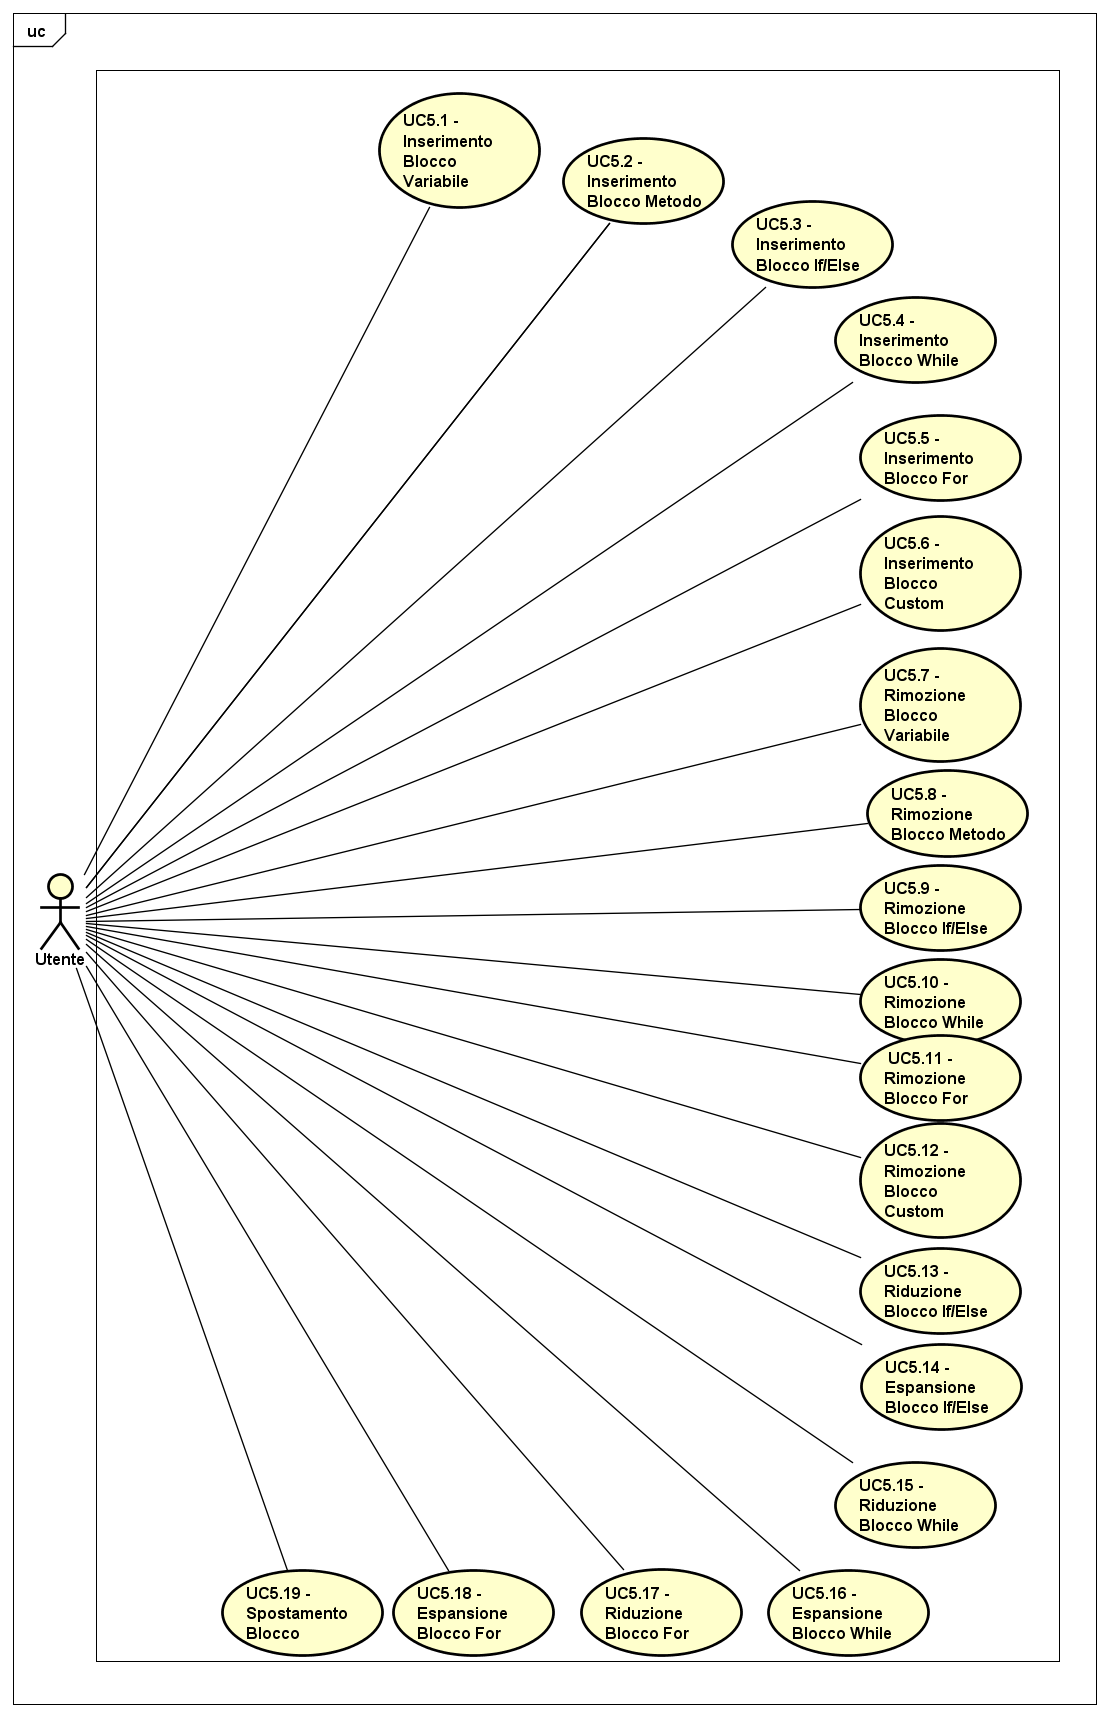
\includegraphics[width=1\textwidth]{Diagrammi casi d'uso/UC5 - Realizzazione Diagramma delle Attivita}
%	}
%	\caption{UC5 - Realizzazione Diagramma delle Attività}
%\end{figure}
\begin{itemize}
	\item \textbf{Attori}: Utente;
	\item \textbf{Descrizione}: l'attore realizza e gestisce un diagramma delle attività per ogni metodo presente nel diagramma delle classi in modo tale da darne una implementazione più in dettaglio. Essa viene effettuata mediante blocchi specifici per ogni costrutto, per la gestione delle variabili e dei metodi. Tale diagramma quindi non è comforme allo standard UML;
	\item \textbf{Precondizione}: il sistema è passato dalla sezione dell'editor dedicata alla gestione del diagramma delle classi alla sezione dell'editor dedicata alla gestione del diagramma delle attività del metodo selezionato;
	\item \textbf{Postcondizione}: il sistema visualizza il diagramma delle attività del metodo selezionato come realizzato dall'utente del programma;
	\item \textbf{Scenario principale}:
	\begin{enumerate}
		\item l'attore può inserire un blocco variabile (UC5.1);
		\item l'attore può inserire un blocco metodo (UC5.2);
		\item l'attore può inserire un blocco if/else (UC5.3);
		\item l'attore può inserire un blocco while (UC5.4);
		\item l'attore può inserire un blocco for (UC5.5);
		\item l'attore può inserire un blocco custom (UC5.6);
		\item l'attore può rimuovere un blocco variabile (UC5.7);
		\item l'attore può rimuovere un blocco metodo (UC5.8);
		\item l'attore può rimuovere un blocco if/else (UC5.9);
		\item l'attore può rimuovere  un blocco while (UC5.10);
		\item l'attore può rimuovere un blocco for (UC5.11);
		\item l'attore può rimuovere un blocco custom (UC5.12);
		\item l'attore può ridurre un blocco if/else (UC5.13);
		\item l'attore può espandere un blocco if/else (UC5.14);
		\item l'attore può ridurre un blocco while (UC5.15);
		\item l'attore può espandere un blocco while (UC5.16);
		\item l'attore può ridurre un blocco for (UC5.17);
		\item l'attore può espandere un blocco for (UC5.18);
		\item l'attore può spostare un qualsiasi blocco già inserito (UC5.19);
		\item l'attore può modificare un blocco variabile (UC5.20);
		\item l'attore può modificare un blocco metodo (UC5.21);
		\item l'attore può modificare un blocco if/else (UC5.22);
		\item l'attore può modificare un blocco while (UC5.23);
		\item l'attore può modificare un blocco for (UC5.24);
		\item l'attore può modificare un blocco custom (UC5.25);
		\item l'attore può inserire un blocco return (UC5.26).
	\end{enumerate}
\end{itemize}

\subsubsection{UC5.1: Inserimento Blocco Variabile}
\label{UC5.1}
\myimg{UC5.1 - Inserimento Blocco Variabile}
\begin{itemize}
	\item \textbf{Attori}: Utente;
	\item \textbf{Descrizione}: l'attore può inserire un blocco variabile scegliendo tra un blocco variabile di inizializzazione e un blocco variabile di assegnazione;
	\item \textbf{Precondizione}: il sistema, nella sezione dell'editor dedicata alla gestione del diagramma delle attività, visualizza un diagramma delle attività (eventualmente vuoto) associato ad un particolare metodo;
	\item \textbf{Postcondizione}: il sistema visualizza il blocco inserito mostrando eventualmente il commento specificato dall'attore e posizionandolo successivamente all'ultimo blocco generico precedentemente inserito nel diagramma delle attività corrente;
	\item \textbf{Scenario principale}:
	\begin{enumerate}
		\item l'attore può scegliere di creare e inizializzare una variabile (UC5.1.1);
		\item l'attore può scegliere di assegnare un valore ad una variabile esistente da scegliere (UC5.1.2);
		\item l'attore può scegliere di inserire un commento (UC5.1.3);
		\item l'attore può confermare l'inserimento del blocco variabile (UC5.1.4).
	\end{enumerate}
\end{itemize}

\paragraph{UC5.1.1: Inizializzazione Variabile}
\label{UC5.1.1}
\begin{itemize}
	\item \textbf{Attori}: Utente;
	\item \textbf{Descrizione}: l'attore può creare ed inizializzare una variabile assegnandole un valore;
	\item \textbf{Precondizione}: l'attore ha selezionato un blocco di inizializzazione variabile da inserire e il sistema visualizza il relativo form per l'inserimento dei dati;
	\item \textbf{Postcondizione}: il sistema ha ricevuto il dato richiesto;
	\item \textbf{Scenario principale}: l'attore deve indicare il nome e il tipo della variabile da creare ed eventualmente un valore da assegnarle: tale valore può essere anche ritornato da un metodo che può essere scelto tra quelli proposti.
\end{itemize}

\paragraph{UC5.1.2: Assegnazione Variabile}
\label{UC5.1.2}
\begin{itemize}
	\item \textbf{Attori}: Utente;
	\item \textbf{Descrizione}: l'attore può assegnare un valore ad una variabile esistente e visibile;
	\item \textbf{Precondizione}: l'attore ha selezionato un blocco di assegnazione variabile da inserire e il sistema visualizza il relativo form per l'inserimento dei dati;
	\item \textbf{Postcondizione}: il sistema ha ricevuto il dato richiesto;
	\item \textbf{Scenario principale}: l'attore deve fornire un valore da assegnare ad una variabile esistente e visibile: tale valore può essere anche ritornato da un metodo che può essere scelto tra quelli proposti.
\end{itemize}

\paragraph{UC5.1.3: Inserimento Commento Blocco Variabile}
\label{UC5.1.3}
\begin{itemize}
	\item \textbf{Attori}: Utente;
	\item \textbf{Descrizione}: l'attore deve inserire un commento per il blocco variabile selezionato;
	\item \textbf{Precondizione}: l'attore ha selezionato un blocco di assegnazione variabile da inserire e il sistema visualizza il relativo form per l'inserimento dei dati;
	\item \textbf{Postcondizione}: il sistema ha ricevuto il dato richiesto;
	\item \textbf{Scenario principale}: l'attore inserisce un commento per il blocco variabile selezionato.
\end{itemize}

\paragraph{UC5.1.4: Conferma Inserimento Blocco Variabile}
\label{UC5.1.4}
\begin{itemize}
	\item \textbf{Attori}: Utente;
	\item \textbf{Descrizione}: l'attore può confermare l'inserimento del blocco variabile selezionato;
	\item \textbf{Precondizione}: l'attore ha selezionato un blocco di assegnazione variabile da inserire e il sistema visualizza il relativo form per l'inserimento dei dati;
	\item \textbf{Postcondizione}: il sistema visualizza il blocco variabile inserito posizionandolo successivamente all'ultimo blocco generico precedentemente inserito nel diagramma delle attività corrente;
	\item \textbf{Scenario principale}: l'attore conferma l'inserimento del blocco variabile selezionato;
	\item \textbf{Estensioni}: l'attore visualizza un messaggio d'errore sull'inserimento dei dati (UC5.1.4.1);
	\item \textbf{Scenari alternativi}:
	\begin{itemize}
		\item l'attore non ha indicato il nome della variabile da inizializzare;
		\item l'attore non ha fornito un valore da assegnare alla variabile già esistente e visibile;
		\item l'attore non ha inserito un commento.
	\end{itemize}
\end{itemize}

\subparagraph{UC5.1.4.1: Visualizzazione Errore Inserimento Blocco Variabile}
\label{UC5.1.4.1}
\begin{itemize}
	\item \textbf{Attori}: Utente;
	\item \textbf{Descrizione}: l'attore può visualizzare un messaggio d'errore in corrispondenza della conferma di inserimento nel caso si siano verificati uno o più scenari alternativi durante la fase di inserimento di un blocco variabile;
	\item \textbf{Precondizione}: il sistema non ha ricevuto sufficienti informazioni per l'inserimento di un blocco variabile;
	\item \textbf{Postcondizione}: il sistema avvisa l'attore dell'errore verificatosi, tramite un opportuno messaggio;
	\item \textbf{Scenario principale}: l'attore visualizza un messaggio d'errore.
\end{itemize}

\subsubsection{UC5.2: Inserimento Blocco Metodo}
\label{UC5.2}
\myimg{UC5.2 - Inserimento Blocco Metodo}
\begin{itemize}
	\item \textbf{Attori}: Utente;
	\item \textbf{Descrizione}: l'attore può inserire un blocco metodo allo scopo di inserire all'interno del diagramma la chiamata ad un particolare metodo definito altrove (eventualmente nel corrispondente diagramma delle classi);
	\item \textbf{Precondizione}: il sistema, nella sezione dell'editor dedicata alla gestione del diagramma delle attività, visualizza un diagramma delle attività (eventualmente vuoto) associato ad un particolare metodo;
	\item \textbf{Postcondizione}: il sistema visualizza il blocco inserito mostrando eventualmente il commento specificato dall'attore e posizionandolo successivamente all'ultimo blocco generico precedentemente inserito nel diagramma delle attività corrente;
	\item \textbf{Scenario principale}:
	\begin{enumerate}
		\item l'attore può scegliere di inserire un metodo (UC5.2.1);
		\item l'attore può scegliere di inserire un commento (UC5.2.2);
		\item l'attore può confermare l'inserimento del blocco metodo (UC5.2.3).
	\end{enumerate}
\end{itemize}

\paragraph{UC5.2.1: Chiamata di Metodo}
\label{UC5.2.1}
\begin{itemize}
	\item \textbf{Attori}: Utente;
	\item \textbf{Descrizione}: l'attore deve invocare un metodo da inserire all'interno del blocco tra quelli disponibili;
	\item \textbf{Precondizione}: l'attore ha selezionato un blocco metodo da inserire e il sistema visualizza il form per l'inserimento dei dati;
	\item \textbf{Postcondizione}: il sistema ha ricevuto il dato richiesto;
	\item \textbf{Scenario principale}: l'attore deve scegliere un metodo da invocare tra quelli proposti.
\end{itemize}

\paragraph{UC5.2.2: Inserimento Commento Blocco Metodo}
\label{UC5.2.2}
\begin{itemize}
	\item \textbf{Attori}: Utente;
	\item \textbf{Descrizione}: l'attore deve inserire un commento per il blocco metodo da inserirsi;
	\item \textbf{Precondizione}: l'attore ha selezionato un blocco metodo da inserire e il sistema visualizza il form per l'inserimento dei dati;
	\item \textbf{Postcondizione}: il sistema ha ricevuto il dato richiesto;
	\item \textbf{Scenario principale}: l'attore inserisce un commento per il blocco metodo selezionato.
\end{itemize}

\paragraph{UC5.2.3: Conferma Inserimento Blocco Metodo}
\label{UC5.2.3}
\begin{itemize}
	\item \textbf{Attori}: Utente;
	\item \textbf{Descrizione}: l'attore può confermare l'inserimento del blocco metodo;
	\item \textbf{Precondizione}: l'attore ha selezionato un blocco metodo da inserire e il sistema visualizza il form per l'inserimento dei dati;
	\item \textbf{Postcondizione}: il sistema visualizza il blocco metodo inserito posizionandolo successivamente all'ultimo blocco generico precedentemente inserito nel diagramma delle attività corrente;	
	\item \textbf{Scenario principale}: l'attore conferma l'inserimento del blocco metodo;
	\item \textbf{Estensioni}: l'attore visualizza un messaggio d'errore sull'inserimento dei dati (UC5.2.3.1);
	\item \textbf{Scenari alternativi}:
	\begin{itemize}
		\item l'attore non ha indicato un metodo da inserire;
		\item l'attore non ha inserito un commento a corredo del blocco metodo.
	\end{itemize}
\end{itemize}

\subparagraph{UC5.2.3.1: Visualizzazione Errore Inserimento Blocco Metodo}
\label{UC5.2.3.1}
\begin{itemize}
	\item \textbf{Attori}: Utente;
	\item \textbf{Descrizione}: l'attore può visualizzare un messaggio d'errore in corrispondenza della conferma di inserimento nel caso si siano verificati uno o più scenari alternativi durante la fase di inserimento di un blocco metodo;
	\item \textbf{Precondizione}: il sistema non ha ricevuto sufficienti informazioni per l'inserimento di un blocco metodo;
	\item \textbf{Postcondizione}: il sistema avvisa l'attore dell'errore verificatosi, tramite un opportuno messaggio;
	\item \textbf{Scenario principale}: l'attore visualizza un messaggio d'errore.
\end{itemize}

\subsubsection{UC5.3: Inserimento Blocco If/Else}
\label{UC5.3}
\myimg{UC5.3 - Inserimento Blocco If_Else}
\begin{itemize}
	\item \textbf{Attori}: Utente;
	\item \textbf{Descrizione}: l'attore può inserire un blocco if/else e in caso voglia indicare semplicemente la condizione di if senza andare a specificare quella antitetica, sarà per lui sufficiente lasciare vuoto il corpo del blocco else;
	\item \textbf{Precondizione}: il sistema, nella sezione dell'editor dedicata alla gestione del diagramma delle attività, visualizza un diagramma delle attività (eventualmente vuoto) associato ad un particolare metodo;
	\item \textbf{Postcondizione}: il sistema visualizza il blocco inserito mostrando il commento inserito dall'attore a corredo e posizionandolo successivamente all'ultimo blocco generico precedentemente inserito nel diagramma delle attività corrente;
	\item \textbf{Scenario principale}:
	\begin{enumerate}
		\item l'attore può scegliere di inserire la condizione da verificare (UC5.3.1);
		\item l'attore può scegliere di inserire il contenuto del blocco if (UC5.3.2);
		\item l'attore può scegliere di inserire il contenuto del blocco else (UC5.3.3);
		\item l'attore può scegliere di inserire un commento (UC5.3.4);
		\item l'attore può confermare l'inserimento del blocco if/else (UC5.3.5).
	\end{enumerate}
\end{itemize}

\paragraph{UC5.3.1: Condizione Blocco If}
\label{UC5.3.1}
\begin{itemize}
	\item \textbf{Attori}: Utente;
	\item \textbf{Descrizione}: l'attore può inserire la condizione da verificare del blocco if; da inserire e il sistema visualizza il relativo form per l'inserimento dei dati;
	\item \textbf{Postcondizione}: il sistema ha ricevuto il dato richiesto;
	\item \textbf{Scenario principale}:
	\item \textbf{Precondizione}: l'attore ha selezionato un blocco if
	l'attore deve inserire la condizione da verificare del blocco if come espressione booleana espressa con il linguaggio target di generazione del codice dell'applicazione.
\end{itemize}

\paragraph{UC5.3.2: Corpo Blocco If}
\label{UC5.3.2}
\begin{itemize}
	\item \textbf{Attori}: Utente;
	\item \textbf{Descrizione}: l'attore può inserire una serie di blocchi tra quelli resi disponibili dall'editor per descrivere il comportamento del corpo del blocco if stesso;
	\item \textbf{Precondizione}: l'attore ha selezionato un blocco if da inserire e il sistema visualizza il relativo form per l'inserimento dei dati;
	\item \textbf{Postcondizione}: il sistema ha ricevuto il dato richiesto;
	\item \textbf{Scenario principale}: l'attore deve inserire uno o più blocchi tra quelli resi disponibili dall'editor.
\end{itemize}

\paragraph{UC5.3.3: Corpo Blocco Else}
\label{UC5.3.3}
\begin{itemize}
	\item \textbf{Attori}: Utente;
	\item \textbf{Descrizione}: l'attore può inserire una serie di blocchi tra quelli resi disponibili dall'editor per descrivere il comportamento del corpo del blocco else stesso;
	\item \textbf{Precondizione}: l'attore ha selezionato un blocco if da inserire e il sistema visualizza il relativo form per l'inserimento dei dati;
	\item \textbf{Postcondizione}: il sistema ha ricevuto il dato richiesto;
	\item \textbf{Scenario principale}: l'attore deve inserire uno o più blocchi tra quelli resi disponibili dall'editor.
\end{itemize}

\paragraph{UC5.3.4: Inserimento Commento Blocco If/Else}
\label{UC5.3.4}
\begin{itemize}
	\item \textbf{Attori}: Utente;
	\item \textbf{Descrizione}: l'attore deve inserire un commento per il blocco if/else;
	\item \textbf{Precondizione}: l'attore ha selezionato un blocco if da inserire e il sistema visualizza il relativo form per l'inserimento dei dati;
	\item \textbf{Postcondizione}: il sistema ha ricevuto il dato richiesto;
	\item \textbf{Scenario principale}: l'attore inserisce un commento per il blocco if/else.
\end{itemize}

\paragraph{UC5.3.5: Conferma Inserimento Blocco If/Else}
\label{UC5.3.5}
\begin{itemize}
	\item \textbf{Attori}: Utente;
	\item \textbf{Descrizione}: l'attore può confermare l'inserimento del blocco if/else;
	\item \textbf{Precondizione}: l'attore ha selezionato un blocco if da inserire e il sistema visualizza il relativo form per l'inserimento dei dati;
	\item \textbf{Postcondizione}: il sistema visualizza il blocco if/else inserito posizionandolo successivamente all'ultimo blocco generico precedentemente inserito nel diagramma delle attività corrente;
	\item \textbf{Scenario principale}: l'attore conferma l'inserimento del blocco if/else selezionato;
	\item \textbf{Estensioni}: l'attore visualizza un messaggio d'errore sull'inserimento dei dati (UC5.3.5.1);
	\item \textbf{Scenari alternativi}:
	\begin{itemize}
		\item l'attore non ha fornito la condizione da verificare;
		\item l'attore non ha inserito un commento.
	\end{itemize}
\end{itemize}

\subparagraph{UC5.3.5.1: Visualizzazione Errore Inserimento Blocco If/Else}
\label{UC5.3.5.1}
\begin{itemize}
	\item \textbf{Attori}: Utente;
	\item \textbf{Descrizione}: l'attore può visualizzare un messaggio d'errore in corrispondenza della conferma di inserimento nel caso si siano verificati uno o più scenari alternativi durante la fase di inserimento di un blocco if/else;
	\item \textbf{Precondizione}: il sistema non ha ricevuto sufficienti informazioni per l'inserimento di un blocco if/else;
	\item \textbf{Postcondizione}: il sistema avvisa l'attore dell'errore verificatosi, tramite un opportuno messaggio;
	\item \textbf{Scenario principale}: l'attore visualizza un messaggio d'errore.
\end{itemize}

\subsubsection{UC5.4: Inserimento Blocco While}
\label{UC5.4}
\myimg{UC5.4 - Inserimento Blocco While}
\begin{itemize}
	\item \textbf{Attori}: Utente;
	\item \textbf{Descrizione}: l'attore può inserire un blocco while specificandone condizione e istruzioni del corrispondente corpo di codice;
	\item \textbf{Precondizione}: il sistema, nella sezione dell'editor dedicata alla gestione del diagramma delle attività, visualizza un diagramma delle attività (eventualmente vuoto) associato ad un particolare metodo;
	\item \textbf{Postcondizione}: il sistema visualizza il blocco inserito mostrando il commento inserito dall'attore e posizionandolo successivamente all'ultimo blocco generico precedentemente inserito nel diagramma delle attività corrente;
	\item \textbf{Scenario principale}:
	\begin{enumerate}
		\item l'attore può scegliere di inserire la condizione da verificare (UC5.4.1);
		\item l'attore può scegliere di inserire il corpo del blocco while (UC5.4.2);
		\item l'attore può scegliere di inserire un commento (UC5.4.3);
		\item l'attore può confermare l'inserimento del blocco while (UC5.4.4).
	\end{enumerate}
\end{itemize}

\paragraph{UC5.4.1: Condizione Blocco While}
\label{UC5.4.1}
\begin{itemize}
	\item \textbf{Attori}: Utente;
	\item \textbf{Descrizione}: l'attore può inserire la condizione da verificare del blocco while;
	\item \textbf{Precondizione}: l'attore ha selezionato un blocco while da inserire e il sistema visualizza il relativo form per l'inserimento dei dati;
	\item \textbf{Postcondizione}: il sistema ha ricevuto il dato richiesto;
	\item \textbf{Scenario principale}: l'attore deve inserire la condizione da verificare del blocco while come espressione booleana espressa con il linguaggio target di generazione del codice dell'applicazione.
\end{itemize}

\paragraph{UC5.4.2: Corpo Blocco While}
\label{UC5.4.2}
\begin{itemize}
	\item \textbf{Attori}: Utente;
	\item \textbf{Descrizione}: l'attore può inserire uno o più blocchi tra quelli resi disponibili dall'editor per descrivere il comportamento del corpo del blocco while stesso;
	\item \textbf{Precondizione}: l'attore ha selezionato un blocco while da inserire e il sistema visualizza il relativo form per l'inserimento dei dati;
	\item \textbf{Postcondizione}: il sistema ha ricevuto il dato richiesto;
	\item \textbf{Scenario principale}: l'attore deve inserire uno o più blocchi tra quelli resi disponibili dall'editor.
\end{itemize}

\paragraph{UC5.4.3: Inserimento Commento Blocco While}
\label{UC5.4.3}
\begin{itemize}
	\item \textbf{Attori}: Utente;
	\item \textbf{Descrizione}: l'attore deve inserire un commento per il blocco while;
	\item \textbf{Precondizione}: l'attore ha selezionato un blocco while da inserire e il sistema visualizza il relativo form per l'inserimento dei dati;
	\item \textbf{Postcondizione}: il sistema ha ricevuto il dato richiesto;
	\item \textbf{Scenario principale}: l'attore inserisce un commento per il blocco while.
\end{itemize}

\paragraph{UC5.4.4: Conferma Inserimento Blocco While}
\label{UC5.4.4}
\begin{itemize}
	\item \textbf{Attori}: Utente;
	\item \textbf{Descrizione}: l'attore può confermare l'inserimento del blocco while;
	\item \textbf{Precondizione}: l'attore ha selezionato un blocco while da inserire e il sistema visualizza il relativo form per l'inserimento dei dati;
	\item \textbf{Postcondizione}: il sistema visualizza il blocco while inserito posizionandolo successivamente all'ultimo blocco generico precedentemente inserito nel diagramma delle attività corrente;
	\item \textbf{Scenario principale}: l'attore conferma l'inserimento del blocco while;
	\item \textbf{Estensioni}: l'attore visualizza un messaggio d'errore sull'inserimento dei dati (UC5.4.4.1);
	\item \textbf{Scenari alternativi}:
	\begin{itemize}
		\item l'attore non ha fornito la condizione da verificare;
		\item l'attore non ha inserito un commento.
	\end{itemize}
\end{itemize}

\subparagraph{UC5.4.4.1: Visualizzazione Errore Inserimento Blocco While}
\label{UC5.4.4.1}
\begin{itemize}
	\item \textbf{Attori}: Utente;
	\item \textbf{Descrizione}: l'attore può visualizzare un messaggio d'errore in corrispondenza della conferma di inserimento nel caso si fossero verificati uno o più scenari alternativi durante la fase di inserimento di un blocco while;
	\item \textbf{Precondizione}: il sistema non ha ricevuto sufficienti informazioni per l'inserimento di un blocco while;
	\item \textbf{Postcondizione}: il sistema avvisa l'attore dell'errore verificatosi, tramite un opportuno messaggio;
	\item \textbf{Scenario principale}: l'attore visualizza un messaggio d'errore.
\end{itemize}

\subsubsection{UC5.5: Inserimento Blocco For}
\label{UC5.5}
\myimg{UC5.5 - Inserimento Blocco For}
\begin{itemize}
	\item \textbf{Attori}: Utente;
	\item \textbf{Descrizione}: l'attore può inserire un blocco for specificandone condizione, passo e le istruzioni che andranno a comporre il relativo corpo di codice;
	\item \textbf{Precondizione}: il sistema, nella sezione dell'editor dedicata alla gestione del diagramma delle attività, visualizza un diagramma delle attività (eventualmente vuoto) associato ad un particolare metodo;
	\item \textbf{Postcondizione}: il sistema visualizza il blocco inserito mostrando il commento inserito dall'attore e posizionandolo successivamente all'ultimo blocco generico precedentemente
	inserito nel diagramma delle attività corrente;
	\item \textbf{Scenario principale}:
	\begin{enumerate}
		\item l'attore può scegliere di inserire il codice di inizializzazione (UC5.5.1);
		\item l'attore può scegliere di inserire la condizione da verificare (UC5.5.2);
		\item l'attore può scegliere di inserire il passo di incremento/decremento (UC5.5.3);
		\item l'attore può scegliere di inserire il corpo del for (UC5.5.4);
		\item l'attore può scegliere di inserire un commento (UC5.5.5);
		\item l'attore può confermare l'inserimento del blocco for (UC5.5.6).
	\end{enumerate}
\end{itemize}

\paragraph{UC5.5.1: Inizializzazione Blocco For}
\label{UC5.5.1}
\begin{itemize}
	\item \textbf{Attori}: Utente;
	\item \textbf{Descrizione}: l'attore può inserire l'inizializzazione del blocco for;
	\item \textbf{Precondizione}: l'attore ha selezionato un blocco for da inserire e il sistema visualizza il relativo form per l'inserimento dei dati;
	\item \textbf{Postcondizione}: il sistema ha ricevuto il dato richiesto;
	\item \textbf{Scenario principale}: l'attore deve inserire l'inizializzazione del blocco for creando ed inizializzando una variabile o scegliendone una tra quelle disponibili.
\end{itemize}

\paragraph{UC5.5.2: Condizione Blocco For}
\label{UC5.5.2}
\begin{itemize}
	\item \textbf{Attori}: Utente;
	\item \textbf{Descrizione}: l'attore può inserire la condizione da verificare all'interno blocco for;
	\item \textbf{Precondizione}: l'attore ha selezionato un blocco for da inserire e il sistema visualizza il relativo form per l'inserimento dei dati;
	\item \textbf{Postcondizione}: il sistema ha ricevuto il dato richiesto;
	\item \textbf{Scenario principale}: l'attore deve inserire la condizione da verificare del blocco for come espressione booleana espressa con il linguaggio target di generazione del codice dell'applicazione.
\end{itemize}

\paragraph{UC5.5.3: Incremento/Decremento Blocco For}
\label{UC5.5.3}
\begin{itemize}
	\item \textbf{Attori}: Utente;
	\item \textbf{Descrizione}: l'attore può inserire il passo di incremento/decremento del blocco for;
	\item \textbf{Precondizione}: l'attore ha selezionato un blocco for da inserire e il sistema visualizza il relativo form per l'inserimento dei dati;
	\item \textbf{Postcondizione}: il sistema ha ricevuto il dato richiesto;
	\item \textbf{Scenario principale}: l'attore deve inserire il passo di incremento/decremento del blocco for scegliendo una variabile tra quelle disponibili e visibili.
\end{itemize}

\paragraph{UC5.5.4: Corpo Blocco For}
\label{UC5.5.4}
\begin{itemize}
	\item \textbf{Attori}: Utente;
	\item \textbf{Descrizione}: l'attore può inserire uno o più blocchi tra quelli resi disponibili dall'editor per descrivere il comportamento del corpo del blocco for stesso;
	\item \textbf{Precondizione}: l'attore ha selezionato un blocco for da inserire e il sistema visualizza il relativo form per l'inserimento dei dati;
	\item \textbf{Postcondizione}: il sistema ha ricevuto il dato richiesto;
	\item \textbf{Scenario principale}: l'attore deve inserire uno o più blocchi tra quelli resi disponibili dall'editor.
\end{itemize}

\paragraph{UC5.5.5: Inserimento Commento Blocco For}
\label{UC5.5.5}
\begin{itemize}
	\item \textbf{Attori}: Utente;
	\item \textbf{Descrizione}: l'attore deve inserire un commento per il blocco for;
	\item \textbf{Precondizione}: l'attore ha selezionato un blocco for da inserire e il sistema visualizza il relativo form per l'inserimento dei dati;
	\item \textbf{Postcondizione}: il sistema ha ricevuto il dato richiesto;
	\item \textbf{Scenario principale}: l'attore inserisce un commento per il blocco for.
\end{itemize}

\paragraph{UC5.5.6: Conferma Inserimento Blocco For}
\label{UC5.5.6}
\begin{itemize}
	\item \textbf{Attori}: Utente;
	\item \textbf{Descrizione}: l'attore può confermare l'inserimento del blocco for;
	\item \textbf{Precondizione}: l'attore ha selezionato un blocco for da inserire e il sistema visualizza il relativo form per l'inserimento dei dati;
	\item \textbf{Postcondizione}: il sistema visualizza il blocco for inserito posizionandolo successivamente all'ultimo blocco generico precedentemente inserito nel diagramma delle attività corrente;
	\item \textbf{Scenario principale}: l'attore conferma l'inserimento del blocco for;
	\item \textbf{Estensioni}: l'attore visualizza un messaggio d'errore sull'inserimento dei dati (UC5.5.6.1);
	\item \textbf{Scenari alternativi}:
	\begin{itemize}
		\item l'attore non ha fornito la condizione da verificare;
		\item l'attore non ha fornito l'incremento/decremento;
		\item l'attore non ha inserito un commento.
	\end{itemize}
\end{itemize}

\subparagraph{UC5.5.6.1: Visualizzazione Errore Inserimento Blocco For}
\label{UC5.5.6.1}
\begin{itemize}
	\item \textbf{Attori}: Utente;
	\item \textbf{Descrizione}: l'attore può visualizzare un messaggio d'errore in corrispondenza della conferma di inserimento nel caso si fossero verificati uno o più scenari alternativi durante la fase di inserimento di un blocco for;
	\item \textbf{Precondizione}: il sistema non ha ricevuto sufficienti informazioni per l'inserimento di un blocco for;
	\item \textbf{Postcondizione}: il sistema avvisa l'attore dell'errore verificatosi, tramite un opportuno messaggio;
	\item \textbf{Scenario principale}: l'attore visualizza un messaggio d'errore.
\end{itemize}

\subsubsection{UC5.6: Inserimento Blocco Custom}
\label{UC5.6}
\myimg{UC5.6 - Inserimento Blocco Custom}
\begin{itemize}
	\item \textbf{Attori}: Utente;
	\item \textbf{Descrizione}: l'attore può inserire un blocco custom di codice all'interno del quale inserire liberamente uno o più \gloss{statement} nel linguaggio target di generazione di codice dell'editor;
	\item \textbf{Precondizione}: il sistema, nella sezione dell'editor dedicata alla gestione del diagramma delle attività, visualizza un diagramma delle attività (eventualmente vuoto) associato ad un particolare metodo;
	\item \textbf{Postcondizione}: il sistema visualizza il blocco inserito mostrando il commento inserito dall'attore e posizionandolo successivamente all'ultimo blocco generico precedentemente
	inserito nel diagramma delle attività corrente;
	\item \textbf{Scenario principale}:
	\begin{enumerate}
		\item l'attore può inserisce il contenuto in codice del blocco custom (UC5.6.1);
		\item l'attore può inserisce un commento relativo al blocco custom(UC5.6.2);
		\item l'attore può confermare l'inserimento del blocco custom (UC5.6.3).
	\end{enumerate}
\end{itemize}

\paragraph{UC5.6.1: Contenuto Blocco Custom}
\label{UC5.6.1}
\begin{itemize}
	\item \textbf{Attori}: Utente;
	\item \textbf{Descrizione}: l'attore inserisce il contenuto in codice del blocco custom;
	\item \textbf{Precondizione}: l'attore ha selezionato un blocco custom da inserire e il sistema visualizza il form per l'inserimento dei dati;
	\item \textbf{Postcondizione}: il sistema ha ricevuto il dato richiesto;
	\item \textbf{Scenario principale}: l'attore deve inserire il contenuto in codice del blocco custom in Java, il linguaggio target di generazione del codice dell'applicativo.
\end{itemize}

\paragraph{UC5.6.2: Inserimento Commento Blocco Custom}
\label{UC5.6.2}
\begin{itemize}
	\item \textbf{Attori}: Utente;
	\item \textbf{Descrizione}: l'attore deve inserire un commento per il blocco custom;
	\item \textbf{Precondizione}: l'attore ha selezionato un blocco custom da inserire e il sistema visualizza il form per l'inserimento dei dati;
	\item \textbf{Postcondizione}: il sistema ha ricevuto il dato richiesto;
	\item \textbf{Scenario principale}: l'attore inserisce un commento per il blocco custom che ne illustri il principale comportamento.
\end{itemize}

\paragraph{UC5.6.3: Conferma Inserimento Blocco Custom}
\label{UC5.6.3}
\begin{itemize}
	\item \textbf{Attori}: Utente;
	\item \textbf{Descrizione}: l'attore può confermare l'inserimento del blocco custom;
	\item \textbf{Precondizione}: il sistema visualizza il form per l'inserimento dei dati;
	\item \textbf{Postcondizione}: il sistema visualizza il blocco custom inserito;
	\item \textbf{Scenario principale}: l'attore conferma l'inserimento del blocco custom.
\end{itemize}

\subsubsection{UC5.7: Rimozione Blocco Variabile}
\label{UC5.7}
\begin{itemize}
	\item \textbf{Attori}: Utente;
	\item \textbf{Descrizione}: l'attore può rimuovere un blocco variabile;
	\item \textbf{Precondizione}: il sistema visualizza il blocco variabile precedentemente realizzato;
	\item \textbf{Postcondizione}: il sistema rimuove il blocco variabile;
	\item \textbf{Scenario principale}: l'attore rimuove il blocco variabile selezionato.
\end{itemize}

\subsubsection{UC5.8: Rimozione Blocco Metodo}
\label{UC5.8}
\begin{itemize}
	\item \textbf{Attori}: Utente;
	\item \textbf{Descrizione}: l'attore può rimuovere un blocco metodo;
	\item \textbf{Precondizione}: il sistema visualizza il blocco metodo precedentemente realizzato;
	\item \textbf{Postcondizione}: il sistema rimuove il blocco metodo;
	\item \textbf{Scenario principale}: l'attore rimuove il blocco metodo selezionato.
\end{itemize}

\subsubsection{UC5.9: Rimozione Blocco If/Else}
\label{UC5.9}
\begin{itemize}
	\item \textbf{Attori}: Utente;
	\item \textbf{Descrizione}: l'attore può rimuovere un blocco if/else;
	\item \textbf{Precondizione}: il sistema visualizza il blocco if/else precedentemente realizzato;
	\item \textbf{Postcondizione}: il sistema rimuove il blocco if/else;
	\item \textbf{Scenario principale}: l'attore rimuove il blocco if/else selezionato.
\end{itemize}

\subsubsection{UC5.10: Rimozione Blocco While}
\label{UC5.10}
\begin{itemize}
	\item \textbf{Attori}: Utente;
	\item \textbf{Descrizione}: l'attore può rimuovere un blocco while;
	\item \textbf{Precondizione}: il sistema visualizza il blocco while precedentemente realizzato;
	\item \textbf{Postcondizione}: il sistema rimuove il blocco while;
	\item \textbf{Scenario principale}: l'attore rimuove il blocco while selezionato.
\end{itemize}

\subsubsection{UC5.11: Rimozione Blocco For}
\label{UC5.11}
\begin{itemize}
	\item \textbf{Attori}: Utente;
	\item \textbf{Descrizione}: l'attore può rimuovere un blocco for;
	\item \textbf{Precondizione}: il sistema visualizza il blocco for precedentemente realizzato;
	\item \textbf{Postcondizione}: il sistema rimuove il blocco for;
	\item \textbf{Scenario principale}: l'attore rimuove il blocco for selezionato.
\end{itemize}

\subsubsection{UC5.12: Rimozione Blocco Custom}
\label{UC5.12}
\begin{itemize}
	\item \textbf{Attori}: Utente;
	\item \textbf{Descrizione}: l'attore può rimuovere un blocco custom;
	\item \textbf{Precondizione}: il sistema visualizza il blocco custom precedentemente realizzato;
	\item \textbf{Postcondizione}: il sistema rimuove il blocco custom;
	\item \textbf{Scenario principale}: l'attore rimuove il blocco custom selezionato.
\end{itemize}

\subsubsection{UC5.13: Riduzione Blocco If/Else}
\label{UC5.13}
\begin{itemize}
	\item \textbf{Attori}: Utente;
	\item \textbf{Descrizione}: l'attore può ridurre il blocco if/else;
	\item \textbf{Precondizione}: il sistema visualizza il blocco if/else precedentemente realizzato ed espanso;
	\item \textbf{Postcondizione}: il sistema visualizza il blocco if/else ridotto;
	\item \textbf{Scenario principale}: l'attore riduce il blocco if/else nascondendone il corpo.
\end{itemize}

\subsubsection{UC5.14: Espansione Blocco If/Else}
\label{UC5.14}
\begin{itemize}
	\item \textbf{Attori}: Utente;
	\item \textbf{Descrizione}: l'attore può espandere il blocco if/else;
	\item \textbf{Precondizione}: il sistema visualizza il blocco if/else precedentemente realizzato e ridotto;
	\item \textbf{Postcondizione}: il sistema visualizza il blocco if/else espanso;
	\item \textbf{Scenario principale}: l'attore espande il blocco if/else mostrandone il corpo.
\end{itemize}

\subsubsection{UC5.15: Riduzione Blocco While}
\label{UC5.15}
\begin{itemize}
	\item \textbf{Attori}: Utente;
	\item \textbf{Descrizione}: l'attore può ridurre il blocco while;
	\item \textbf{Precondizione}: il sistema visualizza il blocco while precedentemente realizzato ed espanso;
	\item \textbf{Postcondizione}: il sistema visualizza il blocco while ridotto;
	\item \textbf{Scenario principale}: l'attore riduce il blocco while nascondendone il corpo.
\end{itemize}

\subsubsection{UC5.16: Espansione Blocco While}
\label{UC5.16}
\begin{itemize}
	\item \textbf{Attori}: Utente;
	\item \textbf{Descrizione}: l'attore può espandere il blocco while;
	\item \textbf{Precondizione}: il sistema visualizza il blocco while precedentemente realizzato e ridotto;
	\item \textbf{Postcondizione}: il sistema visualizza il blocco while espanso;
	\item \textbf{Scenario principale}: l'attore espande il blocco while mostrandone il corpo.
\end{itemize}

\subsubsection{UC5.17: Riduzione Blocco For}
\label{UC5.17}
\begin{itemize}
	\item \textbf{Attori}: Utente;
	\item \textbf{Descrizione}: l'attore può ridurre il blocco for;
	\item \textbf{Precondizione}: il sistema visualizza il blocco for precedentemente realizzato ed espanso;
	\item \textbf{Postcondizione}: il sistema visualizza il blocco for ridotto;
	\item \textbf{Scenario principale}: l'attore riduce il blocco for nascondendone il corpo.
\end{itemize}

\subsubsection{UC5.18: Espansione Blocco For}
\label{UC5.18}
\begin{itemize}
	\item \textbf{Attori}: Utente;
	\item \textbf{Descrizione}: l'attore può espandere il blocco for;
	\item \textbf{Precondizione}: il sistema visualizza il blocco for precedentemente realizzato e ridotto;
	\item \textbf{Postcondizione}: il sistema visualizza il blocco for espanso;
	\item \textbf{Scenario principale}: l'attore espande il blocco for mostrandone il corpo.
\end{itemize}

\subsubsection{UC5.19: Spostamento Blocco}
\label{UC5.19}
\begin{itemize}
	\item \textbf{Attori}: Utente;
	\item \textbf{Descrizione}: l'attore può spostare uno dei qualsiasi blocchi già inseriti modificandone la posizione all'interno del diagramma delle attività correntemente gestito;
	\item \textbf{Precondizione}: il sistema visualizza il diagramma delle attività correntemente gestito dall'attore ed in particolare il blocco che sarà selezionato per lo spostamento;
	\item \textbf{Postcondizione}: il sistema visualizza il blocco for nella nuova posizione specificata dall'utente;
	\item \textbf{Scenario principale}: l'attore muove il blocco selezionato in una nuova posizione del diagramma delle attività correntemente gestito.
\end{itemize}

% \item l'attore può modificare un blocco variabile (UC5.20);
\subsubsection{UC5.20: Modifica Blocco Variabile}
\label{UC5.20}
\myimg{UC5.20 - Modifica Blocco Variabile}
\begin{itemize}
	\item \textbf{Attori}: Utente;
	\item \textbf{Descrizione}: l'attore può modificare un blocco variabile;
	\item \textbf{Precondizione}: l'attore ha selezionato il blocco variabile da modificare e il sistema visualizza il form di inserimento dati ;
	\item \textbf{Postcondizione}: il sistema visualizza il blocco variabile modificato;
	\item \textbf{Scenario principale}:
	\begin{enumerate}
		\item l'attore può scegliere di modificare il nome della variabile (UC5.20.1);
		\item l'attore può scegliere di modificare il tipo della variabile (UC5.20.2);
		\item l'attore può scegliere di modificare il valore della variabile (UC5.20.3);
		\item l'attore può confermare le modifiche apportate al blocco variabile (UC5.20.4).
	\end{enumerate}
\end{itemize}

% \item l'attore può scegliere di modificare il nome della variabile (UC5.20.1);
\paragraph{UC5.20.1: Modifica Nome Variabile}
\label{UC5.20.1}
\begin{itemize}
	\item \textbf{Attori}: Utente;
	\item \textbf{Descrizione}: l'attore può modificare il nome della variabile selezionata per la modifica scegliendolo eventualmente fra quelli visibili nello scope in cui sta agendo;
	\item \textbf{Precondizione}: l'attore ha selezionato il blocco variabile da modificare e il sistema visualizza il form di inserimento dati ;
	\item \textbf{Postcondizione}: il form ha ricevuto i dati richiesti;
	\item \textbf{Scenario principale}: L'attore modifica il nome della variabile selezionata per la modifica.
\end{itemize}

% \item l'attore può scegliere di modificare il tipo della variabile (UC5.20.2);
\paragraph{UC5.20.2: Modifica Tipo Variabile}
\label{UC5.20.2}
\begin{itemize}
	\item \textbf{Attori}: Utente;
	\item \textbf{Descrizione}: l'attore può modificare il tipo della variabile selezionata per la modifica;
	\item \textbf{Precondizione}: l'attore ha selezionato il blocco variabile da modificare e il sistema visualizza il form di inserimento dati ;
	\item \textbf{Postcondizione}: il form ha ricevuto i dati richiesti;
	\item \textbf{Scenario principale}: L'attore modifica il tipo della variabile selezionata per la modifica.
	\end{itemize}
	% \item l'attore può scegliere di modificare il valore della variabile (UC5.20.3);
	\paragraph{UC5.20.3: Modifica Valore Variabile}
	\label{UC5.20.3}
	\begin{itemize}
		\item \textbf{Attori}: Utente;
		\item \textbf{Descrizione}: l'attore può modificare il valore della variabile selezionata per la modifica;
		\item \textbf{Precondizione}: l'attore ha selezionato il blocco variabile da modificare e il sistema visualizza il form di inserimento dati ;
		\item \textbf{Postcondizione}: il form ha ricevuto i dati richiesti;
		\item \textbf{Scenario principale}: L'attore modifica il valore della variabile selezionata per la modifica.
\end{itemize}

% \item l'attore può confermare le modifiche apportate al blocco variabile (UC5.20.4).
\paragraph{UC5.20.4: Conferma Modifica Blocco Variabile}
\label{UC5.20.4}
\begin{itemize}
	\item \textbf{Attori}: Utente;
	\item \textbf{Descrizione}: l'attore può confermare le modifiche apportate al blocco variabile selezionato per la modifica;
	\item \textbf{Precondizione}: l'attore ha selezionato il blocco variabile da modificare e il sistema visualizza il form di inserimento dati ;
	\item \textbf{Postcondizione}: il sistema visualizza il blocco variabile modificato;
	\item \textbf{Scenario principale}: L'attore conferma le modifiche apportate al blocco variabile.
	\item \textbf{Estensioni}: l'attore visualizza un messaggio d'errore sull'inserimento dei dati (UC5.1.4.1);
	\item \textbf{Scenari alternativi}:
	\begin{itemize}
		\item l'attore non ha indicato il nome della variabile da inizializzare;
		\item l'attore non ha fornito un valore da assegnare alla variabile già esistente e visibile;
		\item l'attore non ha inserito un commento.
	\end{itemize}
\end{itemize}

% \item l'attore può modificare un blocco metodo (UC5.21);
\subsubsection{UC5.21: Modifica Blocco Metodo}
\label{UC5.21}
\myimg{UC5.21 - Modifica Blocco Metodo}
\begin{itemize}
	\item \textbf{Attori}: Utente;\item \textbf{Scenario principale}:

	\item \textbf{Descrizione}: l'attore ha selezionato il blocco metodo da modificare e il sistema visualizza il form di inserimento dati ;
	\item \textbf{Postcondizione}: il sistema visualizza il blocco metodo modificato;
	\item \textbf{Scenario principale}:
	\begin{enumerate}
		\item l'attore può scegliere di modificare un metodo (UC5.21.1);
		\item l'attore può scegliere di modificare un commento (UC5.21.2);
		\item l'attore può confermare le modifiche apportate al blocco metodo (UC5.21.3).
	\end{enumerate}
\end{itemize}

% \item l'attore può scegliere di modificare un metodo (UC5.21.1);
\paragraph{UC5.21.1: Modifica Metodo}
\label{UC5.21.1}
\begin{itemize}
	\item \textbf{Attori}: Utente;
	\item \textbf{Descrizione}: l'attore può modificare il metodo selezionato per la modifica;
	\item \textbf{Precondizione}: l'attore ha selezionato il blocco metodo da modificare e il sistema visualizza il form di inserimento dati ;
	\item \textbf{Postcondizione}: il form ha ricevuto i dati richiesti;
	\item \textbf{Scenario principale}: L'attore modifica il blocco metodo selezionato per la modifica.
\end{itemize}

% \item l'attore può scegliere di modificare un commento (UC5.21.2);
\paragraph{UC5.21.2: Modifica Commento Metodo}
\label{UC5.21.2}
\begin{itemize}
	\item \textbf{Attori}: Utente;
	\item \textbf{Descrizione}: l'attore può modificare il commento relativo al blocco metodo selezionato per la modifica;
	\item \textbf{Precondizione}: l'attore ha selezionato il blocco metodo da modificare e il sistema visualizza il form di inserimento dati ;
	\item \textbf{Postcondizione}: il form ha ricevuto i dati richiesti;
	\item \textbf{Scenario principale}: L'attore modifica il commento del blocco metodo selezionato per la modifica.
\end{itemize}

% \item l'attore può confermare le modifiche apportate al blocco metodo (UC5.21.3).
\paragraph{UC5.21.3: Conferma Modifica Blocco Metodo}
\label{UC5.21.3}
\begin{itemize}
	\item \textbf{Attori}: Utente;
	\item \textbf{Descrizione}: l'attore può confermare le modifiche apportate al blocco metodo selezionato per la modifica;
	\item \textbf{Precondizione}: l'attore ha selezionato il blocco metodo da modificare e il sistema visualizza il form di inserimento dati ;
	\item \textbf{Postcondizione}: il sistema visualizza il blocco metodo modificato;
	\item \textbf{Scenario principale}: L'attore modifica  selezionata per la modifica.
	\item \textbf{Estensioni}: l'attore visualizza un messaggio d'errore sull'inserimento dei dati (UC5.2.3.1);
	\item \textbf{Scenari alternativi}:
	\begin{itemize}
		\item l'attore non ha indicato un metodo da inserire;
		\item l'attore non ha inserito un commento a corredo del blocco metodo.
	\end{itemize}
\end{itemize}

% \item l'attore può modificare un blocco if/else (UC5.22);
\subsubsection{UC5.22: Modifica Blocco If/Else}
\label{UC5.22}
\myimg{UC5.22 - Modifica Blocco If_Else}
\begin{itemize}
	\item \textbf{Attori}: Utente;
	\item \textbf{Descrizione}: l'attore può modificare il blocco if/else selezionato per la modifica;
	\item \textbf{Precondizione}: l'attore ha selezionato il blocco if/else da modificare e il sistema visualizza il form di inserimento dati ;
	\item \textbf{Postcondizione}: il sistema visualizza il blocco if/else modificato;
	\item \textbf{Scenario principale}:
	\begin{enumerate}
		\item l'attore può scegliere di modificare la condizione da verificare (UC5.22.1);
		\item l'attore può scegliere di modificare il commento (UC5.22.2);
		\item l'attore può confermare le modifiche apportate al blocco if/else (UC5.22.3).
	\end{enumerate}
\end{itemize}

% \item l'attore può scegliere di modificare la condizione da verificare (UC5.22.1);
\paragraph{UC5.22.1: Modifica Condizione Blocco If/Else}
\label{UC5.22.1}
\begin{itemize}
	\item \textbf{Attori}: Utente;
	\item \textbf{Descrizione}: l'attore può modificare la condizione da verificare relativa al blocco if/else selezionato per la modifica;
	\item \textbf{Precondizione}: l'attore ha selezionato il blocco if/else da modificare e il sistema visualizza il form di inserimento dati ;
	\item \textbf{Postcondizione}: il form ha ricevuto i dati richiesti;
	\item \textbf{Scenario principale}: L'attore modifica la condizione da verificare relativa al blocco if/else selezionato per la modifica.
\end{itemize}

% \item l'attore può scegliere di modificare il commento (UC5.22.2);
\paragraph{UC5.22.2: Modifica Contenuto Blocco If/Else}
\label{UC5.22.2}
\begin{itemize}
\item \textbf{Attori}: Utente;
	\item \textbf{Descrizione}: l'attore può modificare il commento relativo al blocco if/else selezionato per la modifica;
	\item \textbf{Precondizione}: l'attore ha selezionato il blocco if/else da modificare e il sistema visualizza il form di inserimento dati ;
	\item \textbf{Postcondizione}: il form ha ricevuto i dati richiesti;
	\item \textbf{Scenario principale}: L'attore modifica il commento relativo al blocco if/else selezionato per la modifica.
\end{itemize}

% \item l'attore può confermare le modifiche apportate al blocco if/else (UC5.22.3).
\paragraph{UC5.22.3: Conferma Modifica Blocco If/Else}
\label{UC5.22.3}
\begin{itemize}
	\item \textbf{Attori}: Utente;
	\item \textbf{Descrizione}: l'attore può confermare le modifiche apportate al blocco if/else selezionato per la modifica;
	\item \textbf{Precondizione}: l'attore ha selezionato il blocco if/else da modificare e il sistema visualizza il form di inserimento dati ;
	\item \textbf{Postcondizione}: il sistema visualizza il blocco if/else modificato;
	\item \textbf{Scenario principale}: L'attore conferma le modifiche apportate al blocco if/else selezionato per la modifica.
	\item \textbf{Estensioni}: l'attore visualizza un messaggio d'errore sull'inserimento dei dati (UC5.3.5.1);
	\item \textbf{Scenari alternativi}:
	\begin{itemize}
		\item l'attore non ha fornito la condizione da verificare;
		\item l'attore non ha inserito un commento.
	\end{itemize}
\end{itemize}

% \item l'attore può modificare un blocco while (UC5.23);
\subsubsection{UC5.23: Modifica Blocco While}
\label{UC5.23}
\myimg{UC5.23 - Modifica Blocco While}
\begin{itemize}
	\item \textbf{Attori}: Utente;
	\item \textbf{Descrizione}: l'attore può modificare il blocco while selezionato per la modifica;
	\item \textbf{Precondizione}: l'attore ha selezionato il blocco while e il sistema visualizza il form di inserimento dati ;
	\item \textbf{Postcondizione}: il sistema visualizza il blocco while modificato;
	\item \textbf{Scenario principale}:
	\begin{enumerate}
		\item l'attore può scegliere di modificare la condizione da verificare (UC5.23.1);
		\item l'attore può scegliere di inserire un commento (UC5.23.2);
		\item l'attore può confermare le modifiche apportate al blocco while (UC5.23.3).
	\end{enumerate}
\end{itemize}

% \item l'attore può scegliere di modificare la condizione da verificare (UC5.23.1);
\paragraph{UC5.23.1: Modifica Condizione Blocco While}
\label{UC5.23.1}
\begin{itemize}
	\item \textbf{Attori}: Utente;
	\item \textbf{Descrizione}: l'attore può modificare la condizione relativa al blocco while selezionato per la modifica;
	\item \textbf{Precondizione}: l'attore ha selezionato il blocco while da modificare e il sistema visualizza il form di inserimento dati ;
	\item \textbf{Postcondizione}: il form ha ricevuto i dati necessari;
	\item \textbf{Scenario principale}: L'attore modifica la condizione relativa al blocco while selezionato per la modifica.
\end{itemize}

% \item l'attore può scegliere di inserire un commento (UC5.23.2);
\paragraph{UC5.23.2: Modifica Commento Blocco While}
\label{UC5.23.2}
\begin{itemize}
	\item \textbf{Attori}: Utente;
	\item \textbf{Descrizione}: l'attore può modificare il commento relativo al blocco while selezionato per la modifica;
	\item \textbf{Precondizione}: l'attore ha selezionato il blocco while da modificare e il sistema visualizza il form di inserimento dati ;
	\item \textbf{Postcondizione}: il form ha ricevuto i dati necessari;
	\item \textbf{Scenario principale}: L'attore modifica il commento relativo al blocco while selezionato per la modifica.
\end{itemize}

% \item l'attore può confermare le modifiche apportate al blocco while (UC5.23.3).
\paragraph{UC5.23.3: Conferma Modifica Blocco While}
\label{UC5.23.3}
\begin{itemize}
	\item \textbf{Attori}: Utente;
	\item \textbf{Descrizione}: l'attore può confermare le modifiche apportate al blocco while selezionato per la modifica;
	\item \textbf{Precondizione}: l'attore ha selezionato il blocco while da modificare e il sistema visualizza il form di inserimento dati ;
	\item \textbf{Postcondizione}: il sistema visualizza il blocco while modificato;
	\item \textbf{Scenario principale}: L'attore conferma le modifiche apportate al blocco while selezionato per la modifica.
	\item \textbf{Estensioni}: l'attore visualizza un messaggio d'errore sull'inserimento dei dati (UC5.4.4.1);
	\item \textbf{Scenari alternativi}:
	\begin{itemize}
		\item l'attore non ha fornito la condizione da verificare;
		\item l'attore non ha inserito un commento.
	\end{itemize}
\end{itemize}

% \item l'attore può modificare un blocco for (UC5.24);
\subsubsection{UC5.24: Modifica Blocco For}
\label{UC5.24}
\myimg{UC5.24 - Modifica Blocco For}
\begin{itemize}
	\item \textbf{Attori}: Utente;
	\item \textbf{Descrizione}: l'attore può modificare il blocco for selezionato per la modifica;
	\item \textbf{Precondizione}: l'attore ha selezionato il blocco for e il sistema visualizza il form di inserimento dati ;
	\item \textbf{Postcondizione}: il sistema visualizza il blocco for modificato;
	\item \textbf{Scenario principale}:
	\begin{enumerate}
		\item l'attore può scegliere di modificare il codice di inizializzazione (UC5.24.1);
		\item l'attore può scegliere di modificare la condizione da verificare (UC5.24.2);
		\item l'attore può scegliere di modificare il passo di incremento/decremento (UC5.24.3);
		\item l'attore può scegliere di modificare un commento (UC5.24.4);
		\item l'attore può scegliere di confermare le modifiche apportate al blocco for (UC5.24.5).
	\end{enumerate}
\end{itemize}

% \item l'attore può scegliere di modificare il codice di inizializzazione (UC5.24.1);
\paragraph{UC5.24.1: Modifica Inizializzazione Blocco For}
\label{UC5.24.1}
\begin{itemize}
	\item \textbf{Attori}: Utente;
	\item \textbf{Descrizione}: l'attore può modificare l'inizializzazione del blocco for selezionato per la modifica;
	\item \textbf{Precondizione}: l'attore ha selezionato il blocco for da modificare e il sistema visualizza il form di inserimento dati ;
	\item \textbf{Postcondizione}: il form ha ricevuto i dati necessari;
	\item \textbf{Scenario principale}: L'attore modifica l'inizializzazione del blocco for selezionato per la modifica.
\end{itemize}

% \item l'attore può scegliere di modificare la condizione da verificare (UC5.24.2);
\paragraph{UC5.24.2: Modifica Condizione Blocco For}
\label{UC5.24.2}
\begin{itemize}
	\item \textbf{Attori}: Utente;
	\item \textbf{Descrizione}: l'attore può modificare la condizione del blocco for selezionato per la modifica;
	\item \textbf{Precondizione}: l'attore ha selezionato il blocco for da modificare e il sistema visualizza il form di inserimento dati ;
	\item \textbf{Postcondizione}: il form ha ricevuto i dati necessari;
	\item \textbf{Scenario principale}: L'attore modifica la condizione del blocco for selezionato per la modifica.
\end{itemize}

% \item l'attore può scegliere di modificare il passo di incremento/decremento (UC5.24.3);
\paragraph{UC5.24.3: Modifica Incremento/Decremento Blocco For}
\label{UC5.24.3}
\begin{itemize}
	\item \textbf{Attori}: Utente;
	\item \textbf{Descrizione}: l'attore può modificare il passo di incremento/decremento del blocco for selezionato per la modifica;
	\item \textbf{Precondizione}: l'attore ha selezionato il blocco for da modificare e il sistema visualizza il form di inserimento dati ;
	\item \textbf{Postcondizione}: il form ha ricevuto i dati necessari;
	\item \textbf{Scenario principale}: L'attore modifica il passo di incremento/decremento del blocco for selezionato per la modifica.
\end{itemize}

% \item l'attore può scegliere di modificare un commento (UC5.24.4);
\paragraph{UC5.24.4: Modifica Commento Blocco For}
\label{UC5.24.4}
\begin{itemize}
	\item \textbf{Attori}: Utente;
	\item \textbf{Descrizione}: l'attore può modificare il commento del blocco for selezionato per la modifica;
	\item \textbf{Precondizione}: l'attore ha selezionato il blocco for da modificare e il sistema visualizza il form di inserimento dati ;
	\item \textbf{Postcondizione}: il form ha ricevuto i dati necessari;
	\item \textbf{Scenario principale}: L'attore modifica il commento del blocco for selezionato per la modifica.
\end{itemize}

% \item l'attore può scegliere di confermare le modifiche apportate al blocco for (UC5.24.5).
\paragraph{UC5.24.5: Conferma Modifica Blocco For}
\label{UC5.24.5}
\begin{itemize}
	\item \textbf{Attori}: Utente;
	\item \textbf{Descrizione}: l'attore può confermare le modifiche apportate al blocco for selezionato per la modifica;
	\item \textbf{Precondizione}: l'attore ha selezionato il blocco for da modificare e il sistema visualizza il form di inserimento dati ;
	\item \textbf{Postcondizione}: il sistema visualizza il blocco for modificato;
	\item \textbf{Scenario principale}: L'attore conferma le modifiche apportate al blocco for selezionato per la modifica.
	\item \textbf{Estensioni}: l'attore visualizza un messaggio d'errore sull'inserimento dei dati (UC5.5.6.1);
	\item \textbf{Scenari alternativi}:
	\begin{itemize}
		\item l'attore non ha fornito la condizione da verificare;
		\item l'attore non ha fornito l'incremento/decremento;
		\item l'attore non ha inserito un commento.
	\end{itemize}
\end{itemize}

% \item l'attore può modificare un blocco custom (UC5.25).
\subsubsection{UC5.25: Modifica Blocco Custom}
\label{UC5.25}
\myimg{UC5.25 - Modifica Blocco Custom}
\begin{itemize}
	\item \textbf{Attori}: Utente;
	\item \textbf{Descrizione}: l'attore può modificare il blocco custom selezionato per la modifica;
	\item \textbf{Precondizione}: l'attore ha selezionato il blocco custom e il sistema visualizza il form di inserimento dati ;
	\item \textbf{Postcondizione}: il sistema visualizza il blocco custom modificato;
	\item \textbf{Scenario principale}:
	\begin{enumerate}
		\item l'attore può modificare il contenuto in codice del blocco custom (UC5.25.1);
		\item l'attore può modificare il commento relativo al blocco custom(UC5.25.2);
		\item l'attore può confermare le modifiche apportate al blocco custom (UC5.25.3).
	\end{enumerate}
\end{itemize}

% \item l'attore può modificare il contenuto in codice del blocco custom (UC5.25.1);
\paragraph{UC5.25.1: Modifica Contenuto Blocco Custom}
\label{UC5.25.1}
\begin{itemize}
	\item \textbf{Attori}: Utente;
	\item \textbf{Descrizione}: l'attore può modificare il contenuto del blocco custom selezionato per la modifica;
	\item \textbf{Precondizione}: l'attore ha selezionato il blocco custom da modificare e il sistema visualizza il form di inserimento dati ;
	\item \textbf{Postcondizione}: il form ha ricevuto i dati necessari;
	\item \textbf{Scenario principale}: L'attore modifica il contenuto del blocco custom selezionato per la modifica.
\end{itemize}

% \item l'attore può modificare il commento relativo al blocco custom(UC5.25.2);
\paragraph{UC5.25.2: Modifica Commento Blocco Custom}
\label{UC5.25.2}
\begin{itemize}
	\item \textbf{Attori}: Utente;
	\item \textbf{Descrizione}: l'attore può modificare il commento del blocco custom selezionato per la modifica;
	\item \textbf{Precondizione}: l'attore ha selezionato il blocco custom da modificare e il sistema visualizza il form di inserimento dati ;
	\item \textbf{Postcondizione}: il form ha ricevuto i dati necessari;
	\item \textbf{Scenario principale}: L'attore modifica il commento del blocco custom selezionato per la modifica.
\end{itemize}

% \item l'attore può confermare le modifiche apportate al blocco custom (UC5.25.3).
\paragraph{UC5.25.3: Conferma Modifica Blocco Custom}
\label{UC5.25.3}
\begin{itemize}
	\item \textbf{Attori}: Utente;
	\item \textbf{Descrizione}: l'attore può confermare le modifiche apportate al blocco custom selezionato per la modifica;
	\item \textbf{Precondizione}: l'attore ha selezionato il blocco custom da modificare e il sistema visualizza il form di inserimento dati ;
	\item \textbf{Postcondizione}: il sistema visualizza il blocco custom modificato;
	\item \textbf{Scenario principale}: L'attore conferma le modifiche apportate al blocco custom selezionato per la modifica.
\end{itemize}

\subsubsection{UC5.26: Inserimento Blocco Return}
\label{UC5.26}
\begin{itemize}
	\item \textbf{Attori}: Utente;
	\item \textbf{Descrizione}: l'attore può inserire un blocco return all'interno del diagramma delle attività;
	\item \textbf{Precondizione}: il sistema, nella sezione dell'editor dedicata alla gestione del diagramma delle attività, visualizza un diagramma delle attività (eventualmente vuoto) associato ad un particolare metodo;
	\item \textbf{Postcondizione}: il sistema visualizza il blocco inserito e posizionandolo successivamente all'ultimo blocco generico precedentemente inserito nel diagramma delle attività corrente;
	\item \textbf{Scenario principale}: L'attore inserisce un blocco return all'interno del diagramma delle attività.
\end{itemize}

\subsection{UC6: Salvataggio}
\label{UC6}
\myimg{UC6 - Salvataggio}
\begin{itemize}
	\item \textbf{Attori}: Utente;
	\item \textbf{Descrizione}: l'attore può salvare il progetto correntemente aperto;
	\item \textbf{Precondizione}: il sistema avviato mostra il progetto realizzato fino ad ora dall'utente;
	\item \textbf{Postcondizione}: il sistema salva il progetto in una particolare destinazione specificata dall'utente sovrascrivendo eventualmente lo stesso in una sua precedente versione;
	\item \textbf{Scenario principale}:
	\begin{enumerate}
		\item l'attore può specificare il nome del file da salvare (UC6.1);
		\item l'attore può specificare la destinazione del file da salvare (UC6.2);
		\item l'attore può confermare il salvataggio del file (UC6.3).
	\end{enumerate}
\end{itemize}

\subsubsection{UC6.1 Specifica Titolo File}
\label{UC6.1}
\begin{itemize}
	\item \textbf{Attori}: Utente;
	\item \textbf{Descrizione}: l'attore indica il nome del file attraverso cui realizzare il salvataggio;
	\item \textbf{Precondizione}: l'utente ha selezionato il comando di salvataggio e il sistema visualizza il relativo form;
	\item \textbf{Postcondizione}: il form ha ricevuto l'informazione di cui necessita;
	\item \textbf{Scenario principale}: l'attore indica il nome per il file che verrà salvato.
\end{itemize}

\subsubsection{UC6.2 Specifica Percorso File}
\label{UC6.2}
\begin{itemize}
	\item \textbf{Attori}: Utente;
	\item \textbf{Descrizione}: l'attore indica il percorso di directory in cui salvare il progetto corrente;
	\item \textbf{Precondizione}: l'utente ha selezionato il comando di salvataggio e il sistema visualizza il relativo form;
	\item \textbf{Postcondizione}: il form ha ricevuto l'informazione di cui necessita;
	\item \textbf{Scenario principale}: l'attore specifica la destinazione per il file che sarà salvato.
\end{itemize}

\subsubsection{UC6.3 Conferma Salvataggio File}
\label{UC6.3}
\begin{itemize}
	\item \textbf{Attori}: Utente;
	\item \textbf{Descrizione}: l'attore conferma il salvataggio del progetto corrente;
	\item \textbf{Precondizione}: l'utente ha selezionato il comando di salvataggio e il sistema visualizza il relativo form;
	\item \textbf{Postcondizione}: il file viene salvato secondo le specifiche indicate dall'utente;
	\item \textbf{Scenario principale}: l'attore conferma il salvataggio del progetto corrente.
	\item \textbf{Estensioni}: l'attore visualizza un messaggio d'errore sull'inserimento dei dati;
	\item \textbf{Scenari alternativi}:
		\begin{itemize}
		\item l'attore non inserisce il nome del file;
		\item l'attore non specifica un percorso di directory valido.
	\end{itemize}
\end{itemize}

\paragraph{UC6.3.1 Visualizzazione Errore Salvataggio File}
\begin{itemize}
	\item \textbf{Attori}: Utente;
	\item \textbf{Descrizione}: l'attore può visualizzare un messaggio d'errore in corrispondenza della conferma di salvataggio nel caso si siano verificati uno o più scenari alternativi durante la fase di inserimento dei dati di salvataggio;
	\item \textbf{Precondizione}: il sistema non ha ricevuto sufficienti informazioni per il salvataggio del progetto;
	\item \textbf{Postcondizione}: il sistema avvisa l'attore dell'errore verificatosi, tramite un opportuno messaggio;
	\item \textbf{Scenario principale}: l'attore visualizza un messaggio d'errore.
\end{itemize}

\subsection{UC7: Generazione Codice}
\label{UC7}
\begin{itemize}
	\item \textbf{Attori}: Utente;
	\item \textbf{Descrizione}: l'attore può ottenere (scaricare) automaticamente una cartella compressa contenente i diagrammi disegnati da \proj{}, l'applicativo generato tramite i diagrammi forniti dall'utente ed il codice sorgente nel linguaggio target;
	\item \textbf{Precondizione}: il diagramma delle classi è completo e per ogni metodo è disponibile un diagramma delle attività corretto;
	\item \textbf{Postcondizione}: il sistema visualizza la cartella compressa scaricata dall'utente;
	\item \textbf{Scenario principale}: l'attore scarica la cartella compressa contenente tre file quali l'applicativo, i diagrammi da lui realizzati ed il codice sorgente;
	\item \textbf{Estensioni}: l'attore visualizza un messaggio d'errore relativo ai diagrammi realizzati (UC7.1);
	\item \textbf{Scenari alternativi}:
	\begin{itemize}
	  \item l'attore ha fornito dei diagrammi non validi (e.g. corrotti);
		\item l'attore ha indicato del codice non compilabile (e.g. codice inserito in un blocco custom);
		\item l'attore non ha rispettato i vincoli imposti dagli stereotipi scelti.
	\end{itemize}
\end{itemize}

\subsubsection{UC7.1: Visualizzazione Errore Generazione Codice}
\label{UC7.1}
\begin{itemize}
	\item \textbf{Attori}: Utente;
	\item \textbf{Descrizione}: l'attore può visualizzare un messaggio d'errore in corrispondenza della richiesta di generazione codice nel caso si siano verificati uno o più scenari alternativi durante la fase di creazione dei diagrammi delle classi e delle attività;
	\item \textbf{Precondizione}: i diagrammi realizzati dall'utente non sono validi o presentano errori di compilazione;%non sono coerenti con i vincoli imposti dal sistema di stereotipi già presente nell'applicazione;
	\item \textbf{Postcondizione}: il sistema avvisa l'attore dell'errore verificatosi, tramite un opportuno messaggio;
	\item \textbf{Scenario principale}: l'attore visualizza un messaggio d'errore.
\end{itemize}



%%%%%%%%%%%%%
%%  Requisiti
%%%%%%%%%%%%%

\section{Requisiti}

\subsection{Requisiti Funzionali}
\normalsize
\begin{longtable}{|c|>{\centering}m{7cm}|c|}
\hline
\textbf{Id Requisito} & \textbf{Descrizione} & \textbf{Fonti}\\
\hline
\endhead
\hypertarget{RFO1}{RFO1} & l'attore può caricare un progetto &  \hyperlink{Interno}{Interno}\\
& & \hyperref[UC2]{UC2}\\ \hline

\hypertarget{RFO1.1}{RFO1.1} & il sistema deve visualizzare un messaggio d'errore se l'attore cerca di caricare come progetto un file incompatibile con l'editor stesso &  \hyperlink{Interno}{Interno}\\
& & \hyperref[UC2.1]{UC2.1}\\ \hline

\hypertarget{RFO2}{RFO2} & l'attore può creare un nuovo progetto &  \hyperlink{Interno}{Interno}\\
& & \hyperref[UC3]{UC3}\\ \hline

\hypertarget{RFO2.1}{RFO2.1} & l'attore deve inserire un nome da assegnare al nuovo progetto da creare&  \hyperlink{Interno}{Interno}\\
& &\hyperref[UC3]{UC3}\\ 
& &\hyperref[UC3.1]{UC3.1}\\ \hline

\hypertarget{RFO3}{RFO3} & l'attore può realizzare e gestire un diagramma delle classi & \hyperlink{Capitolato}{Capitolato}\\
& & \hyperref[UC4]{UC4}\\ \hline

\hypertarget{RFO3.1}{RFO3.1} & l'attore può inserire una classe &  \hyperlink{Interno}{Interno}\\
& &\hyperref[UC4]{UC4}\\
& &\hyperref[UC4.1]{UC4.1}\\ \hline

\hypertarget{RFO3.1.1}{RFO3.1.1} & l'attore può inserire la visibilità della classe & \hyperlink{Interno}{Interno}\\
& &\hyperref[UC4.1]{UC4.1}\\
& &\hyperref[UC4.1.1]{UC4.1.1}\\ \hline

\hypertarget{RFO3.1.2}{RFO3.1.2} & l'attore può inserire il nome della classe & \hyperlink{Interno}{Interno}\\
& &\hyperref[UC4.1]{UC4.1}\\
& &\hyperref[UC4.1.2]{UC4.1.2}\\ \hline

\hypertarget{RFO3.1.3}{RFO3.1.3} & l'attore può scegliere uno stereotipo per la classe & \hyperlink{Riunione Esterna}{Riunione Esterna}\\
& &\hyperref[UC4.1]{UC4.1}\\
& &\hyperref[UC4.1.3]{UC4.1.3}\\ \hline

\hypertarget{RFO3.1.4}{RFO3.1.4} & l'attore può inserire un attributo per la classe & \hyperlink{Interno}{Interno}\\
& &\hyperref[UC4.1]{UC4.1}\\
& &\hyperref[UC4.1.4]{UC4.1.4}\\ \hline

\hypertarget{RFO3.1.4.1}{RFO3.1.4.1} & l'attore può scegliere la visibilità per l'attributo &  \hyperlink{Interno}{Interno}\\
& &\hyperref[UC4.1.4]{UC4.1.4}\\
& &\hyperref[UC4.1.4.1]{UC4.1.4.1}\\ \hline

\hypertarget{RFO3.1.4.2}{RFO3.1.4.2} & l'attore può inserire il nome dell'attributo & \hyperlink{Interno}{Interno}\\
& &\hyperref[UC4.1.4]{UC4.1.4}\\
& &\hyperref[UC4.1.4.2]{UC4.1.4.2}\\ \hline

\hypertarget{RFO3.1.4.3}{RFO3.1.4.3} & l'attore può inserire il tipo dell'attributo & \hyperlink{Interno}{Interno}\\
& &\hyperref[UC4.1.4]{UC4.1.4}\\
& &\hyperref[UC4.1.4.3]{UC4.1.4.3}\\ \hline

\hypertarget{RFO3.1.4.4}{RFO3.1.4.4} & l'attore può scegliere la molteplicità dell'attributo & \hyperlink{Interno}{Interno}\\
& &\hyperref[UC4.1.4]{UC4.1.4}\\
& &\hyperref[UC4.1.4.4]{UC4.1.4.4}\\ \hline

\hypertarget{RFO3.1.4.5}{RFO3.1.4.5} & l'attore può inserire il valore di default dell'attributo & \hyperlink{Interno}{Interno}\\
& &\hyperref[UC4.1.4]{UC4.1.4}\\
& &\hyperref[UC4.1.4.5]{UC4.1.4.5}\\ \hline

\hypertarget{RFO3.1.4.6}{RFO3.1.4.6} & l'attore può confermare l'inserimento dell'attributo & \hyperlink{Interno}{Interno}\\
& &\hyperref[UC4.1.4]{UC4.1.4}\\
& &\hyperref[UC4.1.4.6]{UC4.1.4.6}\\ \hline

\hypertarget{RFO3.1.4.6.1}{RFO3.1.4.6.1} & il sistema deve visualizzare un messaggio d'errore se l'attore non ha inserito il nome dell'attributo, non ha inserito il tipo dell'attributo o ha inserito un nome per l'attributo già esistente & \hyperlink{Interno}{Interno}\\
& &\hyperref[UC4.1.4.6]{UC4.1.4.6}\\
& &\hyperref[UC4.1.4.6.1]{UC4.1.4.6.1}\\ \hline

\hypertarget{RFO3.1.5}{RFO3.1.5} & l'attore può rimuovere un attributo precedentemente inserito & \hyperlink{Interno}{Interno}\\
& &\hyperref[UC4.1]{UC4.1}\\
& &\hyperref[UC4.1.5]{UC4.1.5}\\ \hline

\hypertarget{RFO3.1.6}{RFO3.1.6} & l'attore può inserire un metodo per la classe &\hyperlink{Interno}{Interno}\\
& &\hyperref[UC4.1]{UC4.1}\\
& &\hyperref[UC4.1.6]{UC4.1.6}\\ \hline

\hypertarget{RFO3.1.6.1}{RFO3.1.6.1} & l'attore può scegliere la visibilità per il metodo &\hyperlink{Interno}{Interno}\\
& &\hyperref[UC4.1.6]{UC4.1.6}\\
& &\hyperref[UC4.1.6.1]{UC4.1.6.1}\\ \hline

\hypertarget{RFO3.1.6.2}{RFO3.1.6.2} & l'attore può inserire il nome del metodo & \hyperlink{Interno}{Interno}\\
& &\hyperref[UC4.1.6]{UC4.1.6}\\
& &\hyperref[UC4.1.6.2]{UC4.1.6.2}\\ \hline

\hypertarget{RFO3.1.6.3}{RFO3.1.6.3} & l'attore può inserire un parametro per il metodo & \hyperlink{Interno}{Interno}\\
& &\hyperref[UC4.1.6]{UC4.1.6}\\
& &\hyperref[UC4.1.6.3]{UC4.1.6.3}\\ \hline

\hypertarget{RFO3.1.6.3.1}{RFO3.1.6.3.1} & l'attore può inserire il parametro del metodo &\hyperlink{Interno}{Interno}\\
& & \hyperref[UC4.1.6.3]{UC4.1.6.3}\\
& & \hyperref[UC4.1.6.3.1]{UC4.1.6.3.1}\\ \hline

\hypertarget{RFO3.1.6.3.2}{RFO3.1.6.3.2} & l'attore può inserire il tipo del metodo &\hyperlink{Interno}{Interno}\\
& &\hyperref[UC4.1.6.3]{UC4.1.6.3}\\
& &\hyperref[UC4.1.6.3.2]{UC4.1.6.3.2}\\ \hline

\hypertarget{RFO3.1.6.3.3}{RFO3.1.6.3.3} & l'attore può confermare l'inserimento del parametro & \hyperlink{Interno}{Interno}\\
& &\hyperref[UC4.1.6.3]{UC4.1.6.3}\\
& &\hyperref[UC4.1.6.3.3]{UC4.1.6.3.3}\\ \hline

\hypertarget{RFO3.1.6.3.3.1}{RFO3.1.6.3.3.1} & il sistema deve visualizzare un messaggio d'errore se l'attore non ha inserito il nome del parametro o non ha inserito il tipo del parametro &  \hyperlink{Interno}{Interno}\\
& &\hyperref[UC4.1.6.3.3]{UC4.1.6.3.3}\\
& &\hyperref[UC4.1.6.3.3.1]{UC4.1.6.3.3.1}\\ \hline

\hypertarget{RFO3.1.6.4}{RFO3.1.6.4} & l'attore può inserire il tipo di ritorno del metodo &  \hyperlink{Interno}{Interno}\\
& &\hyperref[UC4.1.6]{UC4.1.6}\\
& &\hyperref[UC4.1.6.4]{UC4.1.6.4}\\ \hline

\hypertarget{RFO3.1.6.5}{RFO3.1.6.5} & l'attore può confermare l'inserimento del metodo & \hyperlink{Interno}{Interno}\\
& &\hyperref[UC4.1.6]{UC4.1.6}\\
& &\hyperref[UC4.1.6.5]{UC4.1.6.5}\\ \hline

\hypertarget{RFO3.1.6.5.1}{RFO3.1.6.5.1} & il sistema deve visualizzare un messaggio d'errore se l'attore non ha inserito il nome del metodo, non ha inserito il tipo di ritorno del metodo o ha inserito un metodo con una segnatura già esistente & \hyperlink{Interno}{Interno}\\
& &\hyperref[UC4.1.6.5]{UC4.1.6.5}\\
& &\hyperref[UC4.1.6.5.1]{UC4.1.6.5.1}\\ \hline

\hypertarget{RFO3.1.6.6}{RFO3.1.6.6} & l'attore può rimuovere il parametro del metodo & \hyperlink{Interno}{Interno}\\
& &\hyperref[UC4.1.6]{UC4.1.6}\\
& &\hyperref[UC4.1.6.6]{UC4.1.6.6}\\ \hline

\hypertarget{RFO3.1.7}{RFO3.1.7} & l'attore può rimuovere un metodo precedentemente inserito & \hyperlink{Interno}{Interno}\\
& &\hyperref[UC4.1]{UC4.1}\\
& &\hyperref[UC4.1.7]{UC4.1.7}\\ \hline

\hypertarget{RFO3.1.8}{RFO3.1.8} & l'attore può confermare l'inserimento della classe & \hyperlink{Interno}{Interno}\\
& &\hyperref[UC4.1]{UC4.1}\\
& &\hyperref[UC4.1.8]{UC4.1.8}\\ \hline

\hypertarget{RFO3.1.8.1}{RFO3.1.8.1} & il sistema deve visualizzare un messaggio d'errore se l'attore non ha inserito il nome della classe o ha inserito un nome per la classe già esistente &  \hyperlink{Interno}{Interno}\\
& &\hyperref[UC4.1.8]{UC4.1.8}\\
& &\hyperref[UC4.1.8.1]{UC4.1.8.1}\\ \hline

\hypertarget{RFO3.2}{RFO3.2} & l'attore può inserire una relazione tra due classi & \hyperlink{Interno}{Interno}\\
& &\hyperref[UC4]{UC4}\\
& &\hyperref[UC4.2]{UC4.2}\\ \hline

\hypertarget{RFO3.2.1}{RFO3.2.1} & l'attore può scegliere il nome della relazione & \hyperlink{Interno}{Interno}\\
& &\hyperref[UC4.2]{UC4.2}\\
& &\hyperref[UC4.2.1]{UC4.2.1}\\ \hline

\hypertarget{RFO3.2.2}{RFO3.2.2} & l'attore può scegliere la classe di partenza per la relazione & \hyperlink{Interno}{Interno}\\
& &\hyperref[UC4.2]{UC4.2}\\
& &\hyperref[UC4.2.2]{UC4.2.2}\\ \hline

\hypertarget{RFO3.2.3}{RFO3.2.3} & l'attore può scegliere la classe di destinazione per la relazione & \hyperlink{Interno}{Interno}\\
& &\hyperref[UC4.2]{UC4.2}\\
& &\hyperref[UC4.2.3]{UC4.2.3}\\ \hline

\hypertarget{RFO3.2.4}{RFO3.2.4} & l'attore può scegliere la cardinalità della relazione & \hyperlink{Interno}{Interno}\\
& &\hyperref[UC4.2]{UC4.2}\\
& &\hyperref[UC4.2.4]{UC4.2.4}\\ \hline

\hypertarget{RFO3.2.5}{RFO3.2.5} & l'attore può scegliere uno stereotipo per la relazione & \hyperlink{Interno}{Interno}\\
& &\hyperref[UC4.2]{UC4.2}\\
& &\hyperref[UC4.2.5]{UC4.2.5}\\ \hline

\hypertarget{RFO3.2.6}{RFO3.2.6} & l'attore può confermare l'inserimento della relazione & \hyperlink{Interno}{Interno}\\
& &\hyperref[UC4.2]{UC4.2}\\
& &\hyperref[UC4.2.6]{UC4.2.6}\\ \hline

\hypertarget{RFO3.2.7}{RFO3.2.7} & l'attore deve scegliere l'attributo della relazione & \hyperlink{Interno}{Interno}\\
& &\hyperref[UC4.2]{UC4.2}\\
& &\hyperref[UC4.2.7]{UC4.2.7}\\ \hline

\hypertarget{RFO3.2.6.1}{RFO3.2.6.1} & il sistema deve visualizzare un messaggio d'errore se l'attore non ha scelto la relazione, on ha scelto la di partenza o non ha scelto la classe di destinazione &  \hyperlink{Interno}{Interno}\\
& &\hyperref[UC4.2.6]{UC4.2.6}\\
& &\hyperref[UC4.2.6.1]{UC4.2.6.1}\\ \hline

\hypertarget{RFO3.3}{RFO3.3} & l'attore può inserire un commento &  \hyperlink{Interno}{Interno}\\
& &\hyperref[UC4]{UC4}\\
& &\hyperref[UC4.3]{UC4.3}\\ \hline

\hypertarget{RFO3.3.1}{RFO3.3.1} & l'attore può inserire il testo del commento & \hyperlink{Interno}{Interno}\\
& &\hyperref[UC4.3]{UC4.3}\\
& &\hyperref[UC4.3.1]{UC4.3.1}\\ \hline

\hypertarget{RFO3.3.2}{RFO3.3.2} & l'attore può scegliere il "parent" del commento & \hyperlink{Interno}{Interno}\\
& &\hyperref[UC4.3]{UC4.3}\\
& &\hyperref[UC4.3.2]{UC4.3.2}\\ \hline

\hypertarget{RFO3.3.3}{RFO3.3.3} & l'attore può confermare l'inserimento del commento & \hyperlink{Interno}{Interno}\\
& &\hyperref[UC4.3]{UC4.3}\\
& &\hyperref[UC4.3.3]{UC4.3.3}\\ \hline

\hypertarget{RFO3.3.3.1}{RFO3.3.3.1} & il sistema deve visualizzare un messaggio d'errore se l'attore non ha scelto il "parent" del commento. & \hyperlink{Interno}{Interno}\\
& &\hyperref[UC4.3.3]{UC4.3.3}\\
& &\hyperref[UC4.3.3.1]{UC4.3.3.1}\\ \hline

\hypertarget{RFO3.4}{RFO3.4} & l'attore può rimuovere una classe &  \hyperlink{Interno}{Interno}\\
& &\hyperref[UC4]{UC4}\\
& &\hyperref[UC4.4]{UC4.4}\\ \hline

\hypertarget{RFO3.5}{RFO3.5} & l'attore può rimuovere una relazione &  \hyperlink{Interno}{Interno}\\
& &\hyperref[UC4]{UC4}\\
& &\hyperref[UC4.5]{UC4.5}\\ \hline

\hypertarget{RFO3.6}{RFO3.6} & l'attore può rimuovere un commento &  \hyperlink{Interno}{Interno}\\
& &\hyperref[UC4]{UC4}\\
& &\hyperref[UC4.6]{UC4.6}\\ \hline

\hypertarget{RFD3.7}{RFD3.7} & l'attore può ridurre una classe &  \hyperlink{Interno}{Interno}\\
& &\hyperref[UC4]{UC4}\\
& &\hyperref[UC4.7]{UC4.7}\\ \hline

\hypertarget{RFD3.8}{RFD3.8} & l'attore può espandere una classe &  \hyperlink{Interno}{Interno}\\
& &\hyperref[UC4]{UC4}\\
& &\hyperref[UC4.8]{UC4.8}\\ \hline

\hypertarget{RFD3.9}{RFD3.9} & l'attore può ridurre un commento &  \hyperlink{Interno}{Interno}\\
& &\hyperref[UC4]{UC4}\\
& &\hyperref[UC4.9]{UC4.9}\\ \hline

\hypertarget{RFD3.10}{RFD3.10} & l'attore può espandere un commento &  \hyperlink{Interno}{Interno}\\
& &\hyperref[UC4]{UC4}\\
& &\hyperref[UC4.10]{UC4.10}\\ \hline

\hypertarget{RFO3.11}{RFO3.11} & l'attore può modificare una classe &  \hyperlink{Interno}{Interno}\\
& &\hyperref[UC4]{UC4}\\
& &\hyperref[UC4.11]{UC4.11}\\ \hline

\hypertarget{RFO3.11.1}{RFO3.11.1} & l'attore può modificare la visibilità della classe &  \hyperlink{Interno}{Interno}\\
& &\hyperref[UC4.11]{UC4.11}\\
& &\hyperref[UC4.11.1]{UC4.11.1}\\ \hline

\hypertarget{RFO3.11.2}{RFO3.11.2} & l'attore può modificare il nome della classe &  \hyperlink{Interno}{Interno}\\
& &\hyperref[UC4.11]{UC4.11}\\
& &\hyperref[UC4.11.2]{UC4.11.2}\\ \hline

\hypertarget{RFO3.11.3}{RFO3.11.3} & l'attore può modificare un attributo della classe &  \hyperlink{Interno}{Interno}\\
& &\hyperref[UC4.11]{UC4.11}\\
& &\hyperref[UC4.11.3]{UC4.11.3}\\ \hline

\hypertarget{RFO3.11.3.1}{RFO3.11.3.1} & l'attore può modificare la visibilità dell'attributo &  \hyperlink{Interno}{Interno}\\
& &\hyperref[UC4.11.3]{UC4.11.3}\\
& &\hyperref[UC4.11.3.1]{UC4.11.3.1}\\ \hline

\hypertarget{RFO3.11.3.2}{RFO3.11.3.2} & l'attore può modificare il nome dell'attributo &  \hyperlink{Interno}{Interno}\\
& &\hyperref[UC4.11.3]{UC4.11.3}\\
& &\hyperref[UC4.11.3.2]{UC4.11.3.2}\\ \hline

\hypertarget{RFO3.11.3.3}{RFO3.11.3.3} & l'attore può modificare il tipo dell'attributo &  \hyperlink{Interno}{Interno}\\
& &\hyperref[UC4.11.3]{UC4.11.3}\\
& &\hyperref[UC4.11.3.3]{UC4.11.3.3}\\ \hline

\hypertarget{RFO3.11.3.4}{RFO3.11.3.4} & l'attore può modificare la molteplicità dell'attributo &  \hyperlink{Interno}{Interno}\\
& &\hyperref[UC4.11.3]{UC4.11.3}\\
& &\hyperref[UC4.11.3.4]{UC4.11.3.4}\\ \hline

\hypertarget{RFO3.11.3.5}{RFO3.11.3.5} & l'attore può modificare il valore di default dell'attributo &  \hyperlink{Interno}{Interno}\\
& &\hyperref[UC4.11.3]{UC4.11.3}\\
& &\hyperref[UC4.11.3.5]{UC4.11.3.5}\\ \hline

\hypertarget{RFO3.11.3.6}{RFO3.11.3.6} & l'attore può confermare le modifiche apportate all'attributo &  \hyperlink{Interno}{Interno}\\
& &\hyperref[UC4.11.3]{UC4.11.3}\\
& &\hyperref[UC4.11.3.6]{UC4.11.3.6}\\
& &\hyperref[UC4.1.4.6.1]{UC4.1.4.6.1}\\ \hline

\hypertarget{RFO3.11.4}{RFO3.11.4} & l'attore può modificare un metodo della classe &  \hyperlink{Interno}{Interno}\\
& &\hyperref[UC4.11]{UC4.11}\\
& &\hyperref[UC4.11.4]{UC4.11.4}\\ \hline

\hypertarget{RFO3.11.4.1}{RFO3.11.4.1} & l'attore può modificare la visibilità del metodo &  \hyperlink{Interno}{Interno}\\
& &\hyperref[UC4.11.4]{UC4.11.4}\\
& &\hyperref[UC4.11.4.1]{UC4.11.4.1}\\ \hline

\hypertarget{RFO3.11.4.2}{RFO3.11.4.2} & l'attore può modificare il nome del metodo &  \hyperlink{Interno}{Interno}\\
& &\hyperref[UC4.11.4]{UC4.11.4}\\
& &\hyperref[UC4.11.4.2]{UC4.11.4.2}\\ \hline

\hypertarget{RFO3.11.4.3}{RFO3.11.4.3} & l'attore può modificare un parametro del metodo &  \hyperlink{Interno}{Interno}\\
& &\hyperref[UC4.11.4]{UC4.11.4}\\
& &\hyperref[UC4.11.4.3]{UC4.11.4.3}\\ \hline

\hypertarget{RFO3.11.4.3.1}{RFO3.11.4.3.1} & l'attore può modificare il nome del parametro del metodo &  \hyperlink{Interno}{Interno}\\
& &\hyperref[UC4.11.4.3]{UC4.11.4.3}\\
& &\hyperref[UC4.11.4.3.1]{UC4.11.4.3.1}\\ \hline

\hypertarget{RFO3.11.4.3.2}{RFO3.11.4.3.2} & l'attore può modificare il tipo del parametro del metodo &  \hyperlink{Interno}{Interno}\\
& &\hyperref[UC4.11.4.3]{UC4.11.4.3}\\
& &\hyperref[UC4.11.4.3.2]{UC4.11.4.3.2}\\ \hline

\hypertarget{RFO3.11.4.3.3}{RFO3.11.4.3.3} & l'attore può confermare le modifiche apportate al parametro del metodo &  \hyperlink{Interno}{Interno}\\
& &\hyperref[UC4.11.4.3]{UC4.11.4.3}\\
& &\hyperref[UC4.11.4.3.3]{UC4.11.4.3.3}\\
& &\hyperref[UC4.1.6.3.3.1]{UC4.1.6.3.3.1}\\ \hline

\hypertarget{RFO3.11.4.4}{RFO3.11.4.4} & l'attore può modificare il tipo di ritorno del metodo &  \hyperlink{Interno}{Interno}\\
& &\hyperref[UC4.11.4]{UC4.11.4}\\
& &\hyperref[UC4.11.4.4]{UC4.11.4.4}\\ \hline

\hypertarget{RFO3.11.4.5}{RFO3.11.4.5} & l'attore può confermare le modifiche apportate al metodo &  \hyperlink{Interno}{Interno}\\
& &\hyperref[UC4.11.4]{UC4.11.4}\\
& &\hyperref[UC4.11.4.5]{UC4.11.4.5}\\
& &\hyperref[UC4.1.6.5.1]{UC4.1.6.5.1}\\ \hline

\hypertarget{RFO3.11.5}{RFO3.11.5} & l'attore può confermare le modifiche apportate alla classe &  \hyperlink{Interno}{Interno}\\
& &\hyperref[UC4.11]{UC4.11}\\
& &\hyperref[UC4.11.5]{UC4.11.5}\\
& &\hyperref[UC4.1.8.1]{UC4.1.8.1}\\ \hline

\hypertarget{RFO3.12}{RFO3.12} & l'attore può modificare una relazione &  \hyperlink{Interno}{Interno}\\
& &\hyperref[UC4]{UC4}\\
& &\hyperref[UC4.12]{UC4.12}\\ \hline

\hypertarget{RFO3.12.1}{RFO3.12.1} & l'attore può modificare il tipo di una relazione &  \hyperlink{Interno}{Interno}\\
& &\hyperref[UC4.12]{UC4.12}\\
& &\hyperref[UC4.12.1]{UC4.12.1}\\ \hline

\hypertarget{RFO3.12.2}{RFO3.12.2} & l'attore può modificare l'attributo di una relazione &  \hyperlink{Interno}{Interno}\\
& &\hyperref[UC4.12]{UC4.12}\\
& &\hyperref[UC4.12.2]{UC4.12.2}\\ \hline

\hypertarget{RFO3.12.3}{RFO3.12.3} & l'attore può modificare la classe1 di una relazione &  \hyperlink{Interno}{Interno}\\
& &\hyperref[UC4.12]{UC4.12}\\
& &\hyperref[UC4.12.3]{UC4.12.3}\\ \hline

\hypertarget{RFO3.12.4}{RFO3.12.4} & l'attore può modificare la classe2 di una relazione &  \hyperlink{Interno}{Interno}\\
& &\hyperref[UC4.12]{UC4.12}\\
& &\hyperref[UC4.12.4]{UC4.12.4}\\ \hline

\hypertarget{RFO3.12.5}{RFO3.12.5} & l'attore può modificare la cardinalità di una relazione &  \hyperlink{Interno}{Interno}\\
& &\hyperref[UC4.12]{UC4.12}\\
& &\hyperref[UC4.12.5]{UC4.12.5}\\ \hline

\hypertarget{RFO3.12.6}{RFO3.12.6} & l'attore può confermare le modifiche apportate alla relazione &  \hyperlink{Interno}{Interno}\\
& &\hyperref[UC4.12]{UC4.12}\\
& &\hyperref[UC4.12.6]{UC4.12.6}\\
& &\hyperref[UC4.2.6.1]{UC4.2.6.1}\\ \hline

\hypertarget{RFO3.13}{RFO3.13} & l'attore può modificare un commento &  \hyperlink{Interno}{Interno}\\
& &\hyperref[UC4]{UC4}\\
& &\hyperref[UC4.13]{UC4.13}\\ \hline

\hypertarget{RFO3.13.1}{RFO3.13.1} & l'attore può modificare il testo di un commento &  \hyperlink{Interno}{Interno}\\
& &\hyperref[UC4.13]{UC4.13}\\
& &\hyperref[UC4.13.1]{UC4.13.1}\\ \hline

\hypertarget{RFO3.13.2}{RFO3.13.2} & l'attore può modificare il parent di un commento &  \hyperlink{Interno}{Interno}\\
& &\hyperref[UC4.13]{UC4.13}\\
& &\hyperref[UC4.13.2]{UC4.13.2}\\ \hline

\hypertarget{RFO3.13.3}{RFO3.13.3} & l'attore può confermare le modifiche apportate al commento &  \hyperlink{Interno}{Interno}\\
& &\hyperref[UC4.13]{UC4.13}\\
& &\hyperref[UC4.13.3]{UC4.13.3}\\ \hline

\hypertarget{RFO4}{RFO4} & l'attore può realizzare e gestire un diagramma delle attività per ogni metodo presente nel diagramma delle classi & \hyperlink{Capitolato}{Capitolato}\\
& & \hyperref[UC5]{UC5}\\ \hline

\hypertarget{RFO4.1}{RFO4.1} & l'attore può inserire un blocco variabile scegliendo tra inizializzazione e assegnazione &  \hyperlink{Riunione Esterna}{Riunione Esterna}\\
& &\hyperref[UC5]{UC5}\\
& &\hyperref[UC5.1]{UC5.1}\\ \hline

\hypertarget{RFO4.1.1}{RFO4.1.1} & l'attore può creare ed inizializzare una variabile assegnandole un valore & \hyperlink{Interno}{Interno}\\
& &\hyperref[UC5.1]{UC5.1}\\
& &\hyperref[UC5.1.1]{UC5.1.1}\\ \hline

\hypertarget{RFO4.1.2}{RFO4.1.2} & l'attore può assegnare un valore ad una variabile esistente e visibile & \hyperlink{Interno}{Interno}\\
& &\hyperref[UC5.1]{UC5.1}\\
& &\hyperref[UC5.1.2]{UC5.1.2}\\ \hline

\hypertarget{RFO4.1.3}{RFO4.1.3} & l'attore può inserire un commento per il blocco variabile & \hyperlink{Interno}{Interno}\\
& &\hyperref[UC5.1]{UC5.1}\\
& &\hyperref[UC5.1.3]{UC5.1.3}\\ \hline

\hypertarget{RFO4.1.4}{RFO4.1.4} & l'attore può confermare l'inserimento del blocco variabile &\hyperlink{Interno}{Interno}\\
& &\hyperref[UC5.1]{UC5.1}\\
& &\hyperref[UC5.1.4]{UC5.1.4}\\ \hline

\hypertarget{RFO4.1.4.1}{RFO4.1.4.1} & il sistema deve visualizzare un messaggio d'errore se l'attore non ha fornito la variabile da inizializzare, non ha fornito un valore da assegnare alla variabile o non ha inserito un commento. & \hyperlink{Interno}{Interno}\\
& &\hyperref[UC5.1.4]{UC5.1.4}\\
& &\hyperref[UC5.1.4.1]{UC5.1.4.1}\\ \hline

\hypertarget{RFO4.2}{RFO4.2} & l'attore può inserire un blocco metodo & \hyperlink{Riunione Esterna}{Riunione Esterna}\\
& &\hyperref[UC5]{UC5}\\
& &\hyperref[UC5.2]{UC5.2}\\ \hline

\hypertarget{RFO4.2.1}{RFO4.2.1} & l'attore può invocare un metodo tra quelli disponibili & \hyperlink{Interno}{Interno}\\
& &\hyperref[UC5.2]{UC5.2}\\
& &\hyperref[UC5.2.1]{UC5.2.1}\\ \hline

\hypertarget{RFO4.2.2}{RFO4.2.2} & l'attore può inserire un commento per il blocco metodo & \hyperlink{Interno}{Interno}\\
& &\hyperref[UC5.2]{UC5.2}\\
& &\hyperref[UC5.2.2]{UC5.2.2}\\ \hline

\hypertarget{RFO4.2.3}{RFO4.2.3} & l'attore può confermare l'inserimento del blocco metodo & \hyperlink{Interno}{Interno}\\
& &\hyperref[UC5.2]{UC5.2}\\
& &\hyperref[UC5.2.3]{UC5.2.3}\\ \hline

\hypertarget{RFO4.2.3.1}{RFO4.2.3.1} & il sistema deve visualizzare un messaggio d'errore se l'attore non ha fornito un metodo da inserire o non ha inserito un commento & \hyperlink{Interno}{Interno}\\
& &\hyperref[UC5.2.3]{UC5.2.3}\\
& &\hyperref[UC5.2.3.1]{UC5.2.3.1}\\ \hline

\hypertarget{RFO4.3}{RFO4.3} & l'attore può inserire un blocco if/else & \hyperlink{Riunione Esterna}{Riunione Esterna}\\
& &\hyperref[UC5]{UC5}\\
& &\hyperref[UC5.3]{UC5.3}\\ \hline

\hypertarget{RFO4.3.1}{RFO4.3.1} & l'attore può inserire la condizione da verificare del blocco if & \hyperlink{Interno}{Interno}\\
& &\hyperref[UC5.3]{UC5.3}\\
& &\hyperref[UC5.3.1]{UC5.3.1}\\ \hline

\hypertarget{RFO4.3.2}{RFO4.3.2} & l'attore può completare il corpo del blocco if, inserendo una serie di blocchi tra quelli resi disponibili dall'editor  & \hyperlink{Interno}{Interno}\\
& &\hyperref[UC5.3]{UC5.3}\\
& &\hyperref[UC5.3.2]{UC5.3.2}\\ \hline

\hypertarget{RFO4.3.3}{RFO4.3.3} & l'attore può completare il corpo del blocco else, inserendo una serie di blocchi tra quelli resi disponibili dall'editor   &\hyperlink{Interno}{Interno}\\
& &\hyperref[UC5.3]{UC5.3}\\
& &\hyperref[UC5.3.3]{UC5.3.3}\\ \hline

\hypertarget{RFO4.3.4}{RFO4.3.4} & l'attore deve inserire un commento per il blocco if/else & \hyperlink{Interno}{Interno}\\
& &\hyperref[UC5.3]{UC5.3}\\
& &\hyperref[UC5.3.4]{UC5.3.4}\\ \hline

\hypertarget{RFO4.3.5}{RFO4.3.5} & l'attore può confermare l'inserimento del blocco if/else & \hyperlink{Interno}{Interno}\\
& &\hyperref[UC5.3]{UC5.3}\\
& &\hyperref[UC5.3.5]{UC5.3.5}\\ \hline

\hypertarget{RFO4.3.5.1}{RFO4.3.5.1} & il sistema visualizza un messaggio d'errore se l'attore non ha fornito la condizione da verificare o non ha inserito un commento & \hyperlink{Interno}{Interno}\\
& &\hyperref[UC5.3.5]{UC5.3.5}\\
& &\hyperref[UC5.3.5.1]{UC5.3.5.1}\\ \hline

\hypertarget{RFO4.4}{RFO4.4} & l'attore può inserire un blocco while & \hyperlink{Riunione Esterna}{Riunione Esterna}\\
& &\hyperref[UC5]{UC5}\\
& &\hyperref[UC5.4]{UC5.4}\\ \hline

\hypertarget{RFO4.4.1}{RFO4.4.1} & l'attore può inserire la condizione da verificare del blocco while & \hyperlink{Interno}{Interno}\\
& &\hyperref[UC5.4]{UC5.4}\\
& &\hyperref[UC5.4.1]{UC5.4.1}\\ \hline

\hypertarget{RFO4.4.2}{RFO4.4.2} & l'attore può completare il corpo del blocco while, inserendo una serie di blocchi tra quelli resi disponibili dall'editor & \hyperlink{Interno}{Interno}\\
& &\hyperref[UC5.4]{UC5.4}\\
& &\hyperref[UC5.4.2]{UC5.4.2}\\ \hline

\hypertarget{RFO4.4.3}{RFO4.4.3} & l'attore può inserire un commento per il blocco while & \hyperlink{Interno}{Interno}\\
& &\hyperref[UC5.4]{UC5.4}\\
& &\hyperref[UC5.4.3]{UC5.4.3}\\ \hline

\hypertarget{RFO4.4.4}{RFO4.4.4} & l'attore può confermare l'inserimento del blocco while & \hyperlink{Interno}{Interno}\\
& &\hyperref[UC5.4]{UC5.4}\\
& &\hyperref[UC5.4.4]{UC5.4.4}\\ \hline

\hypertarget{RFO4.4.4.1}{RFO4.4.4.1} & il sistema deve visualizzare un messaggio d'errore se l'attore non ha fornito la condizione da verificare o non ha inserito un commento. &\hyperlink{Interno}{Interno}\\
& &\hyperref[UC5.4.4]{UC5.4.4}\\
& &\hyperref[UC5.4.4.1]{UC5.4.4.1}\\ \hline

\hypertarget{RFO4.5}{RFO4.5} & l'attore può inserire un blocco for &  \hyperlink{Riunione Esterna}{Riunione Esterna}\\
& &\hyperref[UC5]{UC5}\\
& &\hyperref[UC5.5]{UC5.5}\\ \hline

\hypertarget{RFO4.5.1}{RFO4.5.1} & l'attore può inserire l'inizializzazione del blocco for & \hyperlink{Interno}{Interno}\\
& &\hyperref[UC5.5]{UC5.5}\\
& &\hyperref[UC5.5.1]{UC5.5.1}\\ \hline

\hypertarget{RFO4.5.2}{RFO4.5.2} & l'attore può inserire la condizione da verificare del blocco for & \hyperlink{Interno}{Interno}\\
& &\hyperref[UC5.5]{UC5.5}\\
& &\hyperref[UC5.5.2]{UC5.5.2}\\ \hline

\hypertarget{RFO4.5.3}{RFO4.5.3} & l'attore può inserire l'incremento/decremento del blocco for & \hyperlink{Interno}{Interno}\\
& &\hyperref[UC5.5]{UC5.5}\\
& &\hyperref[UC5.5.3]{UC5.5.3}\\ \hline

\hypertarget{RFO4.5.4}{RFO4.5.4} & l'attore può completare il corpo del blocco for, inserendo una serie di blocchi tra quelli resi disponibili dall'editor  &\hyperlink{Interno}{Interno}\\
& &\hyperref[UC5.5]{UC5.5}\\
& &\hyperref[UC5.5.4]{UC5.5.4}\\ \hline

\hypertarget{RFO4.5.5}{RFO4.5.5} & l'attore può inserire un commento per il blocco for & \hyperlink{Interno}{Interno}\\
& &\hyperref[UC5.5]{UC5.5}\\
& &\hyperref[UC5.5.5]{UC5.5.5}\\ \hline

\hypertarget{RFO4.5.6}{RFO4.5.6} & l'attore può confermare l'inserimento del blocco for &  \hyperlink{Interno}{Interno}\\
& &\hyperref[UC5.5]{UC5.5}\\
& &\hyperref[UC5.5.6]{UC5.5.6}\\ \hline

\hypertarget{RFO4.5.6.1}{RFO4.5.6.1} & il sistema deve visualizzare un messaggio d'errore se l'attore non ha fornito la condizione da verificare, non ha fornito l'incremento/decremento o non ha inserito un commento & \hyperlink{Interno}{Interno}\\
& &\hyperref[UC5.5.6]{UC5.5.6}\\
& &\hyperref[UC5.5.6.1]{UC5.5.6.1}\\ \hline

\hypertarget{RFO4.6}{RFO4.6} & l'attore può inserire un blocco custom di codice & \hyperlink{Riunione Esterna}{Riunione Esterna}\\
& &\hyperref[UC5]{UC5}\\
& &\hyperref[UC5.6]{UC5.6}\\ \hline

\hypertarget{RFO4.6.1}{RFO4.6.1} & l'attore può inserire il contenuto del blocco custom & \hyperlink{Interno}{Interno}\\
& &\hyperref[UC5.6]{UC5.6}\\
& &\hyperref[UC5.6.1]{UC5.6.1}\\ \hline

\hypertarget{RFO4.6.2}{RFO4.6.2} & l'attore può inserire un commento per il blocco custom & \hyperlink{Interno}{Interno}\\
& &\hyperref[UC5.6]{UC5.6}\\
& &\hyperref[UC5.6.2]{UC5.6.2}\\ \hline

\hypertarget{RFO4.6.3}{RFO4.6.3} & l'attore può confermare l'inserimento del blocco custom &\hyperlink{Interno}{Interno}\\
& &\hyperref[UC5.6]{UC5.6}\\
& &\hyperref[UC5.6.3]{UC5.6.3}\\ \hline

\hypertarget{RFO4.7}{RFO4.7} & l'attore può rimuovere un blocco variabile &\hyperlink{Interno}{Interno}\\
& &\hyperref[UC5]{UC5}\\
& &\hyperref[UC5.7]{UC5.7}\\ \hline

\hypertarget{RFO4.8}{RFO4.8} & l'attore può rimuovere un blocco metodo & \hyperlink{Interno}{Interno}\\
& &\hyperref[UC5]{UC5}\\
& &\hyperref[UC5.8]{UC5.8}\\ \hline

\hypertarget{RFO4.9}{RFO4.9} & l'attore può rimuovere un blocco if/else & \hyperlink{Interno}{Interno}\\
& &\hyperref[UC5]{UC5}\\
& &\hyperref[UC5.9]{UC5.9}\\ \hline

\hypertarget{RFO4.10}{RFO4.10} & l'attore può rimuovere un blocco while & \hyperlink{Interno}{Interno}\\
& &\hyperref[UC5]{UC5}\\
& & \hyperref[UC5.10]{UC5.10}\\ \hline

\hypertarget{RFO4.11}{RFO4.11} & l'attore può rimuovere un blocco for & \hyperlink{Interno}{Interno}\\
& &\hyperref[UC5]{UC5}\\
& &\hyperref[UC5.11]{UC5.11}\\ \hline

\hypertarget{RFO4.12}{RFO4.12} & l'attore può rimuovere un blocco custom & \hyperlink{Interno}{Interno}\\
& &\hyperref[UC5]{UC5}\\
& &\hyperref[UC5.12]{UC5.12}\\ \hline

\hypertarget{RFD4.13}{RFD4.13} & l'attore può ridurre il blocco if/else & \hyperlink{Riunione Esterna}{Riunione Esterna}\\
& &\hyperref[UC5]{UC5}\\
& &\hyperref[UC5.12]{UC5.12}\\ \hline

\hypertarget{RFD4.14}{RFD4.14} & l'attore può espandere il blocco if/else & \hyperlink{Riunione Esterna}{Riunione Esterna}\\
& &\hyperref[UC5]{UC5}\\
& &\hyperref[UC5.14]{UC5.14}\\ \hline

\hypertarget{RFD4.15}{RFD4.15} & l'attore può ridurre il blocco while & \hyperlink{Riunione Esterna}{Riunione Esterna}\\
& &\hyperref[UC5]{UC5}\\
& &\hyperref[UC5.15]{UC5.15}\\ \hline

\hypertarget{RFD4.16}{RFD4.16} & l'attore può espandere il blocco while & \hyperlink{Riunione Esterna}{Riunione Esterna}\\
& &\hyperref[UC5]{UC5}\\
& &\hyperref[UC5.16]{UC5.16}\\ \hline

\hypertarget{RFD4.17}{RFD4.17} & l'attore può ridurre il blocco for & \hyperlink{Riunione Esterna}{Riunione Esterna}\\
& &\hyperref[UC5]{UC5}\\
& & \hyperref[UC5.17]{UC5.17}\\ \hline

\hypertarget{RFD4.18}{RFD4.18} & l'attore può espandere il blocco for &  \hyperlink{Riunione Esterna}{Riunione Esterna}\\
& &\hyperref[UC5]{UC5}\\
& &\hyperref[UC5.18]{UC5.18}\\ \hline

\hypertarget{RFD4.19}{RFD4.19} & l'attore può spostare uno dei blocchi inseriti all'interno del diagramma delle attività gestito in una nuova posizione &  \hyperlink{Interno}{Interno}\\
& &\hyperref[UC5]{UC5}\\
& &\hyperref[UC5.19]{UC5.19}\\ \hline

\hypertarget{RFO4.20}{RFO4.20} & l'attore può modificare un blocco variabile &  \hyperlink{Interno}{Interno}\\
& &\hyperref[UC5]{UC5}\\
& &\hyperref[UC5.20]{UC5.20}\\ \hline

\hypertarget{RFO4.20.1}{RFO4.20.1} & l'attore può modificare il nome della variabile relativa al blocco variabile &  \hyperlink{Interno}{Interno}\\
& &\hyperref[UC5.20]{UC5.20}\\
& &\hyperref[UC5.20.1]{UC5.20.1}\\ \hline

\hypertarget{RFO4.20.2}{RFO4.20.2} & l'attore può modificare il tipo della variabile relativa al blocco variabile &  \hyperlink{Interno}{Interno}\\
& &\hyperref[UC5.20]{UC5.20}\\
& &\hyperref[UC5.20.2]{UC5.20.2}\\ \hline

\hypertarget{RFO4.20.3}{RFO4.20.3} & l'attore può modificare il valore della variabile relativa al blocco variabile &  \hyperlink{Interno}{Interno}\\
& &\hyperref[UC5.20]{UC5.20}\\
& &\hyperref[UC5.20.3]{UC5.20.3}\\ \hline

\hypertarget{RFO4.20.4}{RFO4.20.4} & l'attore può confermare le modifiche apportate al blocco variabile &  \hyperlink{Interno}{Interno}\\
& &\hyperref[UC5.20]{UC5.20}\\
& &\hyperref[UC5.20.4]{UC5.20.4}\\
& &\hyperref[UC5.1.4.1]{UC5.1.4.1}\\ \hline

\hypertarget{RFO4.21}{RFO4.21} & l'attore può modificare un blocco metodo &  \hyperlink{Interno}{Interno}\\
& &\hyperref[UC5]{UC5}\\
& &\hyperref[UC5.21]{UC5.21}\\ \hline

\hypertarget{RFO4.21.1}{RFO4.21.1} & l'attore può modificare il metodo relativo al blocco metodo &  \hyperlink{Interno}{Interno}\\
& &\hyperref[UC5.21]{UC5.21}\\
& &\hyperref[UC5.21.1]{UC5.21.1}\\ \hline

\hypertarget{RFO4.21.2}{RFO4.21.2} & l'attore può modificare il commento relativo al blocco metodo &  \hyperlink{Interno}{Interno}\\
& &\hyperref[UC5.21]{UC5.21}\\
& &\hyperref[UC5.21.2]{UC5.21.2}\\ \hline

\hypertarget{RFO4.21.3}{RFO4.21.3} & l'attore può confermare le modifiche apportate al blocco metodo &  \hyperlink{Interno}{Interno}\\
& &\hyperref[UC5.21]{UC5.21}\\
& &\hyperref[UC5.21.3]{UC5.21.3}\\
& &\hyperref[UC5.2.3.1]{UC5.2.3.1}\\ \hline

\hypertarget{RFO4.22}{RFO4.22} & l'attore può modificare un blocco if/else &  \hyperlink{Interno}{Interno}\\
& &\hyperref[UC5]{UC5}\\
& &\hyperref[UC5.22]{UC5.22}\\ \hline

\hypertarget{RFO4.22.1}{RFO4.22.1} & l'attore può modificare la condizione relativo al blocco if/else &  \hyperlink{Interno}{Interno}\\
& &\hyperref[UC5.22]{UC5.22}\\
& &\hyperref[UC5.22.1]{UC5.22.1}\\ \hline

\hypertarget{RFO4.22.2}{RFO4.22.2} & l'attore può modificare il commento relativo al blocco if/else &  \hyperlink{Interno}{Interno}\\
& &\hyperref[UC5.22]{UC5.22}\\
& &\hyperref[UC5.22.2]{UC5.22.2}\\ \hline

\hypertarget{RFO4.22.3}{RFO4.22.3} & l'attore può confermare le modifiche apportate al blocco if/else &  \hyperlink{Interno}{Interno}\\
& &\hyperref[UC5.22]{UC5.22}\\
& &\hyperref[UC5.22.3]{UC5.22.3}\\
& &\hyperref[UC5.3.5.1]{UC5.3.5.1}\\ \hline

\hypertarget{RFO4.23}{RFO4.23} & l'attore può modificare un blocco while &  \hyperlink{Interno}{Interno}\\
& &\hyperref[UC5]{UC5}\\
& &\hyperref[UC5.23]{UC5.23}\\ \hline

\hypertarget{RFO4.23.1}{RFO4.23.1} & l'attore può modificare la condizione relativa al blocco while &  \hyperlink{Interno}{Interno}\\
& &\hyperref[UC5.23]{UC5.23}\\
& &\hyperref[UC5.23.1]{UC5.23.1}\\ \hline

\hypertarget{RFO4.23.2}{RFO4.23.2} & l'attore può modificare il commento relativo al blocco while &  \hyperlink{Interno}{Interno}\\
& &\hyperref[UC5.23]{UC5.23}\\
& &\hyperref[UC5.23.2]{UC5.23.2}\\ \hline

\hypertarget{RFO4.23.3}{RFO4.23.3} & l'attore può confermare le modifiche apportate al blocco while &  \hyperlink{Interno}{Interno}\\
& &\hyperref[UC5.23]{UC5.23}\\
& &\hyperref[UC5.23.3]{UC5.23.3}\\
& &\hyperref[UC5.4.4.1]{UC5.4.4.1}\\ \hline

\hypertarget{RFO4.24}{RFO4.24} & l'attore può modificare un blocco for &  \hyperlink{Interno}{Interno}\\
& &\hyperref[UC5]{UC5}\\
& &\hyperref[UC5.24]{UC5.24}\\ \hline

\hypertarget{RFO4.24.1}{RFO4.24.1} & l'attore può modificare l'inizializzazione relativa al blocco for &  \hyperlink{Interno}{Interno}\\
& &\hyperref[UC5.24]{UC5.24}\\
& &\hyperref[UC5.24.1]{UC5.24.1}\\ \hline

\hypertarget{RFO4.24.2}{RFO4.24.2} & l'attore può modificare la condizione relativa al blocco for &  \hyperlink{Interno}{Interno}\\
& &\hyperref[UC5.24]{UC5.24}\\
& &\hyperref[UC5.24.2]{UC5.24.2}\\ \hline

\hypertarget{RFO4.24.3}{RFO4.24.3} & l'attore può modificare il passo d'incremento/decremento relativo al blocco for &  \hyperlink{Interno}{Interno}\\
& &\hyperref[UC5.24]{UC5.24}\\
& &\hyperref[UC5.24.3]{UC5.24.3}\\ \hline

\hypertarget{RFO4.24.4}{RFO4.24.4} & l'attore può modificare il commento relativo al blocco for &  \hyperlink{Interno}{Interno}\\
& &\hyperref[UC5.24]{UC5.24}\\
& &\hyperref[UC5.24.4]{UC5.24.4}\\ \hline

\hypertarget{RFO4.24.5}{RFO4.24.5} & l'attore può confermare le modifiche relative al blocco for &  \hyperlink{Interno}{Interno}\\
& &\hyperref[UC5.24]{UC5.24}\\
& &\hyperref[UC5.24.5]{UC5.24.5}\\
& &\hyperref[UC5.5.6.1]{UC5.5.6.1}\\ \hline

\hypertarget{RFO4.25}{RFO4.25} & l'attore può modificare un blocco custom &  \hyperlink{Interno}{Interno}\\
& &\hyperref[UC5]{UC5}\\
& &\hyperref[UC5.25]{UC5.25}\\ \hline

\hypertarget{RFO4.25.1}{RFO4.25.1} & l'attore può modificare il contenuto in codice relativo al blocco custom &  \hyperlink{Interno}{Interno}\\
& &\hyperref[UC5.25]{UC5.25}\\
& &\hyperref[UC5.25.1]{UC5.25.1}\\ \hline

\hypertarget{RFO4.25.2}{RFO4.25.2} & l'attore può modificare il commento relativo al blocco custom &  \hyperlink{Interno}{Interno}\\
& &\hyperref[UC5.25]{UC5.25}\\
& &\hyperref[UC5.25.2]{UC5.25.2}\\ \hline

\hypertarget{RFO4.25.3}{RFO4.25.3} & l'attore può confermare le modifiche apportate al blocco custom &  \hyperlink{Interno}{Interno}\\
& &\hyperref[UC5.25]{UC5.25}\\
& &\hyperref[UC5.25.3]{UC5.25.3}\\ \hline

\hypertarget{RFO4.26}{RFO4.26} & l'attore può inserire un blocco return &  \hyperlink{Interno}{Interno}\\
& &\hyperref[UC5]{UC5}\\
& &\hyperref[UC5.26]{UC5.26}\\ \hline

\hypertarget{RFO5}{RFO5} & l'attore può salvare il progetto &  \hyperlink{Interno}{Interno}\\
& & \hyperref[UC6]{UC6}\\ \hline

\hypertarget{RFO5.1}{RFO5.1} & l'attore deve indicare il nome del file in cui salvare il progetto corrente&  \hyperlink{Interno}{Interno}\\
& & \hyperref[UC6]{UC6}\\
& & \hyperref[UC6.1]{UC6.1}\\ \hline

\hypertarget{RFO5.2}{RFO5.2} & l'attore deve indicare la directory in cui salvare il progetto corrente&  \hyperlink{Interno}{Interno}\\
& & \hyperref[UC6]{UC6}\\
& & \hyperref[UC6.2]{UC6.2}\\ \hline

\hypertarget{RFO5.3}{RFO5.3} & l'attore può confermare il salvataggio del progetto corrente &  \hyperlink{Interno}{Interno}\\
& & \hyperref[UC6]{UC6}\\
& & \hyperref[UC6.3]{UC6.3}\\ \hline

\hypertarget{RFO5.3.1}{RFO5.3.1} & il sistema deve visualizzare un messaggio d'errore se l'attore non ha specificato il nome del file o la directory in cui salvare il progetto corrente &  \hyperlink{Interno}{Interno}\\
& & \hyperref[UC6.3]{UC6.3}\\
& & \hyperref[UC6.3.1]{UC6.3.1}\\ \hline

\hypertarget{RFO6}{RFO6} & l'attore può ottenere (scaricare) automaticamente una cartella compressa contenente i diagrammi disegnati da \proj{}, l'applicativo generato tramite i diagrammi forniti dall'utente ed il codice sorgente nel linguaggio target & \hyperlink{Riunione Esterna}{Riunione Esterna}\\
& & \hyperref[UC7]{UC7}\\ \hline

\hypertarget{RFO6.1}{RFO6.1} & il sistema deve visualizzare un messaggio d'errore se l'attore non ha rispettato i vincoli imposti dagli stereotipi scelti& \hyperlink{Interno}{Interno}\\
& & \hyperref[UC7.1]{UC7.1}\\ \hline

\hypertarget{RFO7}{RFO7} & il sistema riceve una richiesta http post contenente i file \gloss{JSON} generato dal programma utente & \hyperlink{Interno}{Interno}\\ \hline

\hypertarget{RFO8}{RFO8} & il sistema genera il programma in Java & \hyperlink{Interno}{Interno}\\ \hline

\hypertarget{RFO8.1}{RFO8.1} & il sistema traduce il file JSON in un oggetto Java corrispondente& \hyperlink{Interno}{Interno}\\ \hline

\hypertarget{RFO8.2}{RFO8.2} & il sistema traduce l'oggetto Java nel corrispondente codice sorgente Java & \hyperlink{Interno}{Interno}\\ \hline

\hypertarget{RFO9}{RFO9} & il sistema compila il codice sorgente Java generato& \hyperlink{Interno}{Interno}\\ \hline
	
\hypertarget{RFO10}{RFO10} & il sistema crea una cartella compressa contenente il file JSON, il codice sorgente Java e il programma Java compilato & \hyperlink{Interno}{Interno}\\ \hline

\hypertarget{RFO11}{RFO11} & il sistema elabora una risposta htto contenente l'indirizzo della cartella compressa creata & \hyperlink{Interno}{Interno}\\ \hline

\caption[Requisiti Funzionali]{Requisiti Funzionali}
\label{tabella:req0}
\end{longtable}
\clearpage

\subsection{Requisiti di Qualità}
\normalsize
\begin{longtable}{|c|>{\centering}m{7cm}|c|}
\hline
\textbf{Id Requisito} & \textbf{Descrizione} & \textbf{Fonti}\\
\hline
\endhead
\hypertarget{RQO1}{RQO1} & è fornito un manuale utente & \hyperlink{Capitolato}{Capitolato}\\ \hline
\hypertarget{RQO1.1}{RQO1.1} & il manuale utente contiene una sezione in cui è descritta ogni interazione discussa come Use Case. & \hyperlink{Interno}{Interno}\\ \hline

\hypertarget{RQO1.1.1}{RQO1.1.1} & il manuale utente contiene una sezione con le possibili operazioni di troubleshooting nell'uso del software. & \hyperlink{Interno}{Interno}\\ \hline

\hypertarget{RQO1.2}{RQO1.2} & il manuale utente spiega come procedere all'installazione del \gloss{server} & \hyperlink{Interno}{Interno}\\ \hline

\hypertarget{RQO1.2.1}{RQO1.2.1} & il manuale utente contiene una sezione con le possibili operazioni di troubleshooting per l'installazione del server & \hyperlink{Interno}{Interno}\\ \hline

\hypertarget{RQO1.3}{RQO1.3} & il manuale utente è fornito in lingua italiana & \hyperlink{Interno}{Interno}\\ \hline

\hypertarget{RQF1.4}{RQF1.4} & il manuale utente è fornito in lingua inglese & \hyperlink{Interno}{Interno}\\ \hline

\hypertarget{RQO2}{RQO2} & è fornito un manuale utente sviluppatore, dedicato a chiunque voglia estendere l'applicazione & \hyperlink{Capitolato}{Capitolato}\\ \hline

\hypertarget{RQF2.1}{RQF2.1} & il manuale utente sviluppatore è fornito in lingua inglese & \hyperlink{Interno}{Interno}\\ \hline

\hypertarget{RQO2.2}{RQO2.2} & il manuale utente sviluppatore è fornito in lingua italiana & \hyperlink{Interno}{Interno}\\ \hline

\caption[Requisiti di Qualità]{Requisiti di Qualità}
\label{tabella:req2}
\end{longtable}
\clearpage

\subsection{Requisiti di Vincolo} \label{sec:reqvincolo}
\normalsize
\begin{longtable}{|c|>{\centering}m{7cm}|c|}
\hline
\textbf{Id Requisito} & \textbf{Descrizione} & \textbf{Fonti}\\
\hline
\endhead
\hypertarget{RVO1}{RVO1} & l'applicativo deve essere sviluppato tramite tecnologie web. & \hyperlink{Capitolato}{Capitolato}\\ \hline

\hypertarget{RVO1.1}{RVO1.1} & l'applicativo lato \gloss{client} è realizzato in HTML5, \gloss{CSS} e JavaScript. & \hyperlink{Capitolato}{Capitolato}\\ \hline

\hypertarget{RVO1.2}{RVO1.2} & l'applicativo lato server è realizzato in Java con server \gloss{Tomcat}. & \hyperlink{Capitolato}{Capitolato}\\ \hline

\hypertarget{RVO1.3}{RVO1.3} & l'applicativo funziona su Mozilla Firefox versione 43 o superiore & \hyperlink{Interno}{Interno}\\ \hline

\hypertarget{RVO1.4}{RVO1.4} & l'applicativo funziona su Google Chrome versione 47 o superiore	 & \hyperlink{Interno}{Interno}\\ \hline

\hypertarget{RVD1.5}{RVD1.5} & l'applicativo funziona su Internet Explorer versione 11 o superiore  & \hyperlink{Interno}{Interno}\\ \hline

\hypertarget{RVO1.6}{RVO1.6} & l'applicativo funziona su Safari versione 9 o superiore & \hyperlink{Interno}{Interno}\\ \hline

\hypertarget{RVD1.7}{RVD1.7} & l'applicativo funziona su Microsoft Edge versione 25 o superiore & \hyperlink{Interno}{Interno}\\ \hline

\hypertarget{RVO2}{RVO2} & il progetto deve essere sviluppato sulla piattaforma \gloss{GitHub} in modalità pubblica & \hyperlink{Capitolato}{Capitolato}\\ \hline

\caption[Requisiti di Vincolo]{Requisiti di Vincolo}
\label{tabella:req3}
\end{longtable}
\clearpage

\subsection{Tracciamento Requisiti-Fonti}
\normalsize
\begin{longtable}{|>{\centering}m{5cm}|m{5cm}<{\centering}|}
\hline
\textbf{Id Requisito} & \textbf{Fonti}\\
\hline
\endhead
\hyperlink{RFO1}{RFO1} & \hyperlink{Interno}{Interno}\\
& \hyperref[UC2]{UC2}\\ \hline

\hypertarget{RFO1.1}{RFO1.1} & \hyperlink{Interno}{Interno}\\
& \hyperref[UC2.1]{UC2.1}\\ \hline

\hyperlink{RFO2}{RFO2} & \hyperlink{Interno}{Interno}\\
& \hyperref[UC3]{UC3}\\ \hline

\hyperlink{RFO2.1}{RFO2.1} & \hyperlink{Interno}{Interno}\\
& \hyperref[UC3]{UC3}\\ 
& \hyperref[UC3.1]{UC3.1}\\\hline

\hyperlink{RFO3}{RFO3} & \hyperlink{Capitolato}{Capitolato}\\
& \hyperref[UC4]{UC4}\\ \hline

\hyperlink{RFO3.1}{RFO3.1} & \hyperlink{Interno}{Interno}\\
& \hyperref[UC4]{UC4}\\
& \hyperref[UC4.1]{UC4.1}\\ \hline

\hyperlink{RFO3.1.1}{RFO3.1.1} & \hyperlink{Interno}{Interno}\\
& \hyperref[UC4.1]{UC4.1}\\
& \hyperref[UC4.1.1]{UC4.1.1}\\ \hline

\hyperlink{RFO3.1.2}{RFO3.1.2} & \hyperlink{Interno}{Interno}\\
& \hyperref[UC4.1]{UC4.1}\\
& \hyperref[UC4.1.2]{UC4.1.2}\\ \hline

\hyperlink{RFO3.1.3}{RFO3.1.3} & \hyperlink{Riunione Esterna}{Riunione Esterna}\\
& \hyperref[UC4.1]{UC4.1}\\
& \hyperref[UC4.1.3]{UC4.1.3}\\ \hline

\hyperlink{RFO3.1.4}{RFO3.1.4} & \hyperlink{Interno}{Interno}\\
& \hyperref[UC4.1]{UC4.1}\\
& \hyperref[UC4.1.4]{UC4.1.4}\\ \hline

\hyperlink{RFO3.1.4.1}{RFO3.1.4.1} & \hyperlink{Interno}{Interno}\\
& \hyperref[UC4.1.4]{UC4.1.4}\\
& \hyperref[UC4.1.4.1]{UC4.1.4.1}\\ \hline

\hyperlink{RFO3.1.4.2}{RFO3.1.4.2} & \hyperlink{Interno}{Interno}\\
& \hyperref[UC4.1.4]{UC4.1.4}\\
& \hyperref[UC4.1.4.2]{UC4.1.4.2}\\ \hline

\hyperlink{RFO3.1.4.3}{RFO3.1.4.3} & \hyperlink{Interno}{Interno}\\
& \hyperref[UC4.1.4]{UC4.1.4}\\
& \hyperref[UC4.1.4.3]{UC4.1.4.3}\\ \hline

\hyperlink{RFO3.1.4.4}{RFO3.1.4.4} & \hyperlink{Interno}{Interno}\\
& \hyperref[UC4.1.4]{UC4.1.4}\\
& \hyperref[UC4.1.4.4]{UC4.1.4.4}\\ \hline

\hyperlink{RFO3.1.4.5}{RFO3.1.4.5} & \hyperlink{Interno}{Interno}\\
& \hyperref[UC4.1.4]{UC4.1.4}\\
& \hyperref[UC4.1.4.5]{UC4.1.4.5}\\ \hline

\hyperlink{RFO3.1.4.6}{RFO3.1.4.6} & \hyperlink{Interno}{Interno}\\
& \hyperref[UC4.1.4]{UC4.1.4}\\
& \hyperref[UC4.1.4.6]{UC4.1.4.6}\\ \hline

\hyperlink{RFO3.1.4.6.1}{RFO3.1.4.6.1} & \hyperlink{Interno}{Interno}\\
& \hyperref[UC4.1.4.6]{UC4.1.4.6}\\
& \hyperref[UC4.1.4.6.1]{UC4.1.4.6.1}\\ \hline

\hyperlink{RFO3.1.5}{RFO3.1.5} & \hyperlink{Interno}{Interno}\\
& \hyperref[UC4.1]{UC4.1}\\
& \hyperref[UC4.1.5]{UC4.1.5}\\ \hline

\hyperlink{RFO3.1.6}{RFO3.1.6} & \hyperlink{Interno}{Interno}\\
& \hyperref[UC4.1]{UC4.1}\\
& \hyperref[UC4.1.6]{UC4.1.6}\\ \hline

\hyperlink{RFO3.1.6.1}{RFO3.1.6.1} & \hyperlink{Interno}{Interno}\\
& \hyperref[UC4.1.6]{UC4.1.6}\\
& \hyperref[UC4.1.6.1]{UC4.1.6.1}\\ \hline

\hyperlink{RFO3.1.6.2}{RFO3.1.6.2} & \hyperlink{Interno}{Interno}\\
& \hyperref[UC4.1.6]{UC4.1.6}\\
& \hyperref[UC4.1.6.2]{UC4.1.6.2}\\ \hline

\hyperlink{RFO3.1.6.3}{RFO3.1.6.3} & \hyperlink{Interno}{Interno}\\
& \hyperref[UC4.1.6]{UC4.1.6}\\
& \hyperref[UC4.1.6.3]{UC4.1.6.3}\\ \hline

\hyperlink{RFO3.1.6.3.1}{RFO3.1.6.3.1} & \hyperlink{Interno}{Interno}\\
& \hyperref[UC4.1.6.3]{UC4.1.6.3}\\
& \hyperref[UC4.1.6.3.1]{UC4.1.6.3.1}\\ \hline

\hyperlink{RFO3.1.6.3.2}{RFO3.1.6.3.2} & \hyperlink{Interno}{Interno}\\
& \hyperref[UC4.1.6.3]{UC4.1.6.3}\\
& \hyperref[UC4.1.6.3.2]{UC4.1.6.3.2}\\ \hline

\hyperlink{RFO3.1.6.3.3}{RFO3.1.6.3.3} & \hyperlink{Interno}{Interno}\\
& \hyperref[UC4.1.6.3]{UC4.1.6.3}\\
& \hyperref[UC4.1.6.3.3]{UC4.1.6.3.3}\\ \hline

\hyperlink{RFO3.1.6.3.3.1}{RFO3.1.6.3.3.1} & \hyperlink{Interno}{Interno}\\
& \hyperref[UC4.1.6.3.3]{UC4.1.6.3.3}\\
& \hyperref[UC4.1.6.3.3.1]{UC4.1.6.3.3.1}\\ \hline

\hyperlink{RFO3.1.6.4}{RFO3.1.6.4} & \hyperlink{Interno}{Interno}\\
& \hyperref[UC4.1.6]{UC4.1.6}\\
& \hyperref[UC4.1.6.4]{UC4.1.6.4}\\ \hline

\hyperlink{RFO3.1.6.5}{RFO3.1.6.5} & \hyperlink{Interno}{Interno}\\
& \hyperref[UC4.1.6]{UC4.1.6}\\
& \hyperref[UC4.1.6.5]{UC4.1.6.5}\\ \hline

\hyperlink{RFO3.1.6.5.1}{RFO3.1.6.5.1} & \hyperlink{Interno}{Interno}\\
& \hyperref[UC4.1.6.5]{UC4.1.6.5}\\
& \hyperref[UC4.1.6.5.1]{UC4.1.6.5.1}\\ \hline

\hypertarget{RFO3.1.6.6}{RFO3.1.6.6} & \hyperlink{Interno}{Interno}\\
& \hyperref[UC4.1.6]{UC4.1.6}\\
& \hyperref[UC4.1.6.6]{UC4.1.6.6}\\ \hline

\hyperlink{RFO3.1.7}{RFO3.1.7} & \hyperlink{Interno}{Interno}\\
& \hyperref[UC4.1]{UC4.1}\\
& \hyperref[UC4.1.7]{UC4.1.7}\\ \hline

\hyperlink{RFO3.1.8}{RFO3.1.8} & \hyperlink{Interno}{Interno}\\
& \hyperref[UC4.1]{UC4.1}\\
& \hyperref[UC4.1.8]{UC4.1.8}\\ \hline

\hyperlink{RFO3.1.8.1}{RFO3.1.8.1} & \hyperlink{Interno}{Interno}\\
& \hyperref[UC4.1.8]{UC4.1.8}\\ \hline

\hyperlink{RFO3.2}{RFO3.2} & \hyperlink{Interno}{Interno}\\
& \hyperref[UC4]{UC4}\\
& \hyperref[UC4.2]{UC4.2}\\ \hline

\hyperlink{RFO3.2.1}{RFO3.2.1} & \hyperlink{Interno}{Interno}\\
& \hyperref[UC4.2]{UC4.2}\\
& \hyperref[UC4.2.1]{UC4.2.1}\\ \hline

\hyperlink{RFO3.2.2}{RFO3.2.2} & \hyperlink{Interno}{Interno}\\
& \hyperref[UC4.2]{UC4.2}\\
& \hyperref[UC4.2.2]{UC4.2.2}\\ \hline

\hyperlink{RFO3.2.3}{RFO3.2.3} & \hyperlink{Interno}{Interno}\\
& \hyperref[UC4.2]{UC4.2}\\
& \hyperref[UC4.2.3]{UC4.2.3}\\ \hline

\hyperlink{RFO3.2.4}{RFO3.2.4} & \hyperlink{Interno}{Interno}\\
& \hyperref[UC4.2]{UC4.2}\\
& \hyperref[UC4.2.4]{UC4.2.4}\\ \hline

\hyperlink{RFO3.2.5}{RFO3.2.5} & \hyperlink{Interno}{Interno}\\
& \hyperref[UC4.2]{UC4.2}\\
& \hyperref[UC4.2.5]{UC4.2.5}\\ \hline

\hyperlink{RFO3.2.6}{RFO3.2.6} & \hyperlink{Interno}{Interno}\\
& \hyperref[UC4.2]{UC4.2}\\
& \hyperref[UC4.2.6]{UC4.2.6}\\ \hline

\hyperlink{RFO3.2.6.1}{RFO3.2.6.1} & \hyperlink{Interno}{Interno}\\
& \hyperref[UC4.2.6]{UC4.2.6}\\
& \hyperref[UC4.2.6.1]{UC4.2.6.1}\\ \hline

\hypertarget{RFO3.2.7}{RFO3.2.7} &\hyperlink{Interno}{Interno}\\
&\hyperref[UC4.2]{UC4.2}\\
&\hyperref[UC4.2.7]{UC4.2.7}\\ \hline

\hyperlink{RFO3.3}{RFO3.3} & \hyperlink{Interno}{Interno}\\
& \hyperref[UC4]{UC4}\\
& \hyperref[UC4.3]{UC4.3}\\ \hline

\hyperlink{RFO3.3.1}{RFO3.3.1} & \hyperlink{Interno}{Interno}\\
& \hyperref[UC4.3]{UC4.3}\\
& \hyperref[UC4.3.1]{UC4.3.1}\\ \hline

\hyperlink{RFO3.3.2}{RFO3.3.2} & \hyperlink{Interno}{Interno}\\
& \hyperref[UC4.3]{UC4.3}\\
& \hyperref[UC4.3.2]{UC4.3.2}\\ \hline

\hyperlink{RFO3.3.3}{RFO3.3.3} & \hyperlink{Interno}{Interno}\\
& \hyperref[UC4.3]{UC4.3}\\
& \hyperref[UC4.3.3]{UC4.3.3}\\ \hline

\hyperlink{RFO3.3.3.1}{RFO3.3.3.1} & \hyperlink{Interno}{Interno}\\
& \hyperref[UC4.3.3]{UC4.3.3}\\
& \hyperref[UC4.3.3.1]{UC4.3.3.1}\\ \hline

\hyperlink{RFO3.4}{RFO3.4} & \hyperlink{Interno}{Interno}\\
& \hyperref[UC4]{UC4}\\
& \hyperref[UC4.4]{UC4.4}\\ \hline

\hyperlink{RFO3.5}{RFO3.5} & \hyperlink{Interno}{Interno}\\
& \hyperref[UC4]{UC4}\\
& \hyperref[UC4.5]{UC4.5}\\ \hline

\hypertarget{RFO3.6}{RFO3.6} & \hyperlink{Interno}{Interno}\\
&\hyperref[UC4]{UC4}\\
&\hyperref[UC4.6]{UC4.6}\\ \hline

\hypertarget{RFD3.7}{RFD3.7} & \hyperlink{Interno}{Interno}\\
& \hyperref[UC4]{UC4}\\
& \hyperref[UC4.7]{UC4.7}\\ \hline

\hypertarget{RFD3.8}{RFD3.8} & \hyperlink{Interno}{Interno}\\
& \hyperref[UC4]{UC4}\\
& \hyperref[UC4.8]{UC4.8}\\ \hline

\hypertarget{RFD3.9}{RFD3.9} & \hyperlink{Interno}{Interno}\\
& \hyperref[UC4]{UC4}\\
& \hyperref[UC4.9]{UC4.9}\\ \hline

\hypertarget{RFD3.10}{RFD3.10} & \hyperlink{Interno}{Interno}\\
& \hyperref[UC4]{UC4}\\
& \hyperref[UC4.10]{UC4.10}\\ \hline

\hypertarget{RFO3.11}{RFO3.11} & \hyperlink{Interno}{Interno}\\
& \hyperref[UC4]{UC4}\\
& \hyperref[UC4.11]{UC4.11}\\ \hline

\hypertarget{RFO3.11.1}{RFO3.11.1} & \hyperlink{Interno}{Interno}\\
& \hyperref[UC4.11]{UC4.11}\\
& \hyperref[UC4.11.1]{UC4.11.1}\\ \hline

\hypertarget{RFO3.11.2}{RFO3.11.2} & \hyperlink{Interno}{Interno}\\
& \hyperref[UC4.11]{UC4.11}\\
& \hyperref[UC4.11.2]{UC4.11.2}\\ \hline

\hypertarget{RFO3.11.3}{RFO3.11.3} & \hyperlink{Interno}{Interno}\\
& \hyperref[UC4.11]{UC4.11}\\
& \hyperref[UC4.11.3]{UC4.11.3}\\ \hline

\hypertarget{RFO3.11.3.1}{RFO3.11.3.1} & \hyperlink{Interno}{Interno}\\
& \hyperref[UC4.11.3]{UC4.11.3}\\
& \hyperref[UC4.11.3.1]{UC4.11.3.1}\\ \hline

\hypertarget{RFO3.11.3.2}{RFO3.11.3.2} & \hyperlink{Interno}{Interno}\\
& \hyperref[UC4.11.3]{UC4.11.3}\\
& \hyperref[UC4.11.3.2]{UC4.11.3.2}\\ \hline

\hypertarget{RFO3.11.3.3}{RFO3.11.3.3} & \hyperlink{Interno}{Interno}\\
& \hyperref[UC4.11.3]{UC4.11.3}\\
& \hyperref[UC4.11.3.3]{UC4.11.3.3}\\ \hline

\hypertarget{RFO3.11.3.4}{RFO3.11.3.4} & \hyperlink{Interno}{Interno}\\
& \hyperref[UC4.11.3]{UC4.11.3}\\
& \hyperref[UC4.11.3.4]{UC4.11.3.4}\\ \hline

\hypertarget{RFO3.11.3.5}{RFO3.11.3.5} & \hyperlink{Interno}{Interno}\\
& \hyperref[UC4.11.3]{UC4.11.3}\\
& \hyperref[UC4.11.3.5]{UC4.11.3.5}\\ \hline

\hypertarget{RFO3.11.3.6}{RFO3.11.3.6} & \hyperlink{Interno}{Interno}\\
& \hyperref[UC4.11.3]{UC4.11.3}\\
& \hyperref[UC4.11.3.6]{UC4.11.3.6}\\
& \hyperref[UC4.1.4.6.1]{UC4.1.4.6.1}\\ \hline

\hypertarget{RFO3.11.4}{RFO3.11.4} & \hyperlink{Interno}{Interno}\\
&\hyperref[UC4.11]{UC4.11}\\
&\hyperref[UC4.11.4]{UC4.11.4}\\ \hline

\hypertarget{RFO3.11.4.1}{RFO3.11.4.1} & \hyperlink{Interno}{Interno}\\
&\hyperref[UC4.11.4]{UC4.11.4}\\
&\hyperref[UC4.11.4.1]{UC4.11.4.1}\\ \hline

\hypertarget{RFO3.11.4.2}{RFO3.11.4.2} & \hyperlink{Interno}{Interno}\\
&\hyperref[UC4.11.4]{UC4.11.4}\\
&\hyperref[UC4.11.4.2]{UC4.11.4.2}\\ \hline

\hypertarget{RFO3.11.4.3}{RFO3.11.4.3} & \hyperlink{Interno}{Interno}\\
&\hyperref[UC4.11.4]{UC4.11.4}\\
&\hyperref[UC4.11.4.3]{UC4.11.4.3}\\ \hline

\hypertarget{RFO3.11.4.3.1}{RFO3.11.4.3.1} & \hyperlink{Interno}{Interno}\\
& \hyperref[UC4.11.4.3]{UC4.11.4.3}\\
& \hyperref[UC4.11.4.3.1]{UC4.11.4.3.1}\\ \hline

\hypertarget{RFO3.11.4.3.2}{RFO3.11.4.3.2} & \hyperlink{Interno}{Interno}\\
& \hyperref[UC4.11.4.3]{UC4.11.4.3}\\
& \hyperref[UC4.11.4.3.2]{UC4.11.4.3.2}\\ \hline

\hypertarget{RFO3.11.4.3.3}{RFO3.11.4.3.3} & \hyperlink{Interno}{Interno}\\
& \hyperref[UC4.11.4.3]{UC4.11.4.3}\\
&\hyperref[UC4.11.4.3.3]{UC4.11.4.3.3}\\
&\hyperref[UC4.1.6.3.3.1]{UC4.1.6.3.3.1}\\ \hline

\hypertarget{RFO3.11.4.4}{RFO3.11.4.4} & \hyperlink{Interno}{Interno}\\
&\hyperref[UC4.11.4]{UC4.11.4}\\
&\hyperref[UC4.11.4.4]{UC4.11.4.4}\\ \hline

\hypertarget{RFO3.11.4.5}{RFO3.11.4.5} & \hyperlink{Interno}{Interno}\\
&\hyperref[UC4.11.4]{UC4.11.4}\\
&\hyperref[UC4.11.4.5]{UC4.11.4.5}\\
&\hyperref[UC4.1.6.5.1]{UC4.1.6.5.1}\\ \hline

\hypertarget{RFO3.11.5}{RFO3.11.5} &  \hyperlink{Interno}{Interno}\\
&\hyperref[UC4.11]{UC4.11}\\
&\hyperref[UC4.11.5]{UC4.11.5}\\
&\hyperref[UC4.1.8.1]{UC4.1.8.1}\\ \hline

\hypertarget{RFO3.12}{RFO3.12} &  \hyperlink{Interno}{Interno}\\
&\hyperref[UC4]{UC4}\\
&\hyperref[UC4.12]{UC4.12}\\ \hline

\hypertarget{RFO3.12.1}{RFO3.12.1} & \hyperlink{Interno}{Interno}\\
&\hyperref[UC4.12]{UC4.12}\\
&\hyperref[UC4.12.1]{UC4.12.1}\\ \hline

\hypertarget{RFO3.12.2}{RFO3.12.2} & \hyperlink{Interno}{Interno}\\
&\hyperref[UC4.12]{UC4.12}\\
&\hyperref[UC4.12.2]{UC4.12.2}\\ \hline

\hypertarget{RFO3.12.3}{RFO3.12.3} & \hyperlink{Interno}{Interno}\\
&\hyperref[UC4.12]{UC4.12}\\
&\hyperref[UC4.12.3]{UC4.12.3}\\ \hline

\hypertarget{RFO3.12.4}{RFO3.12.4} & \hyperlink{Interno}{Interno}\\
&\hyperref[UC4.12]{UC4.12}\\
&\hyperref[UC4.12.4]{UC4.12.4}\\ \hline

\hypertarget{RFO3.12.5}{RFO3.12.5} & \hyperlink{Interno}{Interno}\\
&\hyperref[UC4.12]{UC4.12}\\
&\hyperref[UC4.12.5]{UC4.12.5}\\ \hline

\hypertarget{RFO3.12.6}{RFO3.12.6} & \hyperlink{Interno}{Interno}\\
&\hyperref[UC4.12]{UC4.12}\\
&\hyperref[UC4.12.6]{UC4.12.6}\\
&\hyperref[UC4.2.6.1]{UC4.2.6.1}\\ \hline

\hypertarget{RFO3.13}{RFO3.13} & \hyperlink{Interno}{Interno}\\
&\hyperref[UC4]{UC4}\\
&\hyperref[UC4.13]{UC4.13}\\ \hline

\hypertarget{RFO3.13.1}{RFO3.13.1} & \hyperlink{Interno}{Interno}\\
&\hyperref[UC4.13]{UC4.13}\\
&\hyperref[UC4.13.1]{UC4.13.1}\\ \hline

\hypertarget{RFO3.13.2}{RFO3.13.2} & \hyperlink{Interno}{Interno}\\
&\hyperref[UC4.13]{UC4.13}\\
&\hyperref[UC4.13.2]{UC4.13.2}\\ \hline

\hypertarget{RFO3.13.3}{RFO3.13.3} & \hyperlink{Interno}{Interno}\\
&\hyperref[UC4.13]{UC4.13}\\
&\hyperref[UC4.13.3]{UC4.13.3}\\ \hline

\hyperlink{RFO4}{RFO4} & \hyperlink{Capitolato}{Capitolato}\\
& \hyperref[UC5]{UC5}\\ \hline

\hyperlink{RFO4.1}{RFO4.1} & \hyperlink{Riunione Esterna}{Riunione Esterna}\\
& \hyperref[UC5]{UC5}\\
& \hyperref[UC5.1]{UC5.1}\\ \hline

\hyperlink{RFO4.1.1}{RFO4.1.1} & \hyperlink{Interno}{Interno}\\
& \hyperref[UC5.1]{UC5.1}\\
& \hyperref[UC5.1.1]{UC5.1.1}\\ \hline

\hyperlink{RFO4.1.2}{RFO4.1.2} & \hyperlink{Interno}{Interno}\\
& \hyperref[UC5.1]{UC5.1}\\
& \hyperref[UC5.1.2]{UC5.1.2}\\ \hline

\hyperlink{RFO4.1.3}{RFO4.1.3} & \hyperlink{Interno}{Interno}\\
& \hyperref[UC5.1]{UC5.1}\\
& \hyperref[UC5.1.3]{UC5.1.3}\\ \hline

\hyperlink{RFO4.1.4}{RFO4.1.4} & \hyperlink{Interno}{Interno}\\
& \hyperref[UC5.1]{UC5.1}\\
& \hyperref[UC5.1.4]{UC5.1.4}\\ \hline

\hyperlink{RFO4.1.4.1}{RFO4.1.4.1} & \hyperlink{Interno}{Interno}\\
& \hyperref[UC5.1.4]{UC5.1.4}\\
& \hyperref[UC5.1.4.1]{UC5.1.4.1}\\ \hline

\hyperlink{RFO4.2}{RFO4.2} & \hyperlink{Riunione Esterna}{Riunione Esterna}\\
& \hyperref[UC5]{UC5}\\
& \hyperref[UC5.2]{UC5.2}\\ \hline

\hyperlink{RFO4.2.1}{RFO4.2.1} & \hyperlink{Interno}{Interno}\\
& \hyperref[UC5.2]{UC5.2}\\
& \hyperref[UC5.2.1]{UC5.2.1}\\ \hline

\hyperlink{RFO4.2.2}{RFO4.2.2} & \hyperlink{Interno}{Interno}\\
& \hyperref[UC5.2]{UC5.2}\\
& \hyperref[UC5.2.2]{UC5.2.2}\\ \hline

\hyperlink{RFO4.2.3}{RFO4.2.3} & \hyperlink{Interno}{Interno}\\
& \hyperref[UC5.2]{UC5.2}\\
& \hyperref[UC5.2.3]{UC5.2.3}\\ \hline

\hyperlink{RFO4.2.3.1}{RFO4.2.3.1} & \hyperlink{Interno}{Interno}\\
& \hyperref[UC5.2.3]{UC5.2.3}\\
& \hyperref[UC5.2.3.1]{UC5.2.3.1}\\ \hline

\hyperlink{RFO4.3}{RFO4.3} & \hyperlink{Riunione Esterna}{Riunione Esterna}\\
& \hyperref[UC5]{UC5}\\
& \hyperref[UC5.3]{UC5.3}\\ \hline

\hyperlink{RFO4.3.1}{RFO4.3.1} & \hyperlink{Interno}{Interno}\\
& \hyperref[UC5.3]{UC5.3}\\
& \hyperref[UC5.3.1]{UC5.3.1}\\ \hline

\hyperlink{RFO4.3.2}{RFO4.3.2} & \hyperlink{Interno}{Interno}\\
& \hyperref[UC5.3]{UC5.3}\\
& \hyperref[UC5.3.2]{UC5.3.2}\\ \hline

\hyperlink{RFO4.3.3}{RFO4.3.3} & \hyperlink{Interno}{Interno}\\
& \hyperref[UC5.3]{UC5.3}\\
& \hyperref[UC5.3.3]{UC5.3.3}\\ \hline

\hyperlink{RFO4.3.4}{RFO4.3.4} & \hyperlink{Interno}{Interno}\\
& \hyperref[UC5.3]{UC5.3}\\
& \hyperref[UC5.3.4]{UC5.3.4}\\ \hline

\hyperlink{RFO4.3.5}{RFO4.3.5} & \hyperlink{Interno}{Interno}\\
& \hyperref[UC5.3]{UC5.3}\\
& \hyperref[UC5.3.5]{UC5.3.5}\\ \hline

\hyperlink{RFO4.3.5.1}{RFO4.3.5.1} & \hyperlink{Interno}{Interno}\\
& \hyperref[UC5.3.5]{UC5.3.5}\\
& \hyperref[UC5.3.5.1]{UC5.3.5.1}\\ \hline

\hyperlink{RFO4.4}{RFO4.4} & \hyperlink{Riunione Esterna}{Riunione Esterna}\\
& \hyperref[UC5]{UC5}\\
& \hyperref[UC5.4]{UC5.4}\\ \hline

\hyperlink{RFO4.4.1}{RFO4.4.1} & \hyperlink{Interno}{Interno}\\
& \hyperref[UC5.4]{UC5.4}\\
& \hyperref[UC5.4.1]{UC5.4.1}\\ \hline

\hyperlink{RFO4.4.2}{RFO4.4.2} & \hyperlink{Interno}{Interno}\\
& \hyperref[UC5.4]{UC5.4}\\
& \hyperref[UC5.4.2]{UC5.4.2}\\ \hline

\hyperlink{RFO4.4.3}{RFO4.4.3} & \hyperlink{Interno}{Interno}\\
& \hyperref[UC5.4]{UC5.4}\\
& \hyperref[UC5.4.3]{UC5.4.3}\\ \hline

\hyperlink{RFO4.4.4}{RFO4.4.4} & \hyperlink{Interno}{Interno}\\
& \hyperref[UC5.4]{UC5.4}\\
& \hyperref[UC5.4.4]{UC5.4.4}\\ \hline

\hyperlink{RFO4.4.4.1}{RFO4.4.4.1} & \hyperlink{Interno}{Interno}\\
& \hyperref[UC5.4.4]{UC5.4.4}\\
& \hyperref[UC5.4.4.1]{UC5.4.4.1}\\ \hline

\hyperlink{RFO4.5}{RFO4.5} & \hyperlink{Riunione Esterna}{Riunione Esterna}\\
& \hyperref[UC5]{UC5}\\
& \hyperref[UC5.5]{UC5.5}\\ \hline

\hyperlink{RFO4.5.1}{RFO4.5.1} & \hyperlink{Interno}{Interno}\\
& \hyperref[UC5.5]{UC5.5}\\
& \hyperref[UC5.5.1]{UC5.5.1}\\ \hline

\hyperlink{RFO4.5.2}{RFO4.5.2} & \hyperlink{Interno}{Interno}\\
& \hyperref[UC5.5]{UC5.5}\\
& \hyperref[UC5.5.2]{UC5.5.2}\\ \hline

\hyperlink{RFO4.5.3}{RFO4.5.3} & \hyperlink{Interno}{Interno}\\
& \hyperref[UC5.5]{UC5.5}\\
& \hyperref[UC5.5.3]{UC5.5.3}\\ \hline

\hyperlink{RFO4.5.4}{RFO4.5.4} & \hyperlink{Interno}{Interno}\\
& \hyperref[UC5.5]{UC5.5}\\
& \hyperref[UC5.5.4]{UC5.5.4}\\ \hline

\hyperlink{RFO4.5.5}{RFO4.5.5} & \hyperlink{Interno}{Interno}\\
& \hyperref[UC5.5]{UC5.5}\\
& \hyperref[UC5.5.5]{UC5.5.5}\\ \hline

\hyperlink{RFO4.5.6}{RFO4.5.6} & \hyperlink{Interno}{Interno}\\
& \hyperref[UC5.5]{UC5.5}\\
& \hyperref[UC5.5.6]{UC5.5.6}\\ \hline

\hyperlink{RFO4.5.6.1}{RFO4.5.6.1} & \hyperlink{Interno}{Interno}\\
& \hyperref[UC5.5.6]{UC5.5.6}\\
& \hyperref[UC5.5.6.1]{UC5.5.6.1}\\ \hline

\hyperlink{RFO4.6}{RFO4.6} & \hyperlink{Riunione Esterna}{Riunione Esterna}\\
& \hyperref[UC5]{UC5}\\
& \hyperref[UC5.6]{UC5.6}\\ \hline

\hyperlink{RFO4.6.1}{RFO4.6.1} & \hyperlink{Interno}{Interno}\\
& \hyperref[UC5.6]{UC5.6}\\
& \hyperref[UC5.6.1]{UC5.6.1}\\ \hline

\hyperlink{RFO4.6.2}{RFO4.6.2} & \hyperlink{Interno}{Interno}\\
& \hyperref[UC5.6]{UC5.6}\\
& \hyperref[UC5.6.2]{UC5.6.2}\\ \hline

\hyperlink{RFO4.6.3}{RFO4.6.3} & \hyperlink{Interno}{Interno}\\
& \hyperref[UC5.6]{UC5.6}\\
& \hyperref[UC5.6.3]{UC5.6.3}\\ \hline

\hyperlink{RFO4.7}{RFO4.7} & \hyperlink{Interno}{Interno}\\
& \hyperref[UC5]{UC5}\\
& \hyperref[UC5.7]{UC5.7}\\ \hline

\hyperlink{RFO4.8}{RFO4.8} & \hyperlink{Interno}{Interno}\\
& \hyperref[UC5]{UC5}\\
& \hyperref[UC5.8]{UC5.8}\\ \hline

\hyperlink{RFO4.9}{RFO4.9} & \hyperlink{Interno}{Interno}\\
& \hyperref[UC5]{UC5}\\
& \hyperref[UC5.9]{UC5.9}\\ \hline

\hyperlink{RFO4.10}{RFO4.10} & \hyperlink{Interno}{Interno}\\
& \hyperref[UC5]{UC5}\\
& \hyperref[UC5.10]{UC5.10}\\ \hline

\hyperlink{RFO4.11}{RFO4.11} & \hyperlink{Interno}{Interno}\\
& \hyperref[UC5]{UC5}\\
& \hyperref[UC5.11]{UC5.11}\\ \hline

\hyperlink{RFO4.12}{RFO4.12} & \hyperlink{Interno}{Interno}\\
& \hyperref[UC5]{UC5}\\
& \hyperref[UC5.12]{UC5.12}\\ \hline

\hyperlink{RFD4.13}{RFD4.13} & \hyperlink{Riunione Esterna}{Riunione Esterna}\\
& \hyperref[UC5]{UC5}\\
& \hyperref[UC5.13]{UC5.13}\\ \hline

\hyperlink{RFD4.14}{RFD4.14} & \hyperlink{Riunione Esterna}{Riunione Esterna}\\
& \hyperref[UC5]{UC5}\\
& \hyperref[UC5.14]{UC5.14}\\ \hline

\hyperlink{RFD4.15}{RFD4.15} & \hyperlink{Riunione Esterna}{Riunione Esterna}\\
& \hyperref[UC5]{UC5}\\
& \hyperref[UC5.15]{UC5.15}\\ \hline

\hyperlink{RFD4.16}{RFD4.16} & \hyperlink{Riunione Esterna}{Riunione Esterna}\\
& \hyperref[UC5]{UC5}\\
& \hyperref[UC5.16]{UC5.16}\\ \hline

\hyperlink{RFD4.17}{RFD4.17} & \hyperlink{Riunione Esterna}{Riunione Esterna}\\
& \hyperref[UC5]{UC5}\\
& \hyperref[UC5.17]{UC5.17}\\ \hline

\hyperlink{RFD4.18}{RFD4.18} & \hyperlink{Riunione Esterna}{Riunione Esterna}\\
& \hyperref[UC5]{UC5}\\
& \hyperref[UC5.18]{UC5.18}\\ \hline

\hypertarget{RFD4.19}{RFD4.19} & \hyperlink{Interno}{Interno}\\
&\hyperref[UC5]{UC5}\\
&\hyperref[UC5.19]{UC5.19}\\ \hline

\hypertarget{RFO4.20}{RFO4.20} & \hyperlink{Interno}{Interno}\\
&\hyperref[UC5]{UC5}\\
&\hyperref[UC5.20]{UC5.20}\\ \hline

\hypertarget{RFO4.20.1}{RFO4.20.1} & \hyperlink{Interno}{Interno}\\
&\hyperref[UC5.20]{UC5.20}\\
&\hyperref[UC5.20.1]{UC5.20.1}\\ \hline

\hypertarget{RFO4.20.2}{RFO4.20.2} & \hyperlink{Interno}{Interno}\\
&\hyperref[UC5.20]{UC5.20}\\
&\hyperref[UC5.20.2]{UC5.20.2}\\ \hline

\hypertarget{RFO4.20.3}{RFO4.20.3} & \hyperlink{Interno}{Interno}\\
&\hyperref[UC5.20]{UC5.20}\\
&\hyperref[UC5.20.3]{UC5.20.3}\\ \hline

\hypertarget{RFO4.20.4}{RFO4.20.4} & \hyperlink{Interno}{Interno}\\
&\hyperref[UC5.20]{UC5.20}\\
&\hyperref[UC5.20.4]{UC5.20.4}\\
&\hyperref[UC5.1.4.1]{UC5.1.4.1}\\ \hline

\hypertarget{RFO4.21}{RFO4.21} & \hyperlink{Interno}{Interno}\\
&\hyperref[UC5]{UC5}\\
&\hyperref[UC5.21]{UC5.21}\\ \hline

\hypertarget{RFO4.21.1}{RFO4.21.1} & \hyperlink{Interno}{Interno}\\
&\hyperref[UC5.21]{UC5.21}\\
&\hyperref[UC5.21.1]{UC5.21.1}\\ \hline

\hypertarget{RFO4.21.2}{RFO4.21.2} & \hyperlink{Interno}{Interno}\\
&\hyperref[UC5.21]{UC5.21}\\
&\hyperref[UC5.21.2]{UC5.21.2}\\ \hline

\hypertarget{RFO4.21.3}{RFO4.21.3} & \hyperlink{Interno}{Interno}\\
&\hyperref[UC5.21]{UC5.21}\\
&\hyperref[UC5.21.3]{UC5.21.3}\\
&\hyperref[UC5.2.3.1]{UC5.2.3.1}\\ \hline

\hypertarget{RFO4.22}{RFO4.22} & \hyperlink{Interno}{Interno}\\
&\hyperref[UC5]{UC5}\\
&\hyperref[UC5.22]{UC5.22}\\ \hline

\hypertarget{RFO4.22.1}{RFO4.22.1} &   \hyperlink{Interno}{Interno}\\
&\hyperref[UC5.22]{UC5.22}\\
&\hyperref[UC5.22.1]{UC5.22.1}\\ \hline

\hypertarget{RFO4.22.2}{RFO4.22.2} & \hyperlink{Interno}{Interno}\\
&\hyperref[UC5.22]{UC5.22}\\
&\hyperref[UC5.22.2]{UC5.22.2}\\ \hline

\hypertarget{RFO4.22.3}{RFO4.22.3} &\hyperlink{Interno}{Interno}\\
&\hyperref[UC5.22]{UC5.22}\\
&\hyperref[UC5.22.3]{UC5.22.3}\\
&\hyperref[UC5.3.5.1]{UC5.3.5.1}\\ \hline

\hypertarget{RFO4.23}{RFO4.23}  & \hyperlink{Interno}{Interno}\\
&\hyperref[UC5]{UC5}\\
&\hyperref[UC5.23]{UC5.23}\\ \hline

\hypertarget{RFO4.23.1}{RFO4.23.1} &  \hyperlink{Interno}{Interno}\\
&\hyperref[UC5.23]{UC5.23}\\
&\hyperref[UC5.23.1]{UC5.23.1}\\ \hline

\hypertarget{RFO4.23.2}{RFO4.23.2} & \hyperlink{Interno}{Interno}\\
&\hyperref[UC5.23]{UC5.23}\\
&\hyperref[UC5.23.2]{UC5.23.2}\\ \hline

\hypertarget{RFO4.23.3}{RFO4.23.3} & \hyperlink{Interno}{Interno}\\
&\hyperref[UC5.23]{UC5.23}\\
&\hyperref[UC5.23.3]{UC5.23.3}\\
&\hyperref[UC5.4.4.1]{UC5.4.4.1}\\ \hline

\hypertarget{RFO4.24}{RFO4.24} & \hyperlink{Interno}{Interno}\\
&\hyperref[UC5]{UC5}\\
&\hyperref[UC5.24]{UC5.24}\\ \hline

\hypertarget{RFO4.24.1}{RFO4.24.1} &   \hyperlink{Interno}{Interno}\\
&\hyperref[UC5.24]{UC5.24}\\
&\hyperref[UC5.24.1]{UC5.24.1}\\ \hline

\hypertarget{RFO4.24.2}{RFO4.24.2} &  \hyperlink{Interno}{Interno}\\
&\hyperref[UC5.24]{UC5.24}\\
&\hyperref[UC5.24.2]{UC5.24.2}\\ \hline

\hypertarget{RFO4.24.3}{RFO4.24.3} &  \hyperlink{Interno}{Interno}\\
&\hyperref[UC5.24]{UC5.24}\\
&\hyperref[UC5.24.3]{UC5.24.3}\\ \hline

\hypertarget{RFO4.24.4}{RFO4.24.4} &  \hyperlink{Interno}{Interno}\\
&\hyperref[UC5.24]{UC5.24}\\
&\hyperref[UC5.24.4]{UC5.24.4}\\ \hline

\hypertarget{RFO4.24.5}{RFO4.24.5} & \hyperlink{Interno}{Interno}\\
&\hyperref[UC5.24]{UC5.24}\\
&\hyperref[UC5.24.5]{UC5.24.5}\\
&\hyperref[UC5.5.6.1]{UC5.5.6.1}\\ \hline

\hypertarget{RFO4.25}{RFO4.25} & \hyperlink{Interno}{Interno}\\
&\hyperref[UC5]{UC5}\\
&\hyperref[UC5.25]{UC5.25}\\ \hline

\hypertarget{RFO4.25.1}{RFO4.25.1} &  \hyperlink{Interno}{Interno}\\
&\hyperref[UC5.25]{UC5.25}\\
&\hyperref[UC5.25.1]{UC5.25.1}\\ \hline

\hypertarget{RFO4.25.2}{RFO4.25.2} & \hyperlink{Interno}{Interno}\\
&\hyperref[UC5.25]{UC5.25}\\
&\hyperref[UC5.25.2]{UC5.25.2}\\ \hline

\hypertarget{RFO4.25.3}{RFO4.25.3}   \hyperlink{Interno}{Interno}\\
&\hyperref[UC5.25]{UC5.25}\\
&\hyperref[UC5.25.3]{UC5.25.3}\\ \hline

\hypertarget{RFO4.26}{RFO4.26} & \hyperlink{Interno}{Interno}\\
&\hyperref[UC5]{UC5}\\
&\hyperref[UC5.26]{UC5.26}\\ \hline


\hyperlink{RFO5}{RFO5} & \hyperlink{Interno}{Interno}\\
& \hyperref[UC6]{UC6}\\ \hline

\hypertarget{RFO5.1}{RFO5.1}&  \hyperlink{Interno}{Interno}\\
& \hyperref[UC6]{UC6}\\
& \hyperref[UC6.1]{UC6.1}\\ \hline

\hypertarget{RFO5.2}{RFO5.2} &  \hyperlink{Interno}{Interno}\\
& \hyperref[UC6]{UC6}\\
& \hyperref[UC6.2]{UC6.2}\\ \hline

\hypertarget{RFO5.3}{RFO5.3} &  \hyperlink{Interno}{Interno}\\
& \hyperref[UC6]{UC6}\\
& \hyperref[UC6.3]{UC6.3}\\ \hline

\hypertarget{RFO5.3.1}{RFO5.3.1} &  \hyperlink{Interno}{Interno}\\
& \hyperref[UC6.3]{UC6.3}\\
& \hyperref[UC6.3.1]{UC6.3.1}\\ \hline

\hyperlink{RFO6}{RFO6} & \hyperlink{Riunione Esterna}{Riunione Esterna}\\
& \hyperref[UC7]{UC7}\\ \hline

\hypertarget{RFO6.1}{RFO6.1} & \hyperlink{Interno}{Interno}\\
& \hyperref[UC7.1]{UC7.1}\\ \hline

\hyperlink{RFO7}{RFO7} & \hyperlink{Interno}{Interno}\\\hline

\hyperlink{RFO8}{RFO8} & \hyperlink{Interno}{Interno}\\\hline

\hyperlink{RFO8.1}{RFO8.1} & \hyperlink{Interno}{Interno}\\\hline

\hyperlink{RFO8.2}{RFO8.2} & \hyperlink{Interno}{Interno}\\\hline

\hyperlink{RFO9}{RFO9} & \hyperlink{Interno}{Interno}\\\hline

\hyperlink{RFO10}{RFO10} & \hyperlink{Interno}{Interno}\\\hline

\hyperlink{RFO11}{RFO11} & \hyperlink{Interno}{Interno}\\\hline

\hyperlink{RQO1}{RQO1} & \hyperlink{Capitolato}{Capitolato}\\ \hline

\hyperlink{RQO1.1}{RQO1.1} & \hyperlink{Interno}{Interno}\\ \hline

\hyperlink{RQO1.1.1}{RQO1.1.1} & \hyperlink{Interno}{Interno}\\ \hline

\hyperlink{RQO1.2}{RQO1.2} & \hyperlink{Interno}{Interno}\\ \hline

\hyperlink{RQO1.2.1}{RQO1.2.1} & \hyperlink{Interno}{Interno}\\ \hline

\hyperlink{RQO1.3}{RQO1.3} & \hyperlink{Interno}{Interno}\\ \hline

\hyperlink{RQF1.4}{RQF1.4} & \hyperlink{Interno}{Interno}\\ \hline

\hyperlink{RQO2}{RQO2} & \hyperlink{Capitolato}{Capitolato}\\ \hline

\hyperlink{RQF2.1}{RQF2.1} & \hyperlink{Interno}{Interno}\\ \hline

\hyperlink{RQO2.2}{RQO2.2} & \hyperlink{Interno}{Interno}\\ \hline

\hyperlink{RVO1}{RVO1} & \hyperlink{Capitolato}{Capitolato}\\ \hline

\hyperlink{RVO1.1}{RVO1.1} & \hyperlink{Capitolato}{Capitolato}\\ \hline

\hyperlink{RVO1.2}{RVO1.2} & \hyperlink{Capitolato}{Capitolato}\\ \hline

\hyperlink{RVO1.3}{RVO1.3} & \hyperlink{Interno}{Interno}\\ \hline

\hyperlink{RVO1.4}{RVO1.4} & \hyperlink{Interno}{Interno}\\ \hline

\hyperlink{RVD1.5}{RVD1.5} & \hyperlink{Interno}{Interno}\\ \hline

\hyperlink{RVO1.6}{RVO1.6} & \hyperlink{Interno}{Interno}\\ \hline

\hyperlink{RVD1.7}{RVD1.7} & \hyperlink{Interno}{Interno}\\ \hline

\hyperlink{RVO2}{RVO2} & \hyperlink{Capitolato}{Capitolato}\\ \hline

\caption[Tracciamento Requisiti-Fonti]{Tracciamento Requisiti-Fonti}
\label{tabella:requi-fonti}
\end{longtable}
\clearpage

\subsection{Tracciamento Fonti-Requisiti}
\normalsize
\begin{longtable}{|>{\centering}m{5cm}|m{5cm}<{\centering}|}
\hline
\textbf{Fonte} & \textbf{Id Requisiti}\\
\hline
\endhead
\hyperlink{Capitolato}{Capitolato} & \hyperlink{RFO3}{RFO3}\\
& \hyperlink{RFO4}{RFO4}\\
& \hyperlink{RQO1}{RQO1}\\
& \hyperlink{RQO2}{RQO2}\\
& \hyperlink{RVO1}{RVO1}\\
& \hyperlink{RVO1.1}{RVO1.1}\\
& \hyperlink{RVO1.2}{RVO1.2}\\
& \hyperlink{RVO2}{RVO2}\\ \hline
\hyperlink{Interno}{Interno} & \hyperlink{RFO1}{RFO1}\\
& \hyperlink{RFO1.1}{RFO1.1}\\
& \hyperlink{RFO2}{RFO2}\\
& \hyperlink{RFO2.1}{RFO2.1}\\
& \hyperlink{RFO3.1}{RFO3.1}\\
& \hyperlink{RFO3.1.1}{RFO3.1.1}\\
& \hyperlink{RFO3.1.2}{RFO3.1.2}\\
& \hyperlink{RFO3.1.4}{RFO3.1.4}\\
& \hyperlink{RFO3.1.4.1}{RFO3.1.4.1}\\
& \hyperlink{RFO3.1.4.2}{RFO3.1.4.2}\\
& \hyperlink{RFO3.1.4.3}{RFO3.1.4.3}\\
& \hyperlink{RFO3.1.4.4}{RFO3.1.4.4}\\
& \hyperlink{RFO3.1.4.5}{RFO3.1.4.5}\\
& \hyperlink{RFO3.1.4.6}{RFO3.1.4.6}\\
& \hyperlink{RFO3.1.4.6.1}{RFO3.1.4.6.1}\\
& \hyperlink{RFO3.1.5}{RFO3.1.5}\\
& \hyperlink{RFO3.1.6}{RFO3.1.6}\\
& \hyperlink{RFO3.1.6.1}{RFO3.1.6.1}\\
& \hyperlink{RFO3.1.6.2}{RFO3.1.6.2}\\
& \hyperlink{RFO3.1.6.3}{RFO3.1.6.3}\\
& \hyperlink{RFO3.1.6.3.1}{RFO3.1.6.3.1}\\
& \hyperlink{RFO3.1.6.3.2}{RFO3.1.6.3.2}\\
& \hyperlink{RFO3.1.6.3.3}{RFO3.1.6.3.3}\\
& \hyperlink{RFO3.1.6.3.3.1}{RFO3.1.6.3.3.1}\\
& \hyperlink{RFO3.1.6.4}{RFO3.1.6.4}\\
& \hyperlink{RFO3.1.6.5}{RFO3.1.6.5}\\
& \hyperlink{RFO3.1.6.5.1}{RFO3.1.6.5.1}\\
& \hyperlink{RFO3.1.6.6}{RFO3.1.6.6}\\
& \hyperlink{RFO3.1.7}{RFO3.1.7}\\
& \hyperlink{RFO3.1.8}{RFO3.1.8}\\
& \hyperlink{RFO3.1.8.1}{RFO3.1.8.1}\\
& \hyperlink{RFO3.2}{RFO3.2}\\
& \hyperlink{RFO3.2.1}{RFO3.2.1}\\
& \hyperlink{RFO3.2.2}{RFO3.2.2}\\
& \hyperlink{RFO3.2.3}{RFO3.2.3}\\
& \hyperlink{RFO3.2.4}{RFO3.2.4}\\
& \hyperlink{RFO3.2.5}{RFO3.2.5}\\
& \hyperlink{RFO3.2.6}{RFO3.2.6}\\
& \hyperlink{RFO3.2.6.1}{RFO3.2.6.1}\\
& \hyperlink{RFO3.2.7}{RFO3.2.7}\\
& \hyperlink{RFO3.3}{RFO3.3}\\
& \hyperlink{RFO3.3.1}{RFO3.3.1}\\
& \hyperlink{RFO3.3.2}{RFO3.3.2}\\
& \hyperlink{RFO3.3.3}{RFO3.3.3}\\
& \hyperlink{RFO3.3.3.1}{RFO3.3.3.1}\\
& \hyperlink{RFO3.4}{RFO3.4}\\
& \hyperlink{RFO3.5}{RFO3.5}\\
& \hyperlink{RFO3.6}{RFO3.6}\\
& \hyperlink{RFD3.7}{RFD3.7}\\
& \hyperlink{RFD3.8}{RFD3.8}\\
& \hyperlink{RFD3.9}{RFD3.9}\\
& \hyperlink{RFD3.10}{RFD3.10}\\
& \hyperlink{RFO3.11}{RFO3.11}\\
& \hyperlink{RFO3.11.1}{RFO3.11.1}\\
& \hyperlink{RFO3.11.2}{RFO3.11.2}\\
& \hyperlink{RFO3.11.3}{RFO3.11.3}\\
& \hyperlink{RFO3.11.3.1}{RFO3.11.3.1}\\
& \hyperlink{RFO3.11.3.2}{RFO3.11.3.2}\\
& \hyperlink{RFO3.11.3.3}{RFO3.11.3.3}\\
& \hyperlink{RFO3.11.3.4}{RFO3.11.3.4}\\
& \hyperlink{RFO3.11.3.5}{RFO3.11.3.5}\\
& \hyperlink{RFO3.11.3.6}{RFO3.11.3.6}\\
& \hyperlink{RFO3.11.4}{RFO3.11.4}\\
& \hyperlink{RFO3.11.4.1}{RFO3.11.4.1}\\
& \hyperlink{RFO3.11.4.2}{RFO3.11.4.2}\\
& \hyperlink{RFO3.11.4.3}{RFO3.11.4.3}\\
& \hyperlink{RFO3.11.4.3.1}{RFO3.11.4.3.1}\\
& \hyperlink{RFO3.11.4.3.2}{RFO3.11.4.3.2}\\
& \hyperlink{RFO3.11.4.3.3}{RFO3.11.4.3.3}\\
& \hyperlink{RFO3.11.4.3.4}{RFO3.11.4.3.4}\\
& \hyperlink{RFO3.11.4.3.5}{RFO3.11.4.3.5}\\
& \hyperlink{RFO3.11.5}{RFO3.11.5}\\
& \hyperlink{RFO3.12}{RFO3.12}\\
& \hyperlink{RFO3.12.1}{RFO3.12.1}\\
& \hyperlink{RFO3.12.2}{RFO3.12.2}\\
& \hyperlink{RFO3.12.3}{RFO3.12.3}\\
& \hyperlink{RFO3.12.4}{RFO3.12.4}\\
& \hyperlink{RFO3.12.5}{RFO3.12.5}\\
& \hyperlink{RFO3.12.6}{RFO3.12.6}\\
& \hyperlink{RFO3.13}{RFO3.13}\\
& \hyperlink{RFO3.13.1}{RFO3.13.1}\\
& \hyperlink{RFO3.13.2}{RFO3.13.2}\\
& \hyperlink{RFO3.13.3}{RFO3.13.3}\\
& \hyperlink{RFO4.1.1}{RFO4.1.1}\\
& \hyperlink{RFO4.1.2}{RFO4.1.2}\\
& \hyperlink{RFO4.1.3}{RFO4.1.3}\\
& \hyperlink{RFO4.1.4}{RFO4.1.4}\\
& \hyperlink{RFO4.1.4.1}{RFO4.1.4.1}\\
& \hyperlink{RFO4.2.1}{RFO4.2.1}\\
& \hyperlink{RFO4.2.2}{RFO4.2.2}\\
& \hyperlink{RFO4.2.3}{RFO4.2.3}\\
& \hyperlink{RFO4.2.3.1}{RFO4.2.3.1}\\
& \hyperlink{RFO4.3.1}{RFO4.3.1}\\
& \hyperlink{RFO4.3.2}{RFO4.3.2}\\
& \hyperlink{RFO4.3.3}{RFO4.3.3}\\
& \hyperlink{RFO4.3.4}{RFO4.3.4}\\
& \hyperlink{RFO4.3.5}{RFO4.3.5}\\
& \hyperlink{RFO4.3.5.1}{RFO4.3.5.1}\\
& \hyperlink{RFO4.4.1}{RFO4.4.1}\\
& \hyperlink{RFO4.4.2}{RFO4.4.2}\\
& \hyperlink{RFO4.4.3}{RFO4.4.3}\\
& \hyperlink{RFO4.4.4}{RFO4.4.4}\\
& \hyperlink{RFO4.4.4.1}{RFO4.4.4.1}\\
& \hyperlink{RFO4.5.1}{RFO4.5.1}\\
& \hyperlink{RFO4.5.2}{RFO4.5.2}\\
& \hyperlink{RFO4.5.3}{RFO4.5.3}\\
& \hyperlink{RFO4.5.4}{RFO4.5.4}\\
& \hyperlink{RFO4.5.5}{RFO4.5.5}\\
& \hyperlink{RFO4.5.6}{RFO4.5.6}\\
& \hyperlink{RFO4.5.6.1}{RFO4.5.6.1}\\
& \hyperlink{RFO4.6.1}{RFO4.6.1}\\
& \hyperlink{RFO4.6.2}{RFO4.6.2}\\
& \hyperlink{RFO4.6.3}{RFO4.6.3}\\
& \hyperlink{RFO4.7}{RFO4.7}\\
& \hyperlink{RFO4.8}{RFO4.8}\\
& \hyperlink{RFO4.9}{RFO4.9}\\
& \hyperlink{RFO4.10}{RFO4.10}\\
& \hyperlink{RFO4.11}{RFO4.11}\\
& \hyperlink{RFO4.12}{RFO4.12}\\
& \hyperlink{RFD4.13}{RFD4.13}\\
& \hyperlink{RFD4.19}{RFD4.19}\\
& \hyperlink{RFO4.20}{RFO4.20}\\
& \hyperlink{RFO4.20.1}{RFO4.20.1}\\
& \hyperlink{RFO4.20.2}{RFO4.20.2}\\
& \hyperlink{RFO4.20.3}{RFO4.20.3}\\
& \hyperlink{RFO4.20.4}{RFO4.20.4}\\
& \hyperlink{RFO4.21}{RFO4.21}\\
& \hyperlink{RFO4.21.1}{RFO4.21.1}\\
& \hyperlink{RFO4.21.2}{RFO4.21.2}\\
& \hyperlink{RFO4.21.3}{RFO4.21.3}\\
& \hyperlink{RFO4.22}{RFO4.22}\\
& \hyperlink{RFO4.22.1}{RFO4.22.1}\\
& \hyperlink{RFO4.22.2}{RFO4.22.2}\\
& \hyperlink{RFO4.22.3}{RFO4.22.3}\\
& \hyperlink{RFO4.23}{RFO4.23}\\
& \hyperlink{RFO4.23.1}{RFO4.23.1}\\
& \hyperlink{RFO4.23.2}{RFO4.23.2}\\
& \hyperlink{RFO4.23.3}{RFO4.23.3}\\
& \hyperlink{RFO4.24}{RFO4.24}\\
& \hyperlink{RFO4.24.1}{RFO4.24.1}\\
& \hyperlink{RFO4.24.2}{RFO4.24.2}\\
& \hyperlink{RFO4.24.3}{RFO4.24.3}\\
& \hyperlink{RFO4.24.4}{RFO4.24.4}\\
& \hyperlink{RFO4.24.5}{RFO4.24.5}\\
& \hyperlink{RFO4.25}{RFO4.25}\\
& \hyperlink{RFO4.25.1}{RFO4.25.1}\\
& \hyperlink{RFO4.25.2}{RFO4.25.2}\\
& \hyperlink{RFO4.25.3}{RFO4.25.3}\\
& \hyperlink{RFO4.26}{RFO4.26}\\
& \hyperlink{RFO5}{RFO5}\\
& \hyperlink{RFO5.1}{RFO5.1}\\
& \hyperlink{RFO5.2}{RFO5.2}\\
& \hyperlink{RFO5.3}{RFO5.3}\\
& \hyperlink{RFO5.3.1}{RFO5.3.1}\\
& \hyperlink{RFO6.1}{RFO6.1}\\
& \hyperlink{RFO7}{RFO7}\\
& \hyperlink{RFO8}{RFO8}\\
& \hyperlink{RFO8.1}{RFO8.1}\\
& \hyperlink{RFO8.2}{RFO8.2}\\
& \hyperlink{RFO9}{RFO9}\\
& \hyperlink{RFO10}{RFO10}\\
& \hyperlink{RFO11}{RFO11}\\
& \hyperlink{RQO1.1}{RQO1.1}\\
& \hyperlink{RQO1.1.1}{RQO1.1.1}\\
& \hyperlink{RQO1.2}{RQO1.2}\\
& \hyperlink{RQO1.2.1}{RQO1.2.1}\\
& \hyperlink{RQO1.3}{RQO1.3}\\
& \hyperlink{RQF1.4}{RQF1.4}\\
& \hyperlink{RQF2.1}{RQF2.1}\\
& \hyperlink{RQO2.2}{RQO2.2}\\
& \hyperlink{RVO1.3}{RVO1.3}\\
& \hyperlink{RVO1.4}{RVO1.4}\\
& \hyperlink{RVD1.5}{RVD1.5}\\
& \hyperlink{RVO1.6}{RVO1.6}\\
& \hyperlink{RVD1.7}{RVD1.7}\\ \hline
\hyperlink{Riunione Esterna}{Riunione Esterna} & \hyperlink{RFO3.1.3}{RFO3.1.3}\\
& \hyperlink{RFO4.1}{RFO4.1}\\
& \hyperlink{RFO4.2}{RFO4.2}\\
& \hyperlink{RFO4.3}{RFO4.3}\\
& \hyperlink{RFO4.4}{RFO4.4}\\
& \hyperlink{RFO4.5}{RFO4.5}\\
& \hyperlink{RFO4.6}{RFO4.6}\\

& \hyperlink{RFD4.14}{RFD4.14}\\
& \hyperlink{RFD4.15}{RFD4.15}\\
& \hyperlink{RFD4.16}{RFD4.16}\\
& \hyperlink{RFD4.17}{RFD4.17}\\
& \hyperlink{RFD4.18}{RFD4.18}\\
& \hyperlink{RFO6}{RFO6}\\ \hline
\hyperref[UC2]{UC2} & \hyperlink{RFO1}{RFO1}\\ \hline
\hyperref[UC2.1]{UC2.1} & \hyperlink{RFO1.1}{RFO1.1}\\ \hline
\hyperref[UC3]{UC3} & \hyperlink{RFO2}{RFO2}\\ \hline
\hyperref[UC3.1]{UC3.1} & \hyperlink{RFO2.1}{RFO2.1}\\ \hline
\hyperref[UC4]{UC4} & \hyperlink{RFO3}{RFO3}\\
& \hyperlink{RFO3.1}{RFO3.1}\\
& \hyperlink{RFO3.2}{RFO3.2}\\
& \hyperlink{RFO3.3}{RFO3.3}\\
& \hyperlink{RFO3.4}{RFO3.4}\\

& \hyperlink{RFO3.5}{RFO3.5}\\
& \hyperlink{RFO3.6}{RFO3.6}\\
& \hyperlink{RFD3.7}{RFD3.7}\\
& \hyperlink{RFD3.8}{RFD3.8}\\
& \hyperlink{RFD3.9}{RFD3.9}\\
& \hyperlink{RFD3.10}{RFD3.10}\\
& \hyperlink{RFO3.11}{RFO3.11}\\
& \hyperlink{RFO3.13}{RFO3.13}\\ \hline
\hyperref[UC4.1]{UC4.1} & \hyperlink{RFO3.1}{RFO3.1}\\
& \hyperlink{RFO3.1.1}{RFO3.1.1}\\
& \hyperlink{RFO3.1.2}{RFO3.1.2}\\
& \hyperlink{RFO3.1.3}{RFO3.1.3}\\
& \hyperlink{RFO3.1.4}{RFO3.1.4}\\
& \hyperlink{RFO3.1.5}{RFO3.1.5}\\
& \hyperlink{RFO3.1.6}{RFO3.1.6}\\
& \hyperlink{RFO3.1.7}{RFO3.1.7}\\
& \hyperlink{RFO3.1.8}{RFO3.1.8}\\ \hline
\hyperref[UC4.1.1]{UC4.1.1} & \hyperlink{RFO3.1.1}{RFO3.1.1}\\ \hline
\hyperref[UC4.1.2]{UC4.1.2} & \hyperlink{RFO3.1.2}{RFO3.1.2}\\ \hline
\hyperref[UC4.1.3]{UC4.1.3} & \hyperlink{RFO3.1.3}{RFO3.1.3}\\ \hline
\hyperref[UC4.1.4]{UC4.1.4} & \hyperlink{RFO3.1.4}{RFO3.1.4}\\
& \hyperlink{RFO3.1.4.1}{RFO3.1.4.1}\\
& \hyperlink{RFO3.1.4.2}{RFO3.1.4.2}\\
& \hyperlink{RFO3.1.4.3}{RFO3.1.4.3}\\
& \hyperlink{RFO3.1.4.4}{RFO3.1.4.4}\\
& \hyperlink{RFO3.1.4.5}{RFO3.1.4.5}\\
& \hyperlink{RFO3.1.4.6}{RFO3.1.4.6}\\ \hline
\hyperref[UC4.1.4.1]{UC4.1.4.1} & \hyperlink{RFO3.1.4.1}{RFO3.1.4.1}\\ \hline
\hyperref[UC4.1.4.2]{UC4.1.4.2} & \hyperlink{RFO3.1.4.2}{RFO3.1.4.2}\\ \hline
\hyperref[UC4.1.4.3]{UC4.1.4.3} & \hyperlink{RFO3.1.4.3}{RFO3.1.4.3}\\ \hline
\hyperref[UC4.1.4.4]{UC4.1.4.4} & \hyperlink{RFO3.1.4.4}{RFO3.1.4.4}\\ \hline
\hyperref[UC4.1.4.5]{UC4.1.4.5} & \hyperlink{RFO3.1.4.5}{RFO3.1.4.5}\\ \hline
\hyperref[UC4.1.4.6]{UC4.1.4.6} & \hyperlink{RFO3.1.4.6}{RFO3.1.4.6}\\
& \hyperlink{RFO3.1.4.6.1}{RFO3.1.4.6.1}\\ \hline
\hyperref[UC4.1.4.6.1]{UC4.1.4.6.1} & \hyperlink{RFO3.1.4.6.1}{RFO3.1.4.6.1}\\ & \hyperlink{RFO3.1.4.6.1}{RFO3.11.3.6}\\ \hline
\hyperref[UC4.1.5]{UC4.1.5} & \hyperlink{RFO3.1.5}{RFO3.1.5}\\ \hline
\hyperref[UC4.1.6]{UC4.1.6} & \hyperlink{RFO3.1.6}{RFO3.1.6}\\
& \hyperlink{RFO3.1.6.1}{RFO3.1.6.1}\\
& \hyperlink{RFO3.1.6.2}{RFO3.1.6.2}\\
& \hyperlink{RFO3.1.6.3}{RFO3.1.6.3}\\
& \hyperlink{RFO3.1.6.4}{RFO3.1.6.4}\\

& \hyperlink{RFO3.1.6.5}{RFO3.1.6.5}\\
& \hyperlink{RFO3.1.6.6}{RFO3.1.6.6}\\ \hline
\hyperref[UC4.1.6.1]{UC4.1.6.1} & \hyperlink{RFO3.1.6.1}{RFO3.1.6.1}\\ \hline
\hyperref[UC4.1.6.2]{UC4.1.6.2} & \hyperlink{RFO3.1.6.2}{RFO3.1.6.2}\\ \hline
\hyperref[UC4.1.6.3]{UC4.1.6.3} & \hyperlink{RFO3.1.6.3}{RFO3.1.6.3}\\
& \hyperlink{RFO3.1.6.3.1}{RFO3.1.6.3.1}\\
& \hyperlink{RFO3.1.6.3.2}{RFO3.1.6.3.2}\\
& \hyperlink{RFO3.1.6.3.3}{RFO3.1.6.3.3}\\ \hline
\hyperref[UC4.1.6.3.1]{UC4.1.6.3.1} & \hyperlink{RFO3.1.6.3.1}{RFO3.1.6.3.1}\\ \hline
\hyperref[UC4.1.6.3.2]{UC4.1.6.3.2} & \hyperlink{RFO3.1.6.3.2}{RFO3.1.6.3.2}\\ \hline
\hyperref[UC4.1.6.3.3]{UC4.1.6.3.3} & \hyperlink{RFO3.1.6.3.3}{RFO3.1.6.3.3}\\
& \hyperlink{RFO3.1.6.3.3.1}{RFO3.1.6.3.3.1}\\ \hline
\hyperref[UC4.1.6.3.3.1]{UC4.1.6.3.3.1} & \hyperlink{RFO3.1.6.3.3.1}{RFO3.1.6.3.3.1}\\ & \hyperlink{RFO3.11.4.3.3}{RFO3.11.4.3.3}\\ \hline
\hyperref[UC4.1.6.4]{UC4.1.6.4} & \hyperlink{RFO3.1.6.4}{RFO3.1.6.4}\\ \hline
\hyperref[UC4.1.6.5]{UC4.1.6.5} & \hyperlink{RFO3.1.6.5}{RFO3.1.6.5}\\
& \hyperlink{RFO3.1.6.5.1}{RFO3.1.6.5.1}\\ \hline
\hyperref[UC4.1.6.6]{UC4.1.6.6} & \hyperlink{RFO3.1.6.6}{RFO3.1.6.6}\\ \hline

\hyperref[UC4.1.6.5.1]{UC4.1.6.5.1} & \hyperlink{RFO3.1.6.5.1}{RFO3.1.6.5.1}\\ & \hyperlink{RFO3.11.4.5}{RFO3.11.4.5}\\ \hline
\hyperref[UC4.1.7]{UC4.1.7} & \hyperlink{RFO3.1.7}{RFO3.1.7}\\ \hline
\hyperref[UC4.1.8]{UC4.1.8} & \hyperlink{RFO3.1.8}{RFO3.1.8}\\
& \hyperlink{RFO3.1.8.1}{RFO3.1.8.1}\\ \hline
\hyperref[UC4.1.8.1]{UC4.1.8.1} & \hyperlink{RFO3.1.8.1}{RFO3.1.8.1}\\
& \hyperlink{RFO3.11.5}{RFO3.11.5}\\ \hline

\hyperref[UC4.2]{UC4.2} & \hyperlink{RFO3.2}{RFO3.2}\\
& \hyperlink{RFO3.2.1}{RFO3.2.1}\\
& \hyperlink{RFO3.2.2}{RFO3.2.2}\\
& \hyperlink{RFO3.2.3}{RFO3.2.3}\\
& \hyperlink{RFO3.2.4}{RFO3.2.4}\\
& \hyperlink{RFO3.2.5}{RFO3.2.5}\\

& \hyperlink{RFO3.2.6}{RFO3.2.6}\\
& \hyperlink{RFO3.2.7}{RFO3.2.7}\\ \hline
\hyperref[UC4.2.1]{UC4.2.1} & \hyperlink{RFO3.2.1}{RFO3.2.1}\\ \hline
\hyperref[UC4.2.2]{UC4.2.2} & \hyperlink{RFO3.2.2}{RFO3.2.2}\\ \hline
\hyperref[UC4.2.3]{UC4.2.3} & \hyperlink{RFO3.2.3}{RFO3.2.3}\\ \hline
\hyperref[UC4.2.4]{UC4.2.4} & \hyperlink{RFO3.2.4}{RFO3.2.4}\\ \hline
\hyperref[UC4.2.5]{UC4.2.5} & \hyperlink{RFO3.2.5}{RFO3.2.5}\\ \hline
\hyperref[UC4.2.6]{UC4.2.6} & \hyperlink{RFO3.2.6}{RFO3.2.6}\\
& \hyperlink{RFO3.2.6.1}{RFO3.2.6.1}\\ \hline
\hyperref[UC4.2.7]{UC4.2.7} & \hyperlink{RFO3.2.7}{RFO3.2.7}\\ \hline
\hyperref[UC4.2.6.1]{UC4.2.6.1} & \hyperlink{RFO3.2.6.1}{RFO3.2.6.1}\\ & \hyperlink{RFO3.12.6}{RFO3.12.6}\\ \hline
\hyperref[UC4.3]{UC4.3} & \hyperlink{RFO3.3}{RFO3.3}\\
& \hyperlink{RFO3.3.1}{RFO3.3.1}\\
& \hyperlink{RFO3.3.2}{RFO3.3.2}\\
& \hyperlink{RFO3.3.3}{RFO3.3.3}\\ \hline
\hyperref[UC4.3.1]{UC4.3.1} & \hyperlink{RFO3.3.1}{RFO3.3.1}\\ \hline
\hyperref[UC4.3.2]{UC4.3.2} & \hyperlink{RFO3.3.2}{RFO3.3.2}\\ \hline
\hyperref[UC4.3.3]{UC4.3.3} & \hyperlink{RFO3.3.3}{RFO3.3.3}\\
& \hyperlink{RFO3.3.3.1}{RFO3.3.3.1}\\ \hline
\hyperref[UC4.3.3.1]{UC4.3.3.1} & \hyperlink{RFO3.3.3.1}{RFO3.3.3.1}\\ \hline
\hyperref[UC4.4]{UC4.4} & \hyperlink{RFO3.4}{RFO3.4}\\ \hline
\hyperref[UC4.5]{UC4.5} & \hyperlink{RFO3.5}{RFO3.5}\\ \hline
\hyperref[UC4.6]{UC4.6} & \hyperlink{RFO3.6}{RFO3.6}\\ \hline
\hyperref[UC4.7]{UC4.7} & \hyperlink{RFD3.7}{RFD3.7}\\ \hline
\hyperref[UC4.8]{UC4.8} & \hyperlink{RFD3.8}{RFD3.8}\\ \hline
\hyperref[UC4.9]{UC4.9} & \hyperlink{RFD3.9}{RFD3.9}\\ \hline
\hyperref[UC4.10]{UC4.10} & \hyperlink{RFD3.10}{RFD3.10}\\ \hline
\hyperref[UC4.11]{UC4.11} & \hyperlink{RFO3.11}{RFO3.11}\\
& \hyperlink{RFO3.11.1}{RFO3.11.1}\\
& \hyperlink{RFO3.11.2}{RFO3.11.2}\\
& \hyperlink{RFO3.11.3}{RFO3.11.3}\\
& \hyperlink{RFO3.11.4}{RFO3.11.4}\\
& \hyperlink{RFO3.11.5}{RFO3.11.5}\\\hline

\hyperref[UC4.11.1]{UC4.11.1} & \hyperlink{RFO3.11.1}{RFO3.11.1}\\ \hline
\hyperref[UC4.11.2]{UC4.11.2} & \hyperlink{RFO3.11.2}{RFO3.11.2}\\ \hline
\hyperref[UC4.11.3]{UC4.11.3} & \hyperlink{RFO3.11.3}{RFO3.11.3}\\ & \hyperlink{RFO3.11.3.1}{RFO3.11.3.1}\\
& \hyperlink{RFO3.11.3.2}{RFO3.11.3.2}\\
& \hyperlink{RFO3.11.3.3}{RFO3.11.3.3}\\
& \hyperlink{RFO3.11.3.4}{RFO3.11.3.4}\\
& \hyperlink{RFO3.11.3.5}{RFO3.11.3.5}\\
& \hyperlink{RFO3.11.3.6}{RFO3.11.3.6}\\ \hline

\hyperref[UC4.11.3.1]{UC4.11.3.1} & \hyperlink{RFO3.11.3.1}{RFO3.11.3.1}\\ \hline
\hyperref[UC4.11.3.2]{UC4.11.3.2} & \hyperlink{RFO3.11.3.2}{RFO3.11.3.2}\\ \hline
\hyperref[UC4.11.3.3]{UC4.11.3.3} & \hyperlink{RFO3.11.3.3}{RFO3.11.3.3}\\ \hline
\hyperref[UC4.11.3.4]{UC4.11.3.4} & \hyperlink{RFO3.11.3.4}{RFO3.11.3.4}\\ \hline
\hyperref[UC4.11.3.5]{UC4.11.3.5} & \hyperlink{RFO3.11.3.5}{RFO3.11.3.5}\\ \hline
\hyperref[UC4.11.3.6]{UC4.11.3.6} & \hyperlink{RFO3.11.3.6}{RFO3.11.3.6}\\ \hline

\hyperref[UC4.11.4]{UC4.11.4} & \hyperlink{RFO3.11.4}{RFO3.11.4}\\ & \hyperlink{RFO3.11.4.1}{RFO3.11.4.1}\\
& \hyperlink{RFO3.11.4.2}{RFO3.11.4.2}\\
& \hyperlink{RFO3.11.4.3}{RFO3.11.4.3}\\
& \hyperlink{RFO3.11.4.4}{RFO3.11.4.4}\\
& \hyperlink{RFO3.11.4.5}{RFO3.11.4.5}\\ \hline

\hyperref[UC4.11.4.1]{UC4.11.4.1} & \hyperlink{RFO3.11.4.1}{RFO3.11.4.1}\\ \hline
\hyperref[UC4.11.4.2]{UC4.11.4.2} & \hyperlink{RFO3.11.4.2}{RFO3.11.4.2}\\ \hline
\hyperref[UC4.11.4.3]{UC4.11.4.3} & \hyperlink{RFO3.11.4.3}{RFO3.11.4.3}\\
& \hyperlink{RFO3.11.4.3.1}{RFO3.11.4.3.1}\\
& \hyperlink{RFO3.11.4.3.2}{RFO3.11.4.3.2}\\
& \hyperlink{RFO3.11.4.3.3}{RFO3.11.4.3.3}\\ \hline
\hyperref[UC4.11.4.4]{UC4.11.4.4} & \hyperlink{RFO3.11.4.4}{RFO3.11.4.4}\\ \hline
\hyperref[UC4.11.4.5]{UC4.11.4.5} & \hyperlink{RFO3.11.4.5}{RFO3.11.4.5}\\ \hline

\hyperref[UC4.11.5]{UC4.11.5} & \hyperlink{RFO3.11.5}{RFO3.11.5}\\

\hyperref[UC4.12]{UC4.12} & \hyperlink{RFO3.12}{RFO3.12}\\ & \hyperlink{RFO3.12.1}{RFO3.12.1}\\
& \hyperlink{RFO3.12.2}{RFO3.12.2}\\
& \hyperlink{RFO3.12.3}{RFO3.12.3}\\
& \hyperlink{RFO3.12.4}{RFO3.12.4}\\
& \hyperlink{RFO3.12.5}{RFO3.12.5}\\
& \hyperlink{RFO3.12.6}{RFO3.12.6}\\ \hline

\hyperref[UC4.12.1]{UC4.12.1} & \hyperlink{RFO3.12.1}{RFO3.12.1}\\ \hline
\hyperref[UC4.12.2]{UC4.12.2} & \hyperlink{RFO3.12.2}{RFO3.12.2}\\ \hline
\hyperref[UC4.12.3]{UC4.12.3} & \hyperlink{RFO3.12.3}{RFO3.12.3}\\ \hline
\hyperref[UC4.12.4]{UC4.12.4} & \hyperlink{RFO3.12.4}{RFO3.12.4}\\ \hline
\hyperref[UC4.12.5]{UC4.12.5} & \hyperlink{RFO3.12.5}{RFO3.12.5}\\ \hline
\hyperref[UC4.12.6]{UC4.12.6} & \hyperlink{RFO3.12.6}{RFO3.12.6}\\ \hline

\hyperref[UC4.13]{UC4.13} & \hyperlink{RFO3.13}{RFO3.13}\\ & \hyperlink{RFO3.13.1}{RFO3.13.1}\\
& \hyperlink{RFO3.13.2}{RFO3.13.2}\\
& \hyperlink{RFO3.13.3}{RFO3.13.3}\\ \hline

\hyperref[UC4.13.1]{UC4.13.1} & \hyperlink{RFO3.13.1}{RFO3.13.1}\\ \hline
\hyperref[UC4.13.2]{UC4.13.2} & \hyperlink{RFO3.13.2}{RFO3.13.2}\\ \hline
\hyperref[UC4.13.3]{UC4.13.3} & \hyperlink{RFO3.13.3}{RFO3.13.3}\\ \hline

\hyperref[UC5]{UC5} & \hyperlink{RFO4}{RFO4}\\
& \hyperlink{RFO4.1}{RFO4.1}\\
& \hyperlink{RFO4.2}{RFO4.2}\\
& \hyperlink{RFO4.3}{RFO4.3}\\
& \hyperlink{RFO4.4}{RFO4.4}\\
& \hyperlink{RFO4.5}{RFO4.5}\\
& \hyperlink{RFO4.6}{RFO4.6}\\
& \hyperlink{RFO4.7}{RFO4.7}\\
& \hyperlink{RFO4.8}{RFO4.8}\\
& \hyperlink{RFO4.9}{RFO4.9}\\
& \hyperlink{RFO4.10}{RFO4.10}\\
& \hyperlink{RFO4.11}{RFO4.11}\\
& \hyperlink{RFO4.12}{RFO4.12}\\
& \hyperlink{RFD4.13}{RFD4.13}\\
& \hyperlink{RFD4.14}{RFD4.14}\\
& \hyperlink{RFD4.15}{RFD4.15}\\
& \hyperlink{RFD4.16}{RFD4.16}\\
& \hyperlink{RFD4.17}{RFD4.17}\\

& \hyperlink{RFD4.18}{RFD4.18}\\
& \hyperlink{RFD4.18}{RFD4.19}\\
& \hyperlink{RFD4.18}{RFO4.20}\\
& \hyperlink{RFD4.18}{RFO4.21}\\
& \hyperlink{RFD4.18}{RFO4.22}\\
& \hyperlink{RFD4.18}{RFO4.23}\\
& \hyperlink{RFD4.18}{RFO4.24}\\
& \hyperlink{RFD4.18}{RFO4.25}\\ \hline
\hyperref[UC5.1]{UC5.1} & \hyperlink{RFO4.1}{RFO4.1}\\
& \hyperlink{RFO4.1.1}{RFO4.1.1}\\
& \hyperlink{RFO4.1.2}{RFO4.1.2}\\
& \hyperlink{RFO4.1.3}{RFO4.1.3}\\
& \hyperlink{RFO4.1.4}{RFO4.1.4}\\ \hline
\hyperref[UC5.1.1]{UC5.1.1} & \hyperlink{RFO4.1.1}{RFO4.1.1}\\ \hline
\hyperref[UC5.1.2]{UC5.1.2} & \hyperlink{RFO4.1.2}{RFO4.1.2}\\ \hline
\hyperref[UC5.1.3]{UC5.1.3} & \hyperlink{RFO4.1.3}{RFO4.1.3}\\ \hline
\hyperref[UC5.1.4]{UC5.1.4} & \hyperlink{RFO4.1.4}{RFO4.1.4}\\
& \hyperlink{RFO4.1.4.1}{RFO4.1.4.1}\\ \hline
\hyperref[UC5.1.4.1]{UC5.1.4.1} & \hyperlink{RFO4.1.4.1}{RFO4.1.4.1}\\ & \hyperlink{RFO4.20.4}{RFO4.20.4}\\ \hline

\hyperref[UC5.2]{UC5.2} & \hyperlink{RFO4.2}{RFO4.2}\\
& \hyperlink{RFO4.2.1}{RFO4.2.1}\\
& \hyperlink{RFO4.2.2}{RFO4.2.2}\\
& \hyperlink{RFO4.2.3}{RFO4.2.3}\\ \hline

\hyperref[UC5.2.1]{UC5.2.1} & \hyperlink{RFO4.2.1}{RFO4.2.1}\\ \hline
\hyperref[UC5.2.2]{UC5.2.2} & \hyperlink{RFO4.2.2}{RFO4.2.2}\\ \hline
\hyperref[UC5.2.3]{UC5.2.3} & \hyperlink{RFO4.2.3}{RFO4.2.3}\\
& \hyperlink{RFO4.2.3.1}{RFO4.2.3.1}\\ \hline
\hyperref[UC5.2.3.1]{UC5.2.3.1} & \hyperlink{RFO4.2.3.1}{RFO4.2.3.1}\\ & \hyperlink{RFO4.21.3}{RFO4.21.3}\\ \hline

\hyperref[UC5.3]{UC5.3} & \hyperlink{RFO4.3}{RFO4.3}\\
& \hyperlink{RFO4.3.1}{RFO4.3.1}\\
& \hyperlink{RFO4.3.2}{RFO4.3.2}\\
& \hyperlink{RFO4.3.3}{RFO4.3.3}\\
& \hyperlink{RFO4.3.4}{RFO4.3.4}\\
& \hyperlink{RFO4.3.5}{RFO4.3.5}\\ \hline
\hyperref[UC5.3.1]{UC5.3.1} & \hyperlink{RFO4.3.1}{RFO4.3.1}\\ \hline
\hyperref[UC5.3.2]{UC5.3.2} & \hyperlink{RFO4.3.2}{RFO4.3.2}\\ \hline
\hyperref[UC5.3.3]{UC5.3.3} & \hyperlink{RFO4.3.3}{RFO4.3.3}\\ \hline
\hyperref[UC5.3.4]{UC5.3.4} & \hyperlink{RFO4.3.4}{RFO4.3.4}\\ \hline
\hyperref[UC5.3.5]{UC5.3.5} & \hyperlink{RFO4.3.5}{RFO4.3.5}\\
& \hyperlink{RFO4.3.5.1}{RFO4.3.5.1}\\ \hline
\hyperref[UC5.3.5.1]{UC5.3.5.1} & \hyperlink{RFO4.3.5.1}{RFO4.3.5.1}\\ & \hyperlink{RFO4.22.3}{RFO4.22.3}\\ \hline

\hyperref[UC5.4]{UC5.4} & \hyperlink{RFO4.4}{RFO4.4}\\
& \hyperlink{RFO4.4.1}{RFO4.4.1}\\
& \hyperlink{RFO4.4.2}{RFO4.4.2}\\
& \hyperlink{RFO4.4.3}{RFO4.4.3}\\
& \hyperlink{RFO4.4.4}{RFO4.4.4}\\ \hline
\hyperref[UC5.4.1]{UC5.4.1} & \hyperlink{RFO4.4.1}{RFO4.4.1}\\ \hline
\hyperref[UC5.4.2]{UC5.4.2} & \hyperlink{RFO4.4.2}{RFO4.4.2}\\ \hline
\hyperref[UC5.4.3]{UC5.4.3} & \hyperlink{RFO4.4.3}{RFO4.4.3}\\ \hline
\hyperref[UC5.4.4]{UC5.4.4} & \hyperlink{RFO4.4.4}{RFO4.4.4}\\
& \hyperlink{RFO4.4.4.1}{RFO4.4.4.1}\\ \hline
\hyperref[UC5.4.4.1]{UC5.4.4.1} & \hyperlink{RFO4.4.4.1}{RFO4.4.4.1}\\ & \hyperlink{RFO4.23.3}{RFO4.23.3}\\ \hline

\hyperref[UC5.5]{UC5.5} & \hyperlink{RFO4.5}{RFO4.5}\\
& \hyperlink{RFO4.5.1}{RFO4.5.1}\\
& \hyperlink{RFO4.5.2}{RFO4.5.2}\\
& \hyperlink{RFO4.5.3}{RFO4.5.3}\\
& \hyperlink{RFO4.5.4}{RFO4.5.4}\\
& \hyperlink{RFO4.5.5}{RFO4.5.5}\\
& \hyperlink{RFO4.5.6}{RFO4.5.6}\\ \hline
\hyperref[UC5.5.1]{UC5.5.1} & \hyperlink{RFO4.5.1}{RFO4.5.1}\\ \hline
\hyperref[UC5.5.2]{UC5.5.2} & \hyperlink{RFO4.5.2}{RFO4.5.2}\\ \hline
\hyperref[UC5.5.3]{UC5.5.3} & \hyperlink{RFO4.5.3}{RFO4.5.3}\\ \hline
\hyperref[UC5.5.4]{UC5.5.4} & \hyperlink{RFO4.5.4}{RFO4.5.4}\\ \hline
\hyperref[UC5.5.5]{UC5.5.5} & \hyperlink{RFO4.5.5}{RFO4.5.5}\\ \hline
\hyperref[UC5.5.6]{UC5.5.6} & \hyperlink{RFO4.5.6}{RFO4.5.6}\\
& \hyperlink{RFO4.5.6.1}{RFO4.5.6.1}\\ \hline
\hyperref[UC5.5.6.1]{UC5.5.6.1} & \hyperlink{RFO4.5.6.1}{RFO4.5.6.1}\\ & \hyperlink{RFO4.24.5}{RFO4.24.5}\\ \hline

\hyperref[UC5.6]{UC5.6} & \hyperlink{RFO4.6}{RFO4.6}\\
& \hyperlink{RFO4.6.1}{RFO4.6.1}\\
& \hyperlink{RFO4.6.2}{RFO4.6.2}\\
& \hyperlink{RFO4.6.3}{RFO4.6.3}\\ \hline
\hyperref[UC5.6.1]{UC5.6.1} & \hyperlink{RFO4.6.1}{RFO4.6.1}\\ \hline
\hyperref[UC5.6.2]{UC5.6.2} & \hyperlink{RFO4.6.2}{RFO4.6.2}\\ \hline
\hyperref[UC5.6.3]{UC5.6.3} & \hyperlink{RFO4.6.3}{RFO4.6.3}\\ \hline
\hyperref[UC5.7]{UC5.7} & \hyperlink{RFO4.7}{RFO4.7}\\ \hline
\hyperref[UC5.8]{UC5.8} & \hyperlink{RFO4.8}{RFO4.8}\\ \hline
\hyperref[UC5.9]{UC5.9} & \hyperlink{RFO4.9}{RFO4.9}\\ \hline
\hyperref[UC5.10]{UC5.10} & \hyperlink{RFO4.10}{RFO4.10}\\ \hline
\hyperref[UC5.11]{UC5.11} & \hyperlink{RFO4.11}{RFO4.11}\\ \hline
\hyperref[UC5.12]{UC5.12} & \hyperlink{RFO4.12}{RFO4.12}\\ \hline
\hyperref[UC5.13]{UC5.13} & \hyperlink{RFD4.13}{RFD4.13}\\ \hline
\hyperref[UC5.14]{UC5.14} & \hyperlink{RFD4.14}{RFD4.14}\\ \hline
\hyperref[UC5.15]{UC5.15} & \hyperlink{RFD4.15}{RFD4.15}\\ \hline
\hyperref[UC5.16]{UC5.16} & \hyperlink{RFD4.16}{RFD4.16}\\ \hline
\hyperref[UC5.17]{UC5.17} & \hyperlink{RFD4.17}{RFD4.17}\\ \hline
\hyperref[UC5.18]{UC5.18} & \hyperlink{RFD4.18}{RFD4.18}\\ \hline
\hyperref[UC5.19]{UC5.19} & \hyperlink{RFD4.19}{RFD4.19}\\ \hline

\hyperref[UC5.20]{UC5.20} & \hyperlink{RFO4.20}{RFO4.20}\\
& \hyperlink{RFO4.20.1}{RFO4.20.1}\\
& \hyperlink{RFO4.20.2}{RFO4.20.2}\\
& \hyperlink{RFO4.20.3}{RFO4.20.3}\\
& \hyperlink{RFO4.20.4}{RFO4.20.4}\\ \hline
\hyperref[UC5.20.1]{UC5.20.1} & \hyperlink{RFO4.20.1}{RFO4.20.1}\\ \hline
 \hyperref[UC5.20.2]{UC5.20.2} & \hyperlink{RFO4.20.2}{RFO4.20.2}\\ \hline
\hyperref[UC5.20.3]{UC5.20.3} & \hyperlink{RFO4.20.3}{RFO4.20.3}\\ \hline
\hyperref[UC5.20.4]{UC5.20.4} & \hyperlink{RFO4.20.4}{RFO4.20.4}\\\hline

\hyperref[UC5.21]{UC5.21} & \hyperlink{RFO4.21}{RFO4.21}\\
& \hyperlink{RFO4.21.1}{RFO4.21.1}\\
& \hyperlink{RFO4.21.2}{RFO4.21.2}\\
& \hyperlink{RFO4.21.3}{RFO4.21.3}\\ \hline
\hyperref[UC5.21.1]{UC5.21.1} & \hyperlink{RFO4.21.1}{RFO4.21.1}\\\hline
\hyperref[UC5.21.2]{UC5.21.2} & \hyperlink{RFO4.21.2}{RFO4.21.2}\\\hline
\hyperref[UC5.21.3]{UC5.21.3} & \hyperlink{RFO4.21.3}{RFO4.21.3}\\\hline

\hyperref[UC5.22]{UC5.22} & \hyperlink{RFO4.22}{RFO4.22}\\
& \hyperlink{RFO4.22.1}{RFO4.22.1}\\
& \hyperlink{RFO4.22.2}{RFO4.22.2}\\
& \hyperlink{RFO4.22.3}{RFO4.22.3}\\ \hline
\hyperref[UC5.22.1]{UC5.22.1} & \hyperlink{RFO4.22.1}{RFO4.22.1}\\\hline
\hyperref[UC5.22.2]{UC5.22.2} & \hyperlink{RFO4.22.2}{RFO4.22.2}\\\hline
\hyperref[UC5.22.3]{UC5.22.3} & \hyperlink{RFO4.22.3}{RFO4.22.3}\\\hline

\hyperref[UC5.23]{UC5.23} & \hyperlink{RFO4.23}{RFO4.23}\\
& \hyperlink{RFO4.23.1}{RFO4.23.1}\\
& \hyperlink{RFO4.23.2}{RFO4.23.2}\\
& \hyperlink{RFO4.23.3}{RFO4.23.3}\\ \hline
\hyperref[UC5.23.1]{UC5.23.1} & \hyperlink{RFO4.23.1}{RFO4.23.1}\\\hline
\hyperref[UC5.23.2]{UC5.23.2} & \hyperlink{RFO4.23.2}{RFO4.23.2}\\\hline
\hyperref[UC5.23.3]{UC5.23.3} & \hyperlink{RFO4.23.3}{RFO4.23.3}\\\hline

\hyperref[UC5.24]{UC5.24} & \hyperlink{RFO4.24}{RFO4.24}\\
& \hyperlink{RFO4.24.1}{RFO4.24.1}\\
& \hyperlink{RFO4.24.2}{RFO4.24.2}\\
& \hyperlink{RFO4.24.3}{RFO4.24.3}\\
& \hyperlink{RFO4.24.4}{RFO4.24.4}\\
& \hyperlink{RFO4.24.5}{RFO4.24.5}\\ \hline
\hyperref[UC5.24.1]{UC5.24.1} & \hyperlink{RFO4.24.1}{RFO4.24.1}\\ \hline
 \hyperref[UC5.24.2]{UC5.24.2} & \hyperlink{RFO4.24.2}{RFO4.24.2}\\ \hline
\hyperref[UC5.24.3]{UC5.24.3} & \hyperlink{RFO4.24.3}{RFO4.24.3}\\ \hline
\hyperref[UC5.24.4]{UC5.24.4} & \hyperlink{RFO4.24.4}{RFO4.24.4}\\ \hyperref[UC5.24.5]{UC5.24.5} & \hyperlink{RFO4.24.5}{RFO4.24.5}\\ \hline

\hyperref[UC5.25]{UC5.25} & \hyperlink{RFO4.25}{RFO4.25}\\
& \hyperlink{RFO4.25.1}{RFO4.25.1}\\
& \hyperlink{RFO4.25.2}{RFO4.25.2}\\
& \hyperlink{RFO4.25.3}{RFO4.25.3}\\ \hline
\hyperref[UC5.25.1]{UC5.25.1} & \hyperlink{RFO4.25.1}{RFO4.25.1}\\\hline
\hyperref[UC5.25.2]{UC5.25.2} & \hyperlink{RFO4.25.2}{RFO4.25.2}\\\hline
\hyperref[UC5.25.3]{UC5.25.3} & \hyperlink{RFO4.25.3}{RFO4.25.3}\\\hline
\hyperref[UC5.26]{UC5.26} & \hyperlink{RFO4.26}{RFO4.26}\\\hline

\hyperref[UC6]{UC6} & \hyperlink{RFO5}{RFO5}\\
 & \hyperlink{RFO5.1}{RFO5.1}\\
 & \hyperlink{RFO5.2}{RFO5.2}\\
 & \hyperlink{RFO5.3}{RFO5.3}\\ \hline
 \hyperref[UC6.1]{UC6.1} & \hyperlink{RFO5.1}{RFO5.1}\\ \hline
 \hyperref[UC6.2]{UC6.2} & \hyperlink{RFO5.2}{RFO5.2}\\ \hline
 \hyperref[UC6.3]{UC6.3} & \hyperlink{RFO5.3}{RFO5.3}\\
 & \hyperlink{RFO5.3.1}{RFO5.3.1}\\ \hline
  \hyperref[UC6.3.1]{UC6.3.1} & \hyperlink{RFO5.3.1}{RFO5.3.1}\\ \hline
\hyperref[UC7]{UC7} & \hyperlink{RFO6}{RFO6}\\
& \hyperlink{RFO6.1}{RFO6.1}\\ \hline
\hyperref[UC7.1]{UC7.1} & \hyperlink{RFO6.1}{RFO6.1}\\ \hline

\caption[Tracciamento Fonti-Requisiti]{Tracciamento Fonti-Requisiti}
\label{tabella:fonti-requi}
\end{longtable}
\clearpage

\subsection{Riepilogo Requisiti}
\normalsize
\begin{longtable}{|c|c|c|c|}
\hline
\textbf{Tipo} & \textbf{Obbligatorio} & \textbf{Desiderabile} & \textbf{Facoltativo}\\
\hline
Funzionale & 166 & 11 & 0\\ \hline
Prestazionale & 0 & 0 & 0\\ \hline
Di Qualità & 8 & 0 & 2\\ \hline
Di Vincolo & 7 & 2 & 0\\ \hline
\caption[Riepilogo Requisiti]{Riepilogo Requisiti}
\label{tabella:riepilogorequi}
\end{longtable}
\clearpage





%%%%%%%%%%%%%%%%%%%%%
%%  Esempio informale
%%%%%%%%%%%%%%%%%%%%%

\appendix
\section{Esempio informale di uso dell'applicazione }


Riportiamo un esempio d'uso della nostra applicazione --- in prima persona, affinché lo stile sia più scorrevole.

Questa appendice \textbf{non costituisce del testo vincolante}: essa è fornita allo scopo di riassumere i casi d'uso esplicitati nelle sezioni precedenti e fornire una visione di massima del \textbf{possibile} prodotto finale. Non si vuole suggerire \textbf{in alcun modo} la possibile implementazione futura, che può discostarsi dall'esempio descritto.

Un approccio simile si è rivelato utile allo scopo di chiarire i requisiti del cliente in fase di riunione; si riporta quindi il testo discusso con il committente durante un incontro.

\begin{enumerate}
	\item Accedo all'\gloss{applicazione web} e posso subito scegliere se creare un nuovo gioco o importarne uno.
	\item Creo un nuovo gioco.
	\item Mi viene chiesto il nome: inserisco "ScacchiSpeciali".
	\item Il diagramma delle classi si popola con una nuova classe \texttt{ScacchiSpeciali}, contenente solo il metodo \texttt{public void static main(String[] args)}; in esso, vi sono già le istruzioni \texttt{ScacchiSpeciali game = new ScacchiSpeciali();} e \texttt{game.start();}, dato che la nostra classe eredita per default dalla classe \texttt{Game} fornita da \proj. Questo codice sarà nascosto all'utente, tuttavia sarà necessario in output.
	\item Per risparmiarmi un po' di lavoro, clicco (in alto) su "importa libreria" e seleziono \texttt{com.hivex.chess}; questa fornisce \textbf{classi}, \textbf{interfacce} e \textbf{prototipi} scritti appositamente per progettare giochi su scacchiere in \proj.
	\item Ora mi si presenta una barra laterale con un po' di icone. Clicco su quella con il simbolo della scacchiera e la trascino sul mio diagramma delle classi.
	\item Procedo in questo modo per i seguenti prototipi: \texttt{Board} (la scacchiera), \texttt{Player} e \texttt{Piece}.
	\item Compaiono dunque queste tre classi; \texttt{Board} ha già due membri di tipo \texttt{Player} e 32 membri di tipo \texttt{Piece}. Inoltre, il costruttore di \texttt{Board} si occupa di istanziare i 32 pezzi con degli opportuni \texttt{new Pawn()}, \texttt{new Queen()} e quant'altro. (Le due righe di pedoni sono generate con un ciclo for.)
	\item La scacchiera del mio nuovo gioco è uguale ad una scacchiera classica, tranne che le caselle pari delle righe 4 e 5 sono colorate di rosso.
	\item Estendo \texttt{Board}, creando una nuova classe \texttt{MyBoard} che mi servirà a modificare la scacchiera predefinita.
	\item Per modificare la colorazione, so che \texttt{Board} chiama nel suo costruttore il metodo \texttt{public void paint()}, quindi lo aggiungo a \texttt{MyBoard} per poterlo ridefinire.
	\item Clicco su \texttt{public void paint()} e mi si apre un diagramma delle attività vuoto.
	\item Clicco su \textsc{new block}, poi scelgo \textsc{variable}; mi viene creato un blocchetto in cui posso scegliere una variabile nello \emph{scope} della classe. Scelgo la variabile \texttt{super}; su questo blocchetto clicco \textsc{use method}, poi scelgo \texttt{paint()}, per avere già le caselle colorate in bianco e nero (in fin dei conti, voglio solo modificare quattro caselle e lasciare le altre invariate).
	\item Dopo il blocco \texttt{super.paint();}, clicco ancora su \textsc{new block} e scelgo \textsc{for}. Mi viene chiesto l'intervallo da fornire al ciclo for e scelgo l'intervallo $[1, 8]$.
	\item All'interno del ciclo for, clicco \textsc{new block} e scelgo \textsc{if} per selezionare solo le caselle pari; la condizione dell'if è un blocco variabile; il mio \emph{scope} comprende ora l'indice \texttt{i} del ciclo for, quindi seleziono la variabile \texttt{i} e su di essa clicco \textsc{use operation}, poi seleziono l'operazione modulo (\texttt{\%}, che necessita di un operando) e le fornisco il numero $2$ come operando\footnote{qualsiasi \emph{scope} comprende tutti i letterali numerici e alfabetici, visti come oggetti immutabili.}. (Si potrebbe anche fornire la possibilità di riempire direttamente la condizione del blocco in un formato testuale.) % la metto vaga
	\item All'interno dell'if, clicco su \textsc{new block}, poi \textsc{variabile} e questa volta uso la variabile \texttt{this}, su cui invoco il metodo \texttt{setCellColor(int row, int col, String RedGreenBlue)} (ereditato e non ridefinito); a questo metodo fornisco i tre parametri \texttt{4}, \texttt{i} e \texttt{"FF0"}: così ho cambiato le celle pari della riga 4; per la riga 5 basterà cambiare il parametro \texttt{row} dopo aver creato un nuovo ciclo for.
	\item Esco dal diagramma delle attività del costruttore e torno a quello delle classi.
	\item Ora che ho modificato il colore, osservo che non è difficile modificare anche il \emph{comportamento} del mio gioco: basta ridefinire metodi, aggiungerne di nuovi (e chiamarli nel costruttore) o configurare il gioco tramite metodi già ereditati. Ad esempio, potrei decidere di modificare il numero di secondi disponibili ai giocatori per fare una mossa, tramite una chiamata a \texttt{public void setCounter(int s)} su ogni \texttt{Player}. Oppure, potrei modificare il comportamento di un particolare tipo di pezzo (il pedone, ad esempio) andando a ridefinire il suo metodo \texttt{move()}. O ancora, potrei introdurre una regola globale aggiungendo un oggetto di tipo \texttt{Rule} alla mia classe \texttt{ScacchiSpeciali}; questa classe sarà un thread il cui metodo \texttt{run}, opportunamente ridefinito, potrebbe controllare se vale una certa condizione speciale e modificare il gioco di conseguenza.
	\item Infine, salvo il mio diagramma delle classi (che si tira dietro tutti i suo diagrammi delle attività) e l'applicazione mi restituisce un file XML e un file \emph{.jar}. Potrò usare il primo per modificare il mio programma, mentre il secondo sarà un'applicazione Java potenzialmente compilabile e, se sviluppata in modo corretto dall'utente, eseguibile.
\end{enumerate}
\end{document}
